\newpage{\ }
\cleardoublepage

\chapter[Capítulo 4. Modelando y proyectando el régimen de incendios en el norte de la Patagonia Andina]{Modelando y proyectando el régimen de incendios en el norte de la Patagonia Andina}\label{cap:modelos}

\section*{Resumen}

Con el clima volviéndose más propicio para la ocurrencia de grandes incendios, resulta fundamental desarrollar herramientas para proyectar cambios en el régimen de incendios a escala de paisaje. Sin embargo, la experimentación directa es impracticable en grandes extensiones y períodos prolongados, lo que hace que los modelos de simulación sean esenciales para explorar posibles trayectorias de los ecosistemas. 

En este capítulo desarrollamos un simulador del régimen de incendios para el norte de la Patagonia Andina, compuesto por tres modelos espacialmente explícitos: ignición, escape (comienzo de la propagación) y propagación. Los modelos fueron definidos en tiempo y espacio discretos, con resolución espacial de 30 m y temporal de 14 días. Las igniciones pueden ser causadas por rayos o por actividad humana; una vez iniciadas, pueden expandirse dependiendo de factores ambientales y espaciales. El modelo de propagación regula cómo el fuego se transmite entre celdas. En todos los modelos consideramos efectos de la topografía, la vegetación, el viento y las condiciones atmosféricas (mediante el Fire Weather Index). Los modelos de ignición y escape fueron ajustados con registros de focos ocurridos en el Parque Nacional Nahuel Huapi, y el de propagación, con los 235 incendios mapeados en un área más grande. 

Encontramos que el clima tiene un efecto determinante: mayores valores del Fire Weather Index aumentaron la probabilidad de ignición, escape y propagación. Integrando estos tres modelos proyectamos la incidencia del fuego en el Parque Nacional Nahuel Huapi para los períodos 2040-2049 y 2090-2099 bajo escenarios climáticos contrastantes. Las proyecciones indican que, para 2040-2049, la probabilidad de quema anual media aumentará en un factor de entre 2.07 y 2.61, subiendo desde el 0.1 \% actual a 0.2-0.25 \%. Para 2090-2099, se esperan aumentos en un factor de entre 1.36 y 31.17, dependiendo del escenario climático, lo que implica una probabilidad de quema anual de entre 0.13 y 2.97 \%.

\noindent \textbf{Palabras clave:} \textit{Ignición, escape, propagación, modelos, cambio climático.}

\section{Introducción}

Con el clima volviéndose más propicio para la ocurrencia de grandes incendios en muchas partes del mundo, resulta de gran importancia desarrollar herramientas que nos permitan predecir o proyectar cambios en el régimen de incendios a escala de paisaje \citep{senande2022spatial,bowman_vegetation_2020}. Sin embargo, predecir o proyectar procesos a escalas espaciales y temporales grandes es impracticable si pretendemos basarnos en datos experimentales, ya que no podemos manipular variables en grandes extensiones (e.g., miles de $\text{km}^2$) o por largos períodos de tiempo (e.g., décadas o siglos). Una herramienta clave para sortear esta limitación son los modelos de simulación. Representando un sistema de interés mediante modelos de simulación podemos explorar posibles trayectorias del mismo ante cambios en sus forzantes, a pesar de no poder evaluar dichos efectos experimentalmente \citep{brown2006landscape}. En ecología del paisaje se utilizan frecuentemente modelos dinámicos de vegetación, que representan la dinámica de la vegetación en interacción con disturbios, herbivoría, invasiones biológicas, manejo humano, y otros procesos de interés \citep{mladenoff2004landis, hartig2012connecting, turner2015landscape}. Integrando módulos de simulación de incendios en dichos modelos se pueden explorar posibles trayectorias de los ecosistemas ante un régimen de incendios alterado por cambio climático \citep{parisien2019applications}. Sin embargo, el desarrollo de modelos de simulación de incendios es desafiante, ya que existe un compromiso entre el detalle o precisión con que se representan los procesos y la disponibilidad de información para definir sus parámetros \citep{finney2005challenge}. 

Los modelos de simulación de incendios pueden ordenarse a lo largo de un gradiente de complejidad o detalle con el cual se representan los procesos \citep{sullivan2009wildland,papadopoulos2011comparative}. En el extremo más sencillo se sitúan modelos que no consideran explícitamente la ignición y propagación del fuego, sino que simplemente definen qué celdas del paisaje se queman, sin tomar información del vecindario. Un ejemplo de este tipo de modelo es el desarrollado por \citet{kitzberger_projections_2022}, o el modelo conjunto expuesto en el Capítulo~\ref{cap:patrones}, Sección~\ref{cap3:spat-analyses} \citep{barbera_patterns}. En general, cualquier modelo que devuelva una probabilidad o tasa de quema por unidad de tiempo para cada celda del paisaje puede utilizarse como un simulador de incendios rudimentario. En el otro extremo del gradiente se sitúan modelos con un elevado nivel de detalle, en donde se separan explícitamente la ignición y propagación del fuego, que en general requieren detallada información de los combustibles y las condiciones atmosféricas, ocurriendo a una resolución temporal subdiaria y cuya formulación busca representar procesos físicos al mayor detalle que sea manejable. Ejemplos de este tipo de modelos son FARSITE \citep{finney1998farsite}, FlamMap \citep{finney2006overview}, Phoenix \citep{tolhurst2008phoenix}, o Prometheus \citep{tymstra2010development}. Dónde uno se sitúa a lo largo de este gradiente depende principalmente de la disponibilidad de información para representar matemáticamente los procesos y definir los parámetros, y de la resolución espacial y/o temporal deseada \citep{sullivan2009wildland,papadopoulos2011comparative}. Cuando el objetivo es simular el avance de incendios reales para informar el combate, los modelos más detallados pueden ser de gran utilidad. Sin embargo, cuando el objetivo es evaluar potenciales trayectorias del ecosistema a una escala temporal de décadas, simuladores más simples y de menor costo computacional pueden resultar más convenientes. Por otro lado, a pesar de existir modelos muy detallados con gran eficiencia computacional \citep{finney2011method}, estos modelos requieren de información costosa de obtener, como carga y humedad de distintos tipos de combustible, o datos meteorológicos a escala horaria, ambos en grandes extensiones \citep{papadopoulos2011comparative}. Por estas limitaciones a veces resulta conveniente desarrollar modelos más sencillos que puedan utilizarse con la escasa información disponible en el sistema de interés (como mapas de vegetación e índices derivados de imágenes satelitales).

Debido a la baja resiliencia al fuego que presentan los bosques andino-patagónicos \citep{kitzberger_firevegetation_2016}, resulta de gran interés proyectar cambios en el régimen de incendios, y consecuentemente, en la representatividad de los bosques en el paisaje ante escenarios de cambio climático. En trabajos previos se han desarrollado modelos de simulación de incendios \citep{morales_stochastic_2015, laneri_first_2020}, algunos de los cuales fueron integrados en un modelo dinámico de vegetación (ver apéndices de \citealt{tiribelli_non-additive_2019} y \citealt{kitzberger_projections_2022}). El modelo de vegetación y los módulos de incendios están formulados en espacio y tiempo discretos, donde el paisaje se representa con una grilla de 60 m de resolución y las variables se actualizan en pasos anuales. Hasta el momento, el módulo de incendios consta de dos procesos con sus correspondientes modelos: un simulador de igniciones y un propagador de incendios \citep{morales_stochastic_2015}. El modelo de igniciones simula el número de igniciones por año y unidad de área, permitiendo considerar igniciones por rayos, con distribución espacial aleatoria, e igniciones humanas, con mayor probabilidad en cercanías de caminos y poblados. El modelo de propagación es un autómata celular, que simula el contagio de fuego entre celdas vecinas (vecindario de 8 celdas), donde la probabilidad de contagio depende del tipo de vegetación (bosque-matorral), la pendiente, la orientación de la ladera y la dirección del viento \citep{morales_stochastic_2015}. La variabilidad climática afecta únicamente al número de igniciones, pero no la propagación.

El objetivo de este trabajo fue avanzar el desarrollo de los modelos de simulación de incendios, e ilustrar su potencialidad proyectando el régimen de incendios bajo distintos escenarios de cambio climático para los períodos 2040-2049 y 2090-2099. En este contexto, nuestro objetivo no fue desarrollar un modelo para predecir con precisión incendios puntuales, sino explorar posibles cambios en el régimen de incendios, basándonos en numerosas simulaciones. Con respecto a las versiones anteriores, uno de los mayores cambios fue considerar el efecto de la variabilidad climática en todos los submodelos, y utilizar una resolución temporal sub-anual, de 14 días (quincena de ahora en más), que permite considerar dicha variabilidad de forma más realista. A su vez, integramos en la formulación de los modelos lo aprendido en el estudio de patrones de área quemada (Capítulo~\ref{cap:patrones}; \citealt{barbera_patterns}), representando los efectos de la vegetación y de variables físicas de una forma más adecuada a la vez que manteníamos un modesto número de parámetros a estimar. Desde un aspecto técnico, el mayor avance de este trabajo consta de la mejora del modelo de propagación, el cual presentó los mayores desafíos en términos estadísticos. Mientras que \citet{morales_stochastic_2015} estimaron dicho modelo utilizando sólo nueve incendios, en este caso utilizamos 57 incendios para estimar la mayor parte de los parámetros, y 235 incendios para un subconjunto menor. Esto fue posible gracias al mapeo sistemático de incendios realizado en el Capítulo~\ref{cap:patrones} (Apéndice~\ref{append:mapeo}) y la recopilación de puntos de ignición. 

\section{Métodos}

\subsection{Descripción general del enfoque de modelado}

El simulador de incendios fue definido mediante tres submodelos: ignición, escape, y propagación \citep{marchal_turning_2020}.  Este modelo (incluyendo sus tres submodelos) está diseñado para evaluar potenciales trayectorias del régimen de incendios a escalas temporales y espaciales grandes (décadas, algunos miles de km$^2$). En general, modelos como estos son llamados \textit{modelos de probabilidad de quema} \citep{parisien2019applications}. Estos modelos no buscan predecir al detalle incendios particulares, sino que intentan representar su potencial ocurrencia bajo una amplia variedad de condiciones, basándose en numerosas simulaciones \citep{parisien2020commentary}.

Formulamos los submodelos asumiendo tiempo y espacio discretos, representando el paisaje con una grilla rectangular con celdas de 30 m $\times$ 30 m, e intervalos de tiempo de 14 días. La ignición se define como el proceso por el cual el fuego comienza en una celda; el escape implica que dicha celda se queme por completo, pudiendo contagiar a las vecinas, y a partir de ahí, el contagio a las vecinas se rige por el modelo de propagación \citep{marchal_turning_2020}. Los módulos de fuego requieren de una capa de vegetación como entrada, pero no simulan la dinámica de la vegetación; únicamente pueden cambiar el estado de celdas quemables a quemadas. Para considerar retroalimentaciones entre fuego y vegetación, los simuladores de fuego deben acoplarse a un modelo dinámico de vegetación, que simule regeneración y sucesión. En el grupo de trabajo está previsto realizar esta integración como siguiente paso de modelado, pero en el presente trabajo nos limitamos a considerar una capa de vegetación estática; es decir, que se reinicia al estado inicial (quemable) cada año. Los años se centran en el verano, corriendo desde el primero de julio hasta el 30 de junio del siguiente año calendario, y son nombrados en base al mes en que terminan (e.g., el año 2014 corre desde el 01/07/2013 al 30/06/2014). Cada año consta de 26 quincenas, donde las primeras 13 transcurren desde el 31 de diciembre hacia atrás, y las 13 últimas, desde el 1 de enero hacia adelante (inclusive). Como los días de un año no son múltiplo de 14, los días restantes se agregan en la primera y última quincena. Como estas quincenas más largas se ubican en la estación húmeda, donde prácticamente no ocurren incendios, su mayor duración no afecta los procesos simulados. Las simulaciones de fuego fueron realizadas sobre el paisaje del Parque Nacional Nahuel Huapi (PNNH, Fig.~\ref{fig:pnnh_landscape}). 

En base a la limitada información que contenían los datos en relación a la complejidad de los procesos a modelar, optamos por formular modelos relativamente sencillos, procurando utilizar una baja cantidad de parámetros. Esto era particularmente necesario en el caso del modelo de propagación, ya que careciendo de datos sobre propagación requeríamos usar técnicas de alto costo computacional. A su vez, aportamos considerable información previa a los modelos, tanto a través de las funciones escogidas para modelar los procesos como restringiendo los valores de los parámetros. Con esta estrategia de modelado se requiere cierto cuidado a la hora de interpretar los resultados, ya que gran parte de ellos simplemente refleja supuestos previos, no información provista por de los datos. Por ejemplo, muchos parámetros están restringidos en su signo (e.g., sólo pueden tomar valores positivos), con lo cual, los datos informan únicamente su magnitud. Para estimar los modelos utilizamos inferencia Bayesiana, que permite incorporar información previa con gran flexibilidad y caracterizar la incertidumbre de los parámetros estimados mediante una distribución de probabilidad (distribución posterior; \citealt{gelman2013bayesian}). 

\subsection{Fuentes de datos}\label{cap4:data}

Para estimar los modelos de ignición y escape utilizamos la base de datos de focos del Parque Nacional Nahuel Huapi (PNNH), confeccionada por el equipo técnico del Departamento de Incendios, Comunicaciones y Emergencias (ICE), provista por Marcelo Bari. Esta base de datos registra las coordenadas y fecha de todos los focos registrados en el parque entre 1998 y 2021. Además, completamos este registro con la base de datos de incendios causados por rayos de \citeauthor{kitzbergerLightning} (en revisión), que abarca el período 1999-2023. Además de las coordenadas y fecha de cada foco, estas bases definen la causa (humana vs. rayo) y el tamaño final del incendio (incluyendo focos que no propagaron; Fig.~\ref{fig:pnnh_landscape}).

Para estimar el modelo de propagación utilizamos los incendios mapeados en el Capítulo~\ref{cap:patrones} (\ref{append:mapeo}). En este caso se requería conocer el punto de ignición de los incendios, y pudimos obtenerlo para 57 casos, que fueron provistos, en su mayoría, por Marcelo Bari (ICE-PNNH), otros, por personal de la Brigada de Puerto Patriada del Servicio Provincial de Manejo del Fuego (Chubut): Jorge Bonansea y Sandro Lobos, y algunos puntos fueron obtenidos de la base de datos de \citeauthor{kitzbergerLightning} (en revisión). Además, algunos parámetros del modelo de propagación fueron informados usando todos los incendios mapeados (235 casos: 57 con punto de ignición conocido y 178 con punto de ignición desconocido).

Las variables predictoras que controlan los distintos procesos pueden agruparse en variables de vegetación, topografía, viento, condiciones atmosféricas e indicadores de influencia humana. A continuación se describe cada variable y sus fuentes, pero más detalles serán provistos en la descripción de cada modelo.

\begin{itemize}
    \item Tipo de vegetación, categorizada en cinco clases: bosque húmedo, bosque subalpino, bosque de ciprés, matorral y pastizal. Derivadas de una reclasificación el mapa de vegetación producido por el CIEFAP y MADyS (\citealt{mapa_ciefap}; Fig.~\ref{fig:pnnh_landscape}). Para áreas que se quemaron antes de la confección de dicho mapa, utilizamos el mapa de \citealt{lara_vegetacion_1999}. Para más detalles, ver la Sección~\ref{cap3:study-area}.
    \item NDVI (\textit{Normalized Difference Vegetation Index}) promedio del verano previo al año de simulación. Esta variable se calcula a partir de la todas las imágenes Landsat disponibles entre diciembre y marzo (incluidos), a 30 m de resolución (Fig.~\ref{fig:pnnh_landscape}).
    \item Altitud, pendiente y orientación, derivadas a partir del Modelo Digital de Elevación a 30 m SRTM V3 (\citealt{DEMfarr2007}; Fig.~\ref{fig:pnnh_landscape}). A partir de la orientación calculamos la orientación norte como $\cos(\text{orientación})$, que toma 1 en laderas norte y -1 en laderas sur.
    \item Dirección y velocidad del viento: careciendo de datos climáticos con adecuada cobertura espacial y por la incertidumbre de fecha de propagación para muchos incendios, asumimos que el viento no cambia durante un evento de propagación de fuego. Si bien esta aproximación es grosera, es frecuente que los incendios de esta región se propaguen principalmente en una dirección, asociada al viento dominante. A partir de la dirección dominante del viento, generamos capas de dirección y velocidad a 30 m de resolución a través de WindNinja \citep{forthofer2007windNinja}, utilizando el modelo de conservación de masa, una malla de 90 m, y fijando la velocidad regional en 14.4 km/h. Para simular incendios conocidos y así estimar el modelo de propagación, la dirección del viento en cada uno fue obtenida del reanálisis ERA5 \citep{hersbach2020era5} y corregida manualmente cuando la forma del incendio no concordaba. Si bien la velocidad regional se asume constante, el modelo de propagación estima un parámetro para cada incendio que representa la variabilidad en velocidad del viento entre incendios con respecto al valor regional. Para simular el régimen de incendios en el PNNH se fijó una dirección regional de 293~° (ONO), ya que en la región la dirección del viento varía poco, y porque utilizar una única capa de viento disminuye considerablemente el tiempo de cómputo. 
    \item Condiciones atmosféricas: utilizamos el índice de peligro de incendios Fire Weather Index (FWI; \citealt{van_wagner_development_1987}) como única variable atmosférica, ya que integra los principales factores que afectan el fuego (humedad relativa del aire, temperatura, precipitación y velocidad del viento), minimizando el número de parámetros a estimar. Como este índice presenta una notable variación en el gradiente de precipitación pero no contábamos con datos para estimar adecuadamente su efecto en todo el rango, calculamos anomalías diarias a nivel de píxel, en base a la media y el desvío estándar de la serie entre 1998 y 2023 (01/07/1997 a 30/06/2023, 25 años). De esta manera, esta variable representa variabilidad climática en el tiempo, y no en el espacio, mientras que los efectos del clima a largo plazo en el espacio son captados por las variables de vegetación (ver Capítulo~\ref{cap:patrones}). Para el ajuste de modelos utilizamos los índices calculados en base al reanálisis climático ERA5 \citep{vitolo_era5-based_2020}, a 24 km de resolución, y para las proyecciones a futuro, la base de datos de \citet{quilcaille2023FWI}. Luego de estandarizar los datos diarios a nivel de pixel, los promediamos por quincena. Los modelos utilizan un promedio ponderado del FWI en la quincena focal y las 10 anteriores, donde el peso decae hacia el pasado con una forma exponencial cuadrática.
    \item Como indicadores de influencia humana utilizamos la distancia al camino y al poblado más cercano \citep{openstreetmap2015}.    
\end{itemize}

\begin{figure}[htbp]
    \centering
    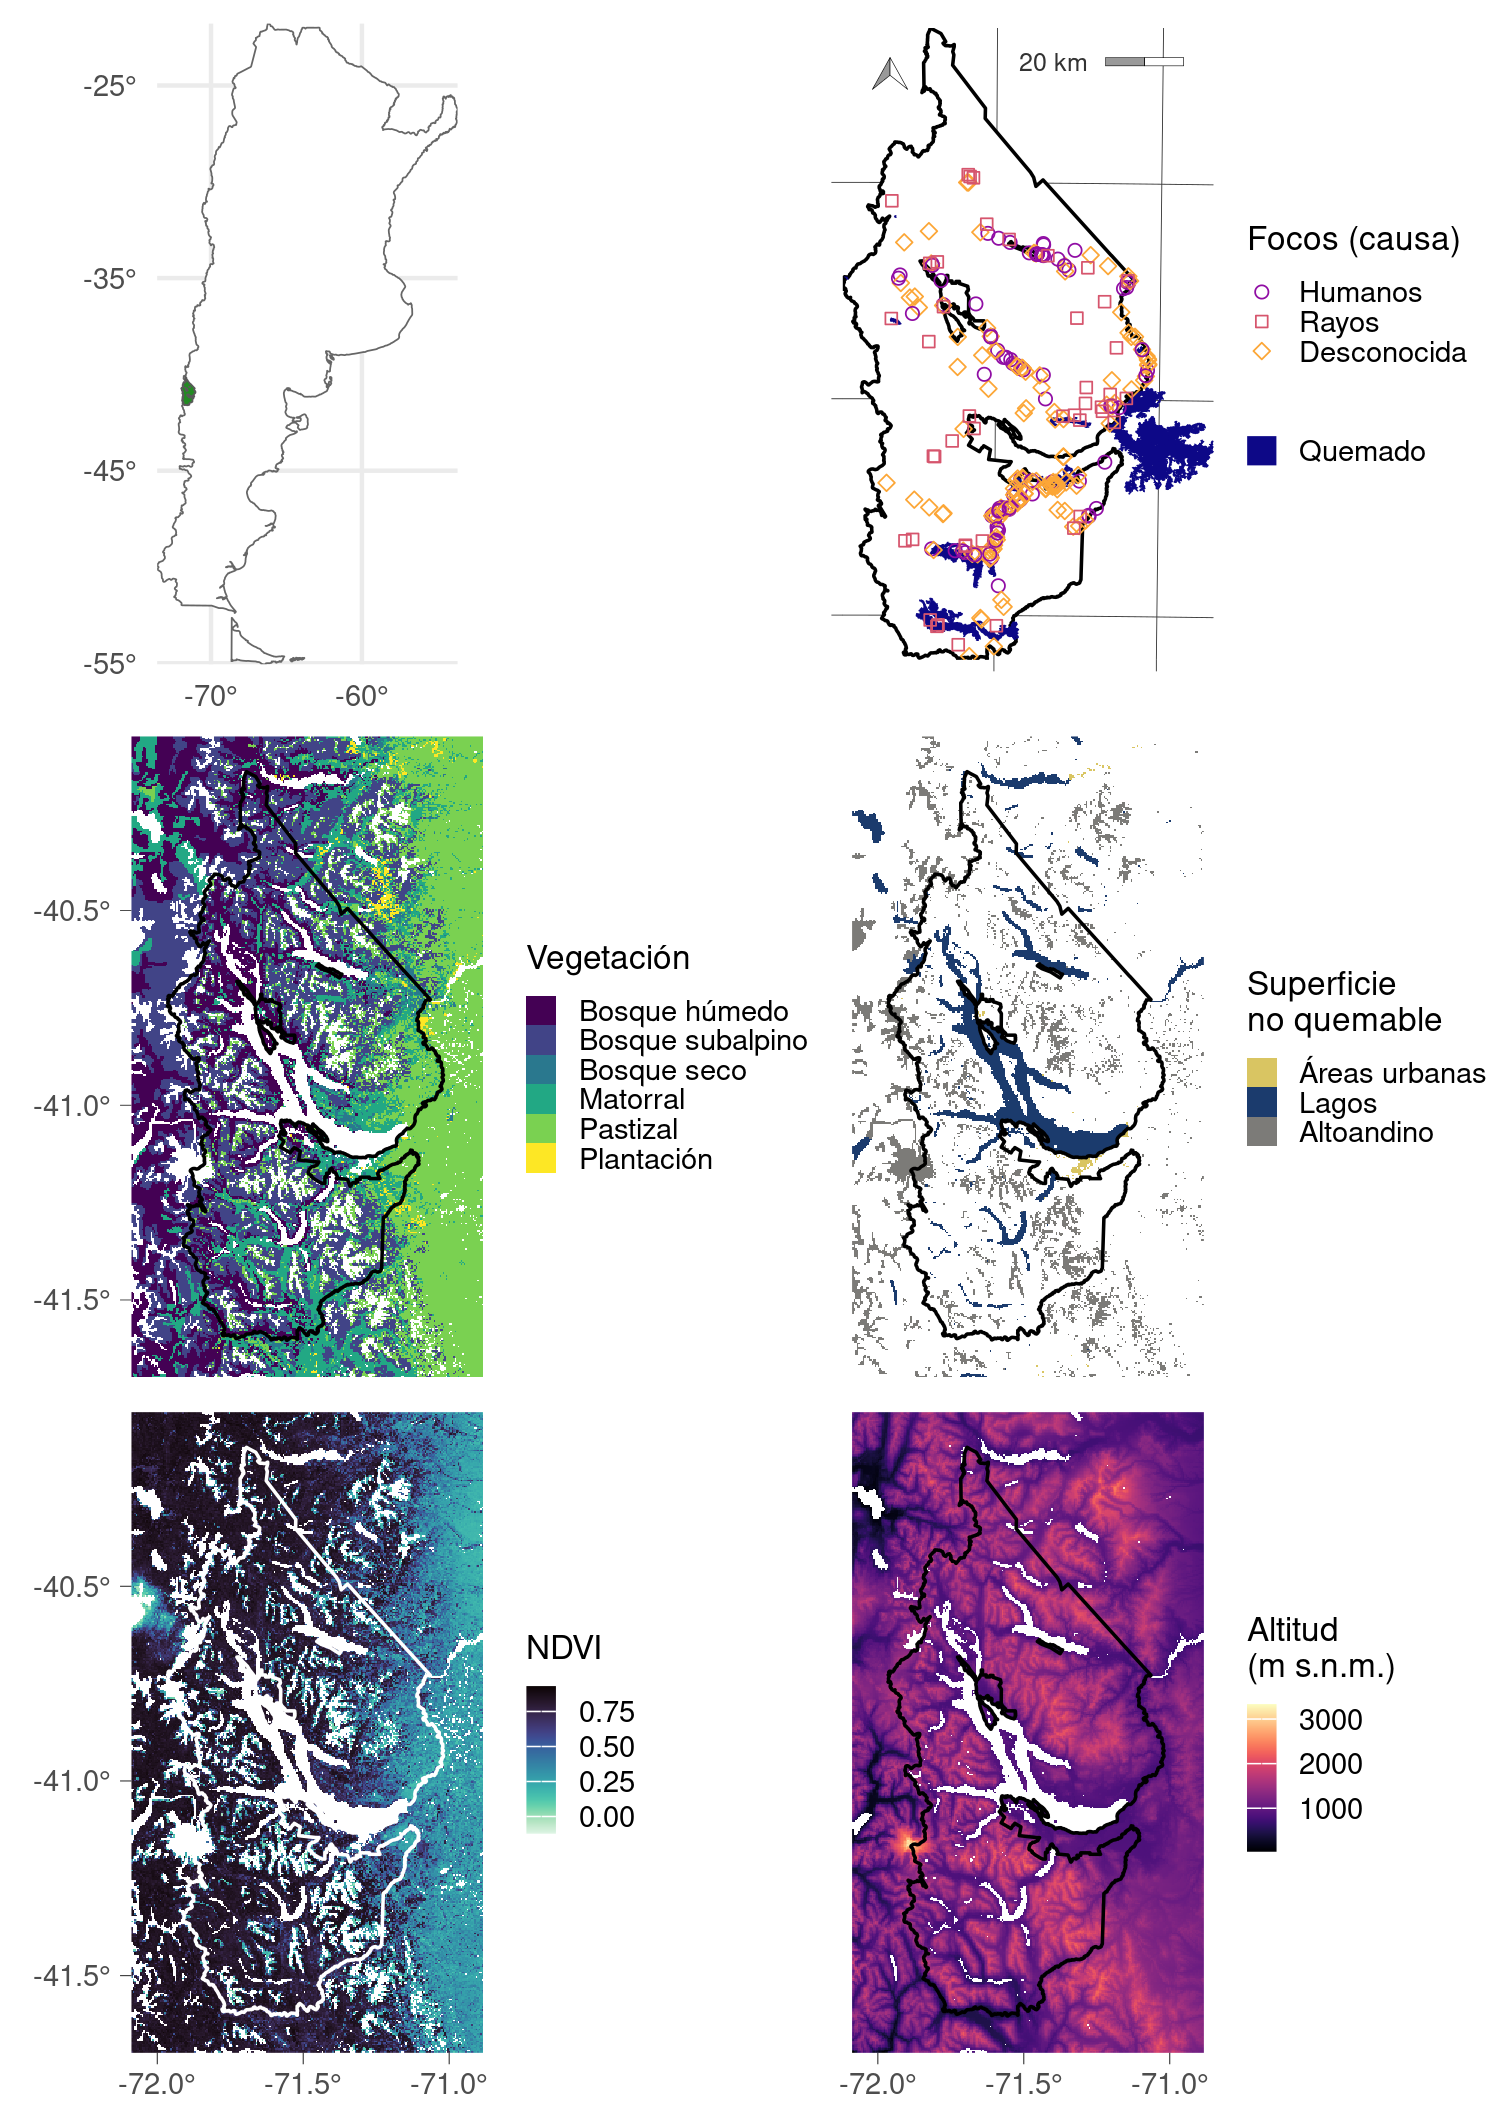
\includegraphics[width=1\textwidth]{figuras/cap4/projections/pnnh_landscape.png}
    \caption[Área de estudio, Capítulo~\ref{cap:modelos}.]{Mapas del Parque Nacional Nahuel Huapi destacando la base de datos de igniciones con el área quemada (1999-2022, mapeo del Capítulo~\ref{cap:patrones}), y algunas de las predictoras utilizadas en los modelos. Para una descripción del área de estudio, ver Sección~\ref{cap3:study-area}.} 
    \label{fig:pnnh_landscape}
\end{figure}

\subsection{Representación de los efectos de la vegetación y la topografía}

Considerar los efectos del tipo de vegetación, la productividad y la topografía sobre la inflamabilidad requería de muchos parámetros (ver Capítulo~\ref{cap:patrones}), cuya estimación presentaba un gran desafío con la información disponible. Para reducir el número de parámetros resumimos las predictoras mencionadas con dos índices: Índice de Inflamabilidad de la Vegetación (IIV), e Índice de Inflamabilidad por Topografía (IIT). En ecología es frecuente el uso de índices para resumir numerosas predictoras, y generalmente se obtienen mediante un ordenamiento de los datos según las variables a resumir (e.g., Análisis de Componentes Principales). En este caso, el enfoque fue similar, pero en vez de un ordenamiento, utilizamos los términos del predictor lineal de una regresión logística que define la probabilidad de ocurrencia de incendios a escala regional en función de las variables de interés. Este modelo fue una simplificación del modelo conjunto desarrollado en el Capítulo~\ref{cap:patrones} (ver Apéndice~\ref{append:FI}), y tomando la media de la distribución posterior de sus parámetros definimos los índices de la siguiente manera:  

\begin{equation}
\label{eq:FI}
\begin{aligned}
    IIV &= \{[\alpha_v + \beta_v \ (NDVI - \omega_v)] + 3.487888\} \ \frac{1}{1.225364} \\
    IIT &= [(-0.002407865 \ E + 0.2937129 \ N) + 2.691936] \ \frac{1}{0.852505} \\
    N & = \cos \left(L \  \frac{\pi}{180}\right) \ \frac{1}{1 + \exp(-5 + 35 \ P)},
\end{aligned}
\end{equation}

\noindent con $\alpha_v$, $\beta_v$ y $\omega_v$ definidos en la Tabla~\ref{tab:fi_params_veg} y variando por tipo de vegetación ($v$). $E$ es la altitud en m s.n.m., $N$ es el componente norte de la orientación de la ladera ($L$, en grados), y $P$ es la pendiente de la ladera (°). De esta manera, $N$ está ponderado por la pendiente, tomando valores cercanos a cero cuando la pendiente es baja. Ambos índices están escalados para tener media 0 y desvı́o 1 sobre el área de estudio del Capı́tulo~\ref{cap:patrones}. Las tablas~\ref{tab:IIV-values} y \ref{tab:IIT-values} muestran valores de estos índices para condiciones contrastantes de vegetación y topografía, y la figura~\ref{fig:FI} muestra cómo varı́an los ı́ndices en función de cada una de las variables que los definen.

\begin{table}[h]
    \centering
    \caption[Parámetros que definen el índice de inflamabilidad de la  vegetación.]{Parámetros que definen el índice de inflamabilidad de la  vegetación (IIV).}
    \label{tab:fi_params_veg}
    \begin{tabular}{l|c|c|c}
    \toprule
    Parámetro        & $\alpha$  & $\beta$    & $\omega$  \\
    \midrule
    Bosque húmedo    & -2.550628 & -44.552187 & 0.6624889 \\
    Bosque subalpino & -2.502559 & -52.508023 & 0.6988966 \\
    Bosque seco      & -2.707386 &  -3.716391 & 0.6537689 \\
    Matorral         & -2.603914 &  -4.409584 & 0.6669274 \\
    Pastizal         & -2.625388 & -10.730352 & 0.6233552 \\
    \bottomrule
    \end{tabular}
\end{table}

\begin{table}[h]
    \centering
    \caption[Índice de Inflamabilidad de la Vegetación en función del tipo de vegetación.]{Índice de Inflamabilidad de la Vegetación (IIV) en función del tipo de vegetación, para valores esperados de NDVI a 900 m s.n.m., en laderas con orientación este y con pendiente de 10°. El NDVI esperado fue predicho en base al modelo descripto en el Apéndice~\ref{append:spread-veg-effects}.}
    \label{tab:IIV-values}
    \begin{tabular}{l|rr}
    \toprule
    Tipo de vegetación & NDVI & IIV \\
    \hline
    Bosque húmedo & 0.823 & -0.176 \\
    Bosque subalpino & 0.817 & 0.209 \\
    Bosque seco & 0.664 & 0.637 \\
    Matorral & 0.703 & 0.717 \\
    Pastizal & 0.469 & 0.494 \\
    \bottomrule
    \end{tabular}
\end{table}

\begin{table}[h]
    \centering
    \caption[Índice de Inflamabilidad por Topografía para valores contrastantes de altitud y orientación.]{Índice de Inflamabilidad por Topografía (IIT) para valores contrastantes de altitud y orientación, fijando la pendiente en 10°.}
    \label{tab:IIT-values}
    \begin{tabular}{ccc}
    \toprule
    Altitud (m s.n.m.) & Orientación & IIT \\
    \hline
    500 & N & 1.808\\
    1000 & N & 0.396\\
    1500 & N & -1.016\\
    500 & E/O & 1.746\\
    1000 & E/O & 0.333\\
    1500 & E/O & -1.079\\
    500 & S & 1.683\\
    1000 & S & 0.270\\
    1500 & S & -1.142\\
    \bottomrule
    \end{tabular}
\end{table}

\FloatBarrier

\subsection{Definición y estimación de modelos}

\subsubsection{Modelo de ignición}

Definimos la ignición como la ocurrencia de un foco en una celda con vegetación con un tamaño y duración suficientes como para que el ICE del PNNH fuera notificado, excluyendo de la base de datos los focos en infraestructura humana. Separamos el proceso de ignición en dos submodelos: temporal y espacial (Fig.~\ref{fig:esquema}A). Por un lado, modelamos el número total de igniciones en toda el área de estudio (el PNNH) por quincena, separando igniciones humanas de aquellas causadas por rayos, y considerando como única predictora el FWI. Por otro lado, modelamos la ubicación de las igniciones como una regresión logística condicional, sorteando en qué celdas ocurrían las igniciones según variables espaciales de resolución media-alta (vegetación, topografía, e influencia humana; Fig.~\ref{fig:esquema}A). Si bien modelar directamente la probabilidad de ignición por celda y quincena sería más flexible, esto implicaría un alto costo computacional, ya que se requería calcular la probabilidad de ignición en todas las celdas del paisaje en cada quincena y simular un proceso de Bernoulli. Dado que el FWI tiene muy baja resolución espacial (24 km) comparado con las demás predictoras (30 m) y que la utilizamos como anomalía (i.e., sin patrón espacial en promedio), simulamos el número de igniciones en toda el área, utilizando el promedio espacial del FWI por quincena. De esta manera, sólo se debe sortear qué celdas se queman cuando las igniciones ocurren. Además, la regresión logística condicional permite aproximar el proceso simulando la ignición en un pequeño subconjunto de celdas seleccionadas al azar, en vez de calcular la probabilidad en todo el paisaje.

El modelo temporal de igniciones para el PNNH se define así:

\begin{equation}
\label{eq:igrate}
\begin{aligned}
    N_{tc} &\sim \text{Binomial Negativa}(\lambda_{tc}, \phi_{tc}) \\
    \lambda_{tc} &= \frac{\upsilon_c}{1 + \exp{(-\eta_{tc})}} \ A\\
    \eta_{tc} &= \beta_{0,c} + \beta_{1,c} \ x_t \\
    x_t &= \sum_{l=0}^{10} FWI_{t-l} \ \frac{w_l}{\sum_{j=0}^{10} w_j}\\
    w_l &= e^{-\left(\frac{l}{\tau}\right)^2}\\
    \phi_{tc} &= \gamma_{0c} + \gamma_{1c} \ \lambda_{tc} \\ 
    \\
    \upsilon_c &\sim \text{Normal}(14/A, 14/A)\text{T}[0, ] \\ 
    \beta_{0c} &\sim \text{Normal}(0, 10) \\
    \beta_{1c} &\sim \text{Normal}(0, 5)\text{T}[0, ] \\
    \gamma_{0c} &\sim \text{Normal}(0, 50)\text{T}[0, ] \\
    \gamma_{1c} &\sim \text{Normal}(0, 10)\text{T}[0, ] \\
    \tau &\sim \text{Normal}(0, 8.25)\text{T}[0, ]. 
\end{aligned}
\end{equation}
\addcontentsline{equations}{subsection}{\ref{eq:igrate} Modelo de tasa de ignición.}

\noindent $N_{tc}$ es el número de igniciones de la quincena $t$ con causa $c \in \{\text{humanos, rayos}\}$ en todo el PNNH. La distribución Binomial Negativa se parametriza con media ($\lambda$) y precisión ($\phi$), con $\text{Var}(N) = \lambda + \lambda^2 / \phi$. $\upsilon$ es el máximo que puede alcanzar la tasa de ignición por quincena y por $\text{km}^2$. En la definición de la media ($\lambda$) se incluye el factor $A$ (el área del PNNH, $7161.577\ \text{km}^2$), para escalarla al número de igniciones esperado para todo el parque. $x$ es un promedio ponderado del FWI desde la quincena focal ($t$) hasta 10 quincenas atrás ($t-10$), con los pesos decayendo de forma exponencial cuadrática hacia el pasado. La rapidez de este decaimiento es controlada por el parámetro $\tau$. La distribución Normal es parametrizada con media y desvío, con $\text{T}[0, ]$ indicando si la distribución fue truncada ([límite inferior, límite superior]), donde la omisión de un límite indica $\pm\infty$. Modelamos $\lambda$ con una función logística para evitar que las predicciones tomaran valores extremadamente altos al predecir valores fuera del rango observado de $x$. Con el mismo espíritu, definimos $\phi$ como una función lineal creciente de $\lambda$, evitando que el modelo simulara valores extremos de $N$, lo cual podía ocurrir incluso si $\lambda$ presentaba un límite superior.

El modelo espacial de igniciones ubica en el paisaje todas las igniciones simuladas por el modelo temporal en cada quincena, evaluando por separado igniciones humanas y por rayos. Este proceso se simula como un muestreo de celdas quemables sin reemplazo, en donde cada celda tiene una probabilidad inicial $\theta_i$, que depende de características del paisaje, de las cuales, sólo el índice de inflamabilidad de la vegetación (IIV) varía entre años, y ninguno varía entre quincenas. Estrictamente, la distribución de la identidad de las celdas quemadas por cada causa se podría describir como una hipergeométrica multivariada, en donde se ofrece sólo un elemento de cada ítem (celda; \citealt{fog2008calculation}). Sin embargo, dado que el número de celdas quemadas es notablemente menor al número de celdas quemables, la verosimilitud se puede aproximar usando la distribución categórica, tratando por separado cada ignición, lo que equivale a suponer $N_{tc} = 1$ bajo la formulación hipergeométrica:

\begin{equation}
\label{eq:igspat}
\begin{aligned}
    i_{tc} &\sim \text{Categórica}(\boldsymbol{\theta}_{tc}) \\
    \theta_{itc} &= \frac{\exp{(\eta_{itc})}}{\sum_{j=0}^{C_t} \exp{(\eta_{jtc})}} \\
    \eta_{itc} &= \beta_{1c} \ IIV_{it} + \beta_{2c} \ IIT_i + \beta_{3c} \ DP_i + \beta_{4c} \ DC_i\\
    \\
    \beta_{kc} &\sim \text{Normal}(0, 10)T[0, ] \  \text{para} \ k \in \{1, 2\} \\
    \beta_{kc} &\sim \text{Normal}(0, 10)T[, 0] \  \text{para} \ k \in \{3, 4\} \ \text{y}\  c = \text{humanos} \\
    \beta_{kc} &= 0 \  \text{para} \ k \in \{3, 4\} \ \text{y}\  c = \text{rayos}.
\end{aligned}
\end{equation}

\noindent $i_{tc} \in \{1, ..., C_t\}$ identifica cada celda quemable del PNNH en la quincena $t$, mientras que $C_t$ es el número total de celdas quemables. $\boldsymbol{\theta}$ es un vector de probabilidades de largo $C_t$ que suma 1, y se calcula a partir de los predictores lineales, $\eta_i$. $IIV$ e $IIT$ son los índices de inflamabilidad de la vegetación y por topografía, respectivamente, definidos en \eqref{eq:FI}; $DP$ y $DC$ representan la distancia al poblado y al camino más cercano, respectivamente. Nótese que los coeficientes que multiplican dichas distancias están restringidos a ser negativos en el caso de igniciones humanas (mayor distancia, menor probabilidad relativa de ignición), y son fijados en cero para las igniciones por rayos. A su vez, los coeficientes de los índices de inflamabilidad están restringidos a ser positivos (mayor inflamabilidad, mayor probabilidad relativa de ignición). Cabe remarcar que para estimar estos modelos sólo contábamos con datos de focos, sin poder separar el proceso de ocurrencia de rayos u ocurrencia de una fuente de calor generada por humanos (e.g., una brasa que vuela desde una fogata) de la subsiguiente propagación a pequeña escala que genera un foco detectable. Por este motivo, consideramos que la vegetación y la topografía pueden afectar la ocurrencia de focos, tanto naturales como antrópicos, no por determinar dónde se producen rayos o fuentes de calor antrópicas, sino por regular la propagación inicial que define si la fuente de calor se llega a convertir en un foco. 

Incluso utilizando la aproximación categórica, calcular los $\theta_{itc}$ para todas las celdas del paisaje es altamente costoso, tanto para realizar simulaciones como para ajustar el modelo. Por lo tanto, utilizamos una segunda aproximación. Para estimar el modelo representamos el conjunto de celdas quemables del paisaje con una muestra al azar de 10000 celdas. Como la única predictora que varía en el tiempo es el IIV, este se calcula para todos los años en que tenemos datos (focos) para esas 10000 celdas. De esta manera, al ajustar el modelo calculamos únicamente 10000 $\times$ años valores de $\eta_i$ para cada causa (los coeficientes varían entre causa humana o por rayos). Así, los $\theta_{itc}$ asociados a cada ignición observada se calculan sobre una muestra compuesta por la celda en donde se observó la ignición y las 10000 celdas potenciales. Para simular el proceso, tomamos una muestra de 2000 celdas para cada causa, a modo de reducir aún más el costo computacional, ya que las simulaciones requieren repetir esto en cada quincena. 

El modelo fue estimado con enfoque bayesiano, usando Stan para muestrear la distribución posterior de los parámetros \citep{stan_development_team_rstan_2022}. Corrimos 8 cadenas markovianas de Monte Carlo, por 2500 iteraciones cada una, dejando 1500 para \textit{warm-up}. El muestreo convergió ($\hat{R}_{\text{max}} = 1.002096$) y se obtuvo un número efectivo de muestras suficiente (mínimo = $2478.018$).

\subsubsection{Modelo de escape}

Dado que una gran proporción de focos no llega a extenderse por más de una celda de 30 m, definimos como escape al hecho de que un foco propagara fuera de la celda en que se originó \citep{marchal_turning_2020}. El modelo de escape es una regresión logística que determina la probabilidad de que el fuego escape de la celda en que se inició (Fig.~\ref{fig:esquema}B). Entre las predictoras se incluyen la vegetación, la topografía, la influencia humana y el tiempo atmosférico, y los parámetros no varían entre igniciones causadas por humanos o por rayos:

\begin{equation}
\label{eq:escape}
\begin{aligned}
    y_{it} &\sim \text{Bernoulli}(\theta_{it}) \\
    \theta_{itc} &= \frac{1}{1 + \exp{(-\eta_{it})}} \\
    \eta_{it} &= \beta_0 + \beta_1 \ IIV_{it} + \beta_2 \ IIT_i + \beta_3 \ DP_i + \beta_4 \ DC_i + \beta_5 \ x_{it} \\
    x_{it} &= \sum_{l=0}^{10} FWI_{i,t-l} \ \frac{w_l}{\sum_{j=0}^{10} w_j} \\
    w_l &= e^{-\left(\frac{l}{\tau}\right)^2}\\
    \
    \\
    \beta_0 &\sim \text{Normal}(0, 3) \\ 
    \beta_k &\sim \text{Normal}(0, 5)\text{T}[0, ] \  \text{para} \ k \in \{1, 2, 5\} \\
    \beta_k &\sim \text{Normal}(0, 5) \  \text{para} \ k \in \{3, 4\} \\
    \tau &\sim \text{Normal}(0, 8.25)\text{T}[0, ]. 
\end{aligned}
\end{equation}

\noindent $y_{it} \in \{0, 1\}$ indica si la ignición ocurrida en la celda $i$ en la quincena $t$ propagó fuego a sus vecinas. Nuevamente, el IIV varía entre años, por lo que en todas las quincenas del mismo año toma el mismo valor. El efecto de dicha variable, así como los efectos del IIT y del FWI fueron restringidos a tomar valores positivos. 

El modelo fue estimado con enfoque bayesiano, usando Stan \citep{stan_development_team_rstan_2022}. Corrimos 8 cadenas markovianas de Monte Carlo, por 2500 iteraciones cada una, dejando 1500 para \textit{warm-up}. El muestreo convergió ($\hat{R}_{\text{max}} = 1.0032$) y se obtuvo un número efectivo de muestras suficiente (mínimo = $1998.468$).

\subsubsection{Modelo de propagación}\label{cap4:spread-model}

El modelo de propagación simula el contagio del fuego desde celdas encendidas a sus 8 vecinas, con una estructura muy similar al propuesto por Morales et al. (\citealt{morales_stochastic_2015}; Fig.~\ref{fig:esquema}C). Si bien la simulación es un proceso iterativo, se asume que los incendios transcurren enteramente en una quincena, es decir, el modelo es atemporal dentro de ese período. Las celdas tienen tres estados posibles: encendida, quemable, y no quemable. Las celdas encendidas sólo pueden mantenerse así durante una iteración (paso de ahora en más), luego de la cual se vuelven no quemables (quemadas). Algunas celdas pueden ser no quemables desde el comienzo, como aquellas ubicadas sobre cuerpos de agua o zonas no vegetadas, o quemadas en una quincena previa en el mismo año. La simulación comienza con al menos una celda quemada, y en cada paso, se simula la propagación desde cada celda encendida a sus vecinas quemables como un proceso Bernoulli. El paso se completa una vez que se simuló propagación desde todas las celdas encendidas. La probabilidad de propagación se define como una función logística de las variables ambientales. Los términos de esta función corresponden al IIV e IIT de la celda receptora y a efectos direccionales del viento y la pendiente, los cuales se calculan a partir de variables correspondientes a las celdas dadora y receptora. Se asume que la distancia a caminos y poblados no afectan la probabilidad de propagación. Las celdas receptoras con más de una vecina encendida pueden recibir fuego de todas ellas; es decir, si la primera vecina no la quema, puede ser quemada por la segunda, y así sucesivamente hasta completar la revisión de sus vecinas encendidas (máximo 8). En ese proceso, el orden en que se simula la propagación desde sus vecinas es indistinto. La simulación termina cuando se alcanza el máximo número de pasos, pero puede terminar antes si, por azar, ninguna celda encendida logra propagar fuego a sus vecinas. 
La propagación $y \in \{0, 1\}$ desde la celda $i$ hacia una celda vecina quemable $j$ en el paso $k$ se define de la siguiente manera:

\begin{equation}
\label{eq:datamodel}
\begin{aligned}
    y_{ijk} &\sim \ \text{Bernoulli}(\theta_{ijk}) \\
    \theta_{ijk} &= \frac{\mathbb{I}_{k \le \kappa}}{1 + \exp{(-\eta_{ij})}} \\
    \eta_{it} &= \beta_0 + \beta_1 \ IIV_j + \beta_2 \ IIT_j + \beta_3 \ S_{ij} + \beta_4 \ W_{ij} \\
    S_{ij} &= \sin\left[ \tan^{-1} \left( \frac{E_j - E_i}{G_{ij}} \right) \right] \, \mathbb{I}_{E_j - E_i > 0}, \\
    W_{ij} &= \cos(A_{ij} - D_i) \ V_i
\end{aligned}
\end{equation}

\noindent $\theta$ es la probabilidad de propagación, y $\mathbb{I}_{k \le \kappa}$ es una variable indicadora que toma 1 si el número de pasos, $\kappa$, no ha sido superado, y 0 en caso contrario. $S_{ij}$ y $W_{ij}$ son términos que representan los efectos direccionales de la pendiente y el viento, respectivamente. $E$ es la altitud sobre el nivel del mar de cada celda (m), $G_{ij}$ es la distancia (m) entre celdas, $A_{ij}$ es la dirección desde donde llegaría el fuego, es decir, la posición de la celda dadora vista desde la receptora (radianes), $D_i$ es la dirección desde donde sopla el viento en la celda dadora (radianes), y $V_i$ es la velocidad del viento en la celda dadora (m/s). El primer factor en $S_{ij}$ es el seno de la pendiente entre las celdas, de tal forma que toma 1 si la celda receptora se encuentra exactamente arriba de la dadora, -1 si está exactamente debajo, y 0 si están a la misma altitud. Pero como las celdas no se solapan, su valor no suele superar $0.7101 = \sin{(45\ \text{°})}$. La variable indicadora $\mathbb{I}_{E_j - E_i > 0}$ anula este término en caso de que la propagación ocurra cuesta abajo. El primer factor en $W_{ij}$ toma 1 cuando el viento sopla en la misma dirección y sentido que la propagación, -1 si sopla en la misma dirección pero sentido opuesto, y 0 si sopla perpendicular a la dirección de las celdas dadora y receptora. La velocidad $V_i$ le da magnitud a este término. Dado que el vecindario está conformado por las 8 celdas vecinas de la celda dadora, las distancias entre celdas $G_{ij}$ y las direcciones $A_{ij}$ (en ángulos) pueden representarse mediante los siguientes esquemas:

\[
    G =
    \begin{bmatrix}
        30 \ \sqrt{2} & 30 & 30 \ \sqrt{2} \\
        30 & \cdot & 30 \\
        30 \ \sqrt{2} & 30 & 30 \ \sqrt{2}
    \end{bmatrix}, \quad
    A =
    \begin{bmatrix}
        135 & 180 & 225 \\
        90 & \cdot & 270 \\
        45 & 0 & 315
    \end{bmatrix},
\]

\noindent donde $\cdot$ representa la posición de la celda dadora, y 30 m es el tamaño de las celdas. Finalmente, los parámetros $\beta$ y $\kappa$ son cantidades desconocidas, y deben ser estimados. De ahora en más, los denominaremos conjuntamente como el vector $\boldsymbol{\beta}$:

\begin{equation}\label{eq:spread_params}
    \boldsymbol{\beta} = \{\beta_1, \beta_2, \beta_3, \beta_4, \beta_5, \kappa\}.
\end{equation}

Uno de nuestros principales objetivos era modelar los efectos de las condiciones atmosféricas sobre la propagación. Sin embargo, en la región hay una densidad muy baja de estaciones meteorológicas como para obtener datos con adecuada resolución espacial y temporal en grandes extensiones y para muchos años. Por lo tanto, obtuvimos el FWI de \citet{vitolo_era5-based_2020}, que se basa en el reanálisis climático del ERA5 \citep{hersbach2020era5}, con resolución temporal diaria y espacial de aproximadamente 24 km (0.25°). A partir de los datos diarios estandarizados a nivel de píxel, calculamos los promedios por quincena, y luego utilizamos su valor acumulado, como un promedio ponderado de la quincena focal y las anteriores, tal como en los modelos de ignición y escape. Con una resolución espacial gruesa para el FWI y con una baja variabilidad espacial (debido a la estandarización), optamos por asumir que el clima es constante en cada incendio, tomando su valor interpolado en la celda de ignición. De esta manera, incluimos el efecto de la meteorología en el modelo, modelando los parámetros de propagación ($\boldsymbol{\beta}$) como una función del FWI estandarizado, promediado y acumulado por quincena. Pero aún incluyendo esta variación, el modelo seguía siendo una representación demasiado simple de la propagación del fuego, en gran parte porque, a falta de datos, se asume que la dirección y velocidad regional del viento son constantes durante toda la simulación y no se consideran los efectos del combate del fuego en la propagación. Por lo tanto, para representar mejor la variabilidad de proceso no contemplada en el modelo especificamos un modelo estadístico para los parámetros, es decir, le dimos estructura jerárquica (i.e., modelo mixto o multinivel). Esto significa que el FWI no define de forma determinística los parámetros de propagación, sino que define la media de una distribución de parámetros. De esta manera, incendios con el mismo valor de FWI pueden presentar distintos parámetros. Esta estrategia de modelado permite representar variabilidad entre incendios en muchas variables no contempladas por el modelo (meteorología, combate del fuego, particularidades del terreno como humedad del suelo, etc.). El modelo de parámetros (para $\boldsymbol{\beta}$) fue definido de la siguiente manera:

\begin{equation}
\label{eq:hier1}
\begin{aligned}
    \boldsymbol{\beta}_{ft} &= \textbf{L} + \frac{\textbf{U} - \textbf{L}}{1 + \exp{(\boldsymbol{\eta}_{ft}})} \\
    \boldsymbol{\eta}_{ft} &\sim \ \text{Normal Multivariada}(\boldsymbol{\mu}_{ft}, \boldsymbol{\Sigma}) \\
    \boldsymbol{\mu}_{ft} &= \boldsymbol{\gamma}_0 + \boldsymbol{\gamma}_1 \ x_{ft} \\
    x_{ft} &= \sum_{l=0}^{10} FWI_{f,t-l} \ \frac{w_l}{\sum_{j=0}^{10} w_j} \\
    w_l &= e^{-\left(\frac{l}{\tau}\right)^2},
\end{aligned}
\end{equation}

\noindent donde $\boldsymbol{\beta}_{ft}$ es el vector de parámetros asociado al fuego $f$, ocurrido en la quincena $t$. $\textbf{L}$ y $\textbf{U}$ son los vectores con los límites inferiores y superiores, respectivamente, para cada parámetro que conforma el vector $\boldsymbol{\beta}_{ft}$. Restringir los parámetros permitió simplificar el proceso de estimación y facilitó aplicar restricciones de signo. De esta manera, los $\boldsymbol{\beta}_{ft}$ siguen una distribución Logit-Normal Multivariada, escalada entre $\textbf{L}$ y $\textbf{U}$. La Normal Multivariada está parametrizada por su vector de medias $\boldsymbol{\mu}$ y la matriz de varianza-covarianza $\boldsymbol{\Sigma}$. Para simplificar la estimación, el parámetro $\tau$ fue obtenido de un modelo de tamaño de incendios en función del FWI acumulado ($x$), y fijado en el modo de la posterior conjunta: $2.82$. Los límites de los parámetros fueron definidos de la siguiente manera:

\begin{equation}
\label{eq:limits}
\begin{aligned}
    \textbf{L} &= \{-50, 0, 0, 0, 0, 2\} \\
    \textbf{U} &= \{-50, 30, 30, 158.6232, 30, \psi\} \\ 
    \psi &\sim \ \text{Uniforme}(1150, 2000), \\
\end{aligned}
\end{equation}

\noindent estimando el límite superior de los pasos de simulación ($\text{U}_6 = \psi$). El límite superior en la previa de $\psi$ se fijó en 2000 porque eso implica que el fuego puede recorrer como máximo 60 km ($2000 \ \text{pasos} \times 30 \ \text{m} = 60000 \ \text{m}$), lo cual abarca la extensión oeste-este de los bosques andino-patagónicos en Argentina. Si bien podrían ocurrir incendios más grandes, se escaparían de nuestra área de estudio, y carecemos de datos para informar la probabilidad de propagación en la estepa. El límite inferior de $\psi$ se definió como el máximo valor que presentaba buen ajuste para los incendios utilizados en la estimación. 

La predictora $x$ fue estandarizada previo a la estimación, y utilicé las siguientes previas para los coeficientes de la regresión de la media ($\boldsymbol{\mu}$, en escala logit):

\begin{equation}
\begin{aligned}
    \gamma_{0p} &\sim 
    \begin{cases} 
        \text{Normal}(0, 10), & \text{para } p \in \{1, \ldots, 5\}, \\
        \text{Normal}(-3.80, 10), & \text{para } p = 6.
    \end{cases} \\
    \boldsymbol{\gamma_{1}} &\sim \ \text{Normal}(0, 10),
\end{aligned}
\end{equation}

\noindent donde el subíndice $p \in \{1, ..., 6\}$ identifica los hiperparámetros asociados a cada parámetros de propagación ($\boldsymbol{\beta}$).
 
La matriz $\boldsymbol{\Sigma}$ fue descompuesta en un vector de desvíos estándar ($\boldsymbol{\sigma}$) y una matriz de correlación ($\boldsymbol{\Omega}$) para asignarle una previa más flexible: 

\begin{equation}
\label{eq:hier2}
\begin{aligned}
    \boldsymbol{\Sigma} &= \text{diag}(\boldsymbol{\sigma}) \ \boldsymbol{\Omega} \ \text{diag}(\boldsymbol{\sigma}) \\
    \sigma_p^2 &\sim \ \text{Gama Inversa}(\alpha = 1, \beta = 0.001) \\
    \boldsymbol{\Omega} &= \text{diag}(\boldsymbol{V})^{-\frac{1}{2}} \, \boldsymbol{V} \, \text{diag}(\boldsymbol{V})^{-\frac{1}{2}}  \\
    \boldsymbol{V} &\sim \ \text{Wishart Inversa}(\nu = 7, \boldsymbol{\Sigma} = \boldsymbol{I}).    
\end{aligned}
\end{equation}

\noindent La matriz de varianza-covarianza $\boldsymbol{V}$ es una variable accesoria, utilizada únicamente para asignarle una previa Wishart Inversa a la matriz de correlación, sin que los parámetros de dicha previa afecten a los desvíos estándar ($\boldsymbol{\sigma}$). Los parámetros de la Wishart-Inversa generan una distribución aproximadamente uniforme entre -1 y 1 para los coeficientes de correlación. La densidad de la distribución Gama Inversa se define como $f(x) = \alpha^\beta/\Gamma(\beta) x^{(-1-\beta)} e^{(-\alpha/x)}$. $\boldsymbol{I}$ representa la matriz identidad.

Dado que modelamos una distribución de probabilidad (la Normal Multivariada) para los parámetros de propagación ($\boldsymbol{\beta}$), los incendios ya ocurridos y con punto de ignición conocido pueden ser simulados utilizando nuevos parámetros $\boldsymbol{\beta}$ simulados a partir de dicha distribución, en base al FWI asociado a dicho incendio, o pueden ser simulados utilizando el vector $\boldsymbol{\beta}$ estimado específicamente para ese incendio. A estos dos casos les llamamos, respectivamente, \textit{parámetros simulados} y \textit{parámetros ajustados} (ver Fig.~\ref{fig:spread-ov} y \ref{fig:spread-q}). 

Para estimar la mayor parte de los parámetros de propagación utilizamos 57 incendios con punto de ignición conocido, simulando incendios con el modelo bajo las mismas condiciones (ver detalles abajo). Sin embargo, estos incendios representaban un subconjunto de mayor tamaño en relación a los 235 incendios $\ge10$ ha mapeados (\cref{cap:patrones}), lo cual habría sesgado la estimación de los parámetros que controlan el tamaño del incendio simulado, a saber, el número de pasos ($\kappa_f$, Ecuación~\ref{eq:datamodel}) y sus hiperparámetros ($\gamma_{0,6}$, $\gamma_{1, 6}$, y $\sigma_6$; ver Ecuación~\ref{eq:hier1}). Para corregir este sesgo estimamos un modelo accesorio, que relacionando los pasos estimados de 57 incendios con su tamaño permitía inferir los pasos requeridos para los 178 incendios con punto de ignición desconocido que no se podían simular: 

\begin{equation}
\begin{aligned}
    \log(a_f) &\sim \ \text{Normal}(\mu_f, \sigma_a)\text{T}[\log(10), ] \\
    \mu_f &= \alpha_0 + \alpha_1 \ \log(\kappa_f) \\
    \alpha_0 &\sim \ \text{Normal}(-1.52, 10) \\
    \alpha_1 &\sim \ \text{Normal}(0, 10), \\
\end{aligned}
\end{equation}

\noindent donde $a_f$ es el área del incendio $f$ (ha). La previa sobre $\alpha_0$ fue centrada en la media de $\log(a)$ sobre los 235 incendios para no sesgar su estimación.

Estimar el modelo de propagación presentó un desafío considerable porque no contaba con datos de propagación celda a celda ($y_{ijk}$ en Ecuación~\ref{eq:datamodel}). Es decir, en el mejor caso, se conoce el punto de ignición y el polígono final de un incendio, pero no se sabe cómo el fuego propagó celda a celda (y tampoco sería posible registrarlo, ya que el fuego avanza de forma continua en el tiempo y en el espacio). Sin datos sobre el contagio celda a celda, no podíamos evaluar la función de verosimilitud, por lo que utilizamos Computación Bayesiana Aproximada (ABC, por sus siglas en inglés; \citealt{sisson2018handbook,beaumont2010approximate}), también usado para este fin por \citet{morales_stochastic_2015}. Este enfoque se aplica en casos donde tenemos un modelo capaz de simular datos pero no podemos evaluar de forma directa la función de verosimilitud. Básicamente consta en seleccionar los valores de los parámetros que simulen datos similares a los observados. En este caso, eso implica escoger valores de parámetros que simulen incendios similares a los observados, siempre utilizando los datos bajo los cuales sucedió cada incendio (variables espaciales, condiciones atmosféricas y punto de ignición). En el enfoque bayesiano tradicional, la distribución posterior de los parámetros ($\theta$), condicionada en los datos ($y$) se define como $p(\theta | y_{\text{obs}}) = p(y_{\text{obs}} | \theta) \ p(\theta) \ C$, donde $p(\theta | y_{\text{obs}})$ es la densidad posterior de los parámetros, $p(y_{\text{obs}} | \theta)$ es la verosimilitud, $p(\theta)$ es la densidad previa de los parámetros, y $C$ es una constante normalizadora que generalmente puede ignorarse al momento de la estimación. En ABC, la posterior no condiciona en los datos directamente sino en una medida de resumen de los mismos ($s_{\text{obs}}$):

$$p_{ABC}(\theta | s_{\text{obs}}) \propto \int K(||s_{\text{obs}} - s||) \ p(s | \theta) \ p(\theta) \ ds,$$

\noindent donde $s_{\text{obs}}$ es una medida de resumen de los datos observados, y $s$, de datos simulados por el modelo. $K()$ es una función que mapea de distancias a densidades o probabilidades, usualmente aumentando a menor distancia (\textit{kernel}), y $||\cdot||$ es alguna medida de distancia o disimilitud. $p(s | \theta)$ es una función de verosimilitud para la medida de resumen $s$ que no se puede evaluar, derivada de $p(y | \theta)$ y de $s = S(y)$. En casi todas las aplicaciones, la integración sobre $s$ se logra mediante simulación. 

En nuestro caso, $y_{\text{obs}}$ sería un vector binario (no observado), para cada incendio, indicando si el fuego propagó o no desde cada celda quemada a sus vecinas quemables, y $s_{\text{obs}} = S(y_{\text{obs}})$ es el conjunto de celdas quemadas por el incendio. Nuestra métrica de disimilitud es $||s_i - s_j|| = 1 - O_{ij}$, donde $O_{ij}$ es el solapamiento espacial entre el incendio observado y un incendio simulado: 

\begin{equation}
\label{eq:overlap}
O_{ij} = \frac{|A_i \cap A_j|}{|A_i \cup A_j|}.
\end{equation}

\noindent $O_{ij} \in [0, 1]$ toma 1 si los incendios son exactamente iguales y 0 si no comparten ni una celda quemada. $A$ indica el conjunto de celdas quemadas por cada incendio, de forma que el numerador es el número de celdas quemadas por ambos incendios, y el denominador, el número de celdas quemadas por al menos uno de los dos. Para obtener una densidad no normalizada a partir de esta métrica definimos un \textit{kernel} exponencial cuadrático:

\[
\begin{aligned}
    K[O_f(\boldsymbol{\beta})] &= \exp\{-[d_f(\boldsymbol{\beta}) / 0.025]^2\} \\
    d_f(\boldsymbol{\beta}) &= 1 - \text{min}\left[1, \frac{O_f(\boldsymbol{\beta})} {T_f}\right],
\end{aligned}
\]

\noindent donde $d_f(\boldsymbol{\beta})$ es una medida de disimilitud entre el incendio observado $f$ y un incendio simulado bajo el vector de parámetros $\boldsymbol{\beta}$, que controla la probabilidad de propagación según~\eqref{eq:datamodel}. $O_f(\boldsymbol{\beta})$ es su correspondiente valor de solapamiento espacial (Ecuación~\ref{eq:overlap}), y $T_f$ es un valor de solapamiento alto para el incendio $f$. Nótese que aquí las variables varían entre incendios porque definimos un modelo jerárquico, estimando un vector de parámetros $\boldsymbol{\beta}$ para cada incendio observado (Ecuación~\ref{eq:hier1}). Para definir $T_f$ exploramos el espacio de parámetros para cada incendio con un esquema estocástico que aseguraba encontrar regiones de alto solapamiento, simulando 50000 incendios con distintas combinaciones de parámetros. Posteriormente, $T_f$ fue definido como el mínimo solapamiento de los mejores 500 valores obtenidos (percentil 99 \%). Tanto para esta exploración como para muestrear la distribución posterior, los parámetros fueron restringidos entre $\boldsymbol{L}$ y $\boldsymbol{U}$ definidos en Ecuación~\ref{eq:limits}. Sin embargo, para reducir el costo computacional, variamos el máximo número de pasos de simulación ($U_6$, el límite para $\kappa$ en Ecuación~\ref{eq:datamodel}) entre incendios, de forma tal que su valor más alto permitiera simular fuegos tanto más grandes que el observado como para obtener un solapamiento de $\approx 0.05$, lo cual es un valor muy bajo que fácilmente se mejora utilizando menos pasos.

Debido al gran número de parámetros que presentaba el modelo, a la naturaleza estocástica de $K()$ y probablemente a sus abruptas variaciones en función de $\boldsymbol{\beta}$, las técnicas convencionales de muestreo, como cadenas markovianas de Monte Carlo (MCMC por sus siglas en inglés), presentaban un costo computacional prohibitivo. Resolvimos esto combinando dos estrategias poco comunes: por un lado, utilizamos el método de \citet{lunn2013fully}, que consiste en estimar modelos jerárquicos en (al menos) dos pasos. En el primer paso se estima la distribución posterior de los parámetros a nivel de datos ($\boldsymbol{\beta}_f$ en nuestro caso, Ecuación~\ref{eq:datamodel}) de forma separada para cada grupo (incendio, $f$), y luego se combinan las muestras de dichas distribuciones para estimar los hiperparámetros ($\boldsymbol{\gamma}_0$, $\boldsymbol{\gamma}_1$, $\psi$, $\boldsymbol{\sigma}$, y $\boldsymbol{\Omega}$; ver Ecuaciones~\ref{eq:hier1},~\ref{eq:limits}, y~\ref{eq:hier2}). Al separar el modelo en dos partes, pudimos tratar el paso dificultoso de estimar los $\boldsymbol{\beta}_f$ con mayor flexibilidad. El método de Lunn requiere que en el primer paso se defina una distribución previa sustituta para cada $\boldsymbol{\beta}_f$, cuya influencia es descontada en el segundo paso, al estimarse los hiperparámetros que constituyen la verdadera previa de los primeros. La segunda estrategia fue explotar la sustitución de la previa para generar una que aumentara la eficiencia de un muestreo por rechazo. Utilizamos lo que llamamos \textit{previas redundantes} para los $\boldsymbol{\beta}_f$ y distribuciones de propuestas con forma similar a $K(\boldsymbol{\beta_f})$. Estas estrategias lograron una eficiencia aceptable del muestreo por rechazo. Para definir las previas redundantes y la distribución de propuestas utilizamos las 50000 simulaciones del período de exploración del espacio de parámetros. Para cada simulación calculamos $K()$ y remuestreamos 10000 vectores de parámetros con reemplazo, con probabilidad proporcional a $K()$. Como distribución previa redundante utilizamos una Normal Multivariada ajustada a esas muestras incrementando los desvíos estándar por un factor de 5. Como distribución de propuesta utilizamos una distribución Normal Multivariada Asimétrica ajustada a las muestras. Para que estas distribuciones fueran medianamente razonables, trabajamos en el espacio de parámetros no restringido ($\boldsymbol{\eta}$, ver~\ref{eq:hier1}). En este paso utilizamos un muestreo por rechazo adaptado a simuladores costosos (ver sección 4.2.3.4 en \citep{sisson2018handbook}) hasta obtener un número efectivo de muestras $\ge 10000$. En el paso 2, corrimos un MCMC sobre todos los parámetros, pero utilizando las muestras del paso 1 como distribución de propuestas para los $\boldsymbol{\beta}_f$, descontando el efecto de las previas sustitutas (redundantes) del paso 1, y utilizando actualizaciones Gibbs para la mayor parte de los hiperparámetros \citep{lunn2013fully}.

Escribimos el simulador de incendios en \cpp con la colaboración de Iván Renison, quien lo estructuró en el paquete de R \texttt{FireSpread} (\url{http://github.com/barberaivan/FireSpread.git}), a través de \texttt{Rcpp} \citep{Rcpp}. Tanto para el modelo de propagación como para los anteriores utilizamos R 4.2.0 \citep{R}. El código se encuentra disponible en GitHub (\url{https://github.com/barberaivan/fire_spread}). Para manejar datos espaciales utilizamos el paquete \texttt{terra} \citep{terra}.

\subsubsection{Simulador del régimen de incendios}



Este modelo integra los procesos de ignición, escape y propagación, simulándolos en todas las quincenas de un año (Fig.~\ref{fig:esquema}). La capa de vegetación se fija utilizando el NDVI promedio del verano anterior para calcular el IIV. Las celdas quemadas en cada quincena no pueden ser quemadas nuevamente en las sucesivas quincenas. Para calibrar este modelo al PNNH, disminuimos el intercepto de la regresión de pasos ($\gamma_{0,6}^* = \gamma_{0,6} - 0.95$) para que la probabilidad de quema anual se asemejara a la registrada en el parque de acuerdo a los datos del Capítulo~\ref{cap:patrones} (período 1999-2022). Esta corrección fue necesaria porque el modelo de propagación fue ajustado a incendios $\ge 10$ ha, no a la distribución completa del tamaño de incendios, ya que no contábamos con suficientes datos para tal fin. 

Este modelo toma como entrada un ráster de FWI quincenal para todo un año en el PNNH, y devuelve un ráster binario indicando qué celdas se quemaron, a 30 m de resolución. Simulando este proceso por muchas iteraciones se puede obtener un mapa de probabilidad de quema anual calculando en qué fracción de los años simulados (iteraciones) se quemó cada celda del paisaje. A su vez, también se pueden calcular la proporción del área quemable del PNNH que se quema cada año y la proporción del área quemada correspondiente a igniciones por rayos.

\begin{figure}[H]
    \centering
    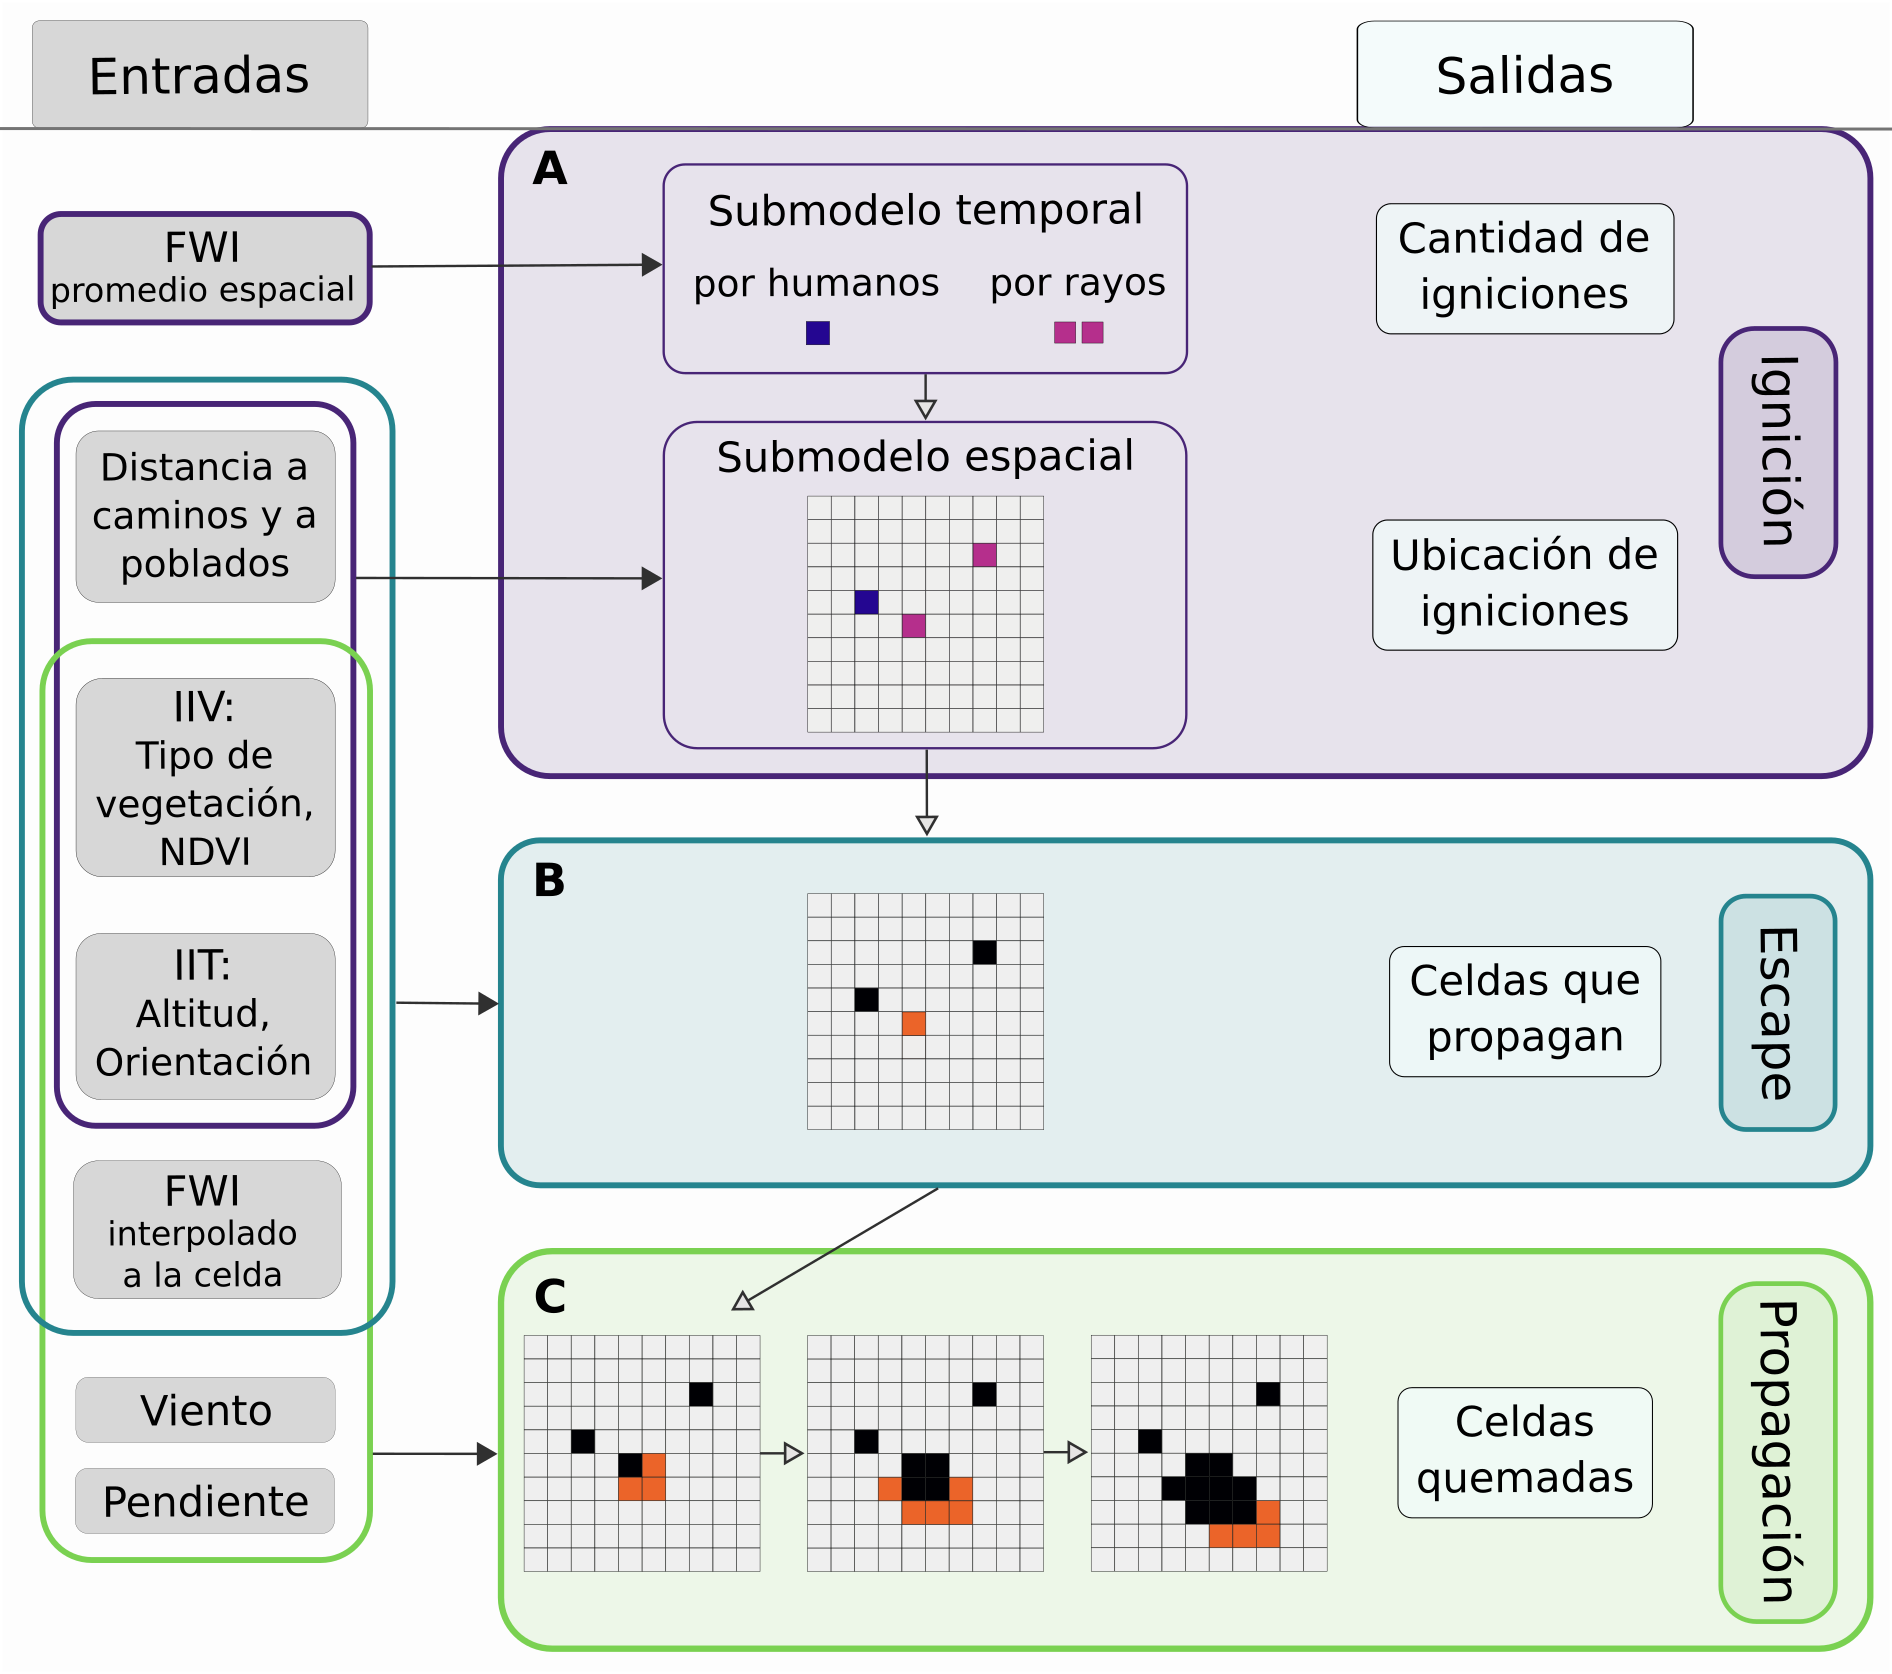
\includegraphics[width=13cm]{figuras/cap4/spread/esquema_modelos_fig2.png}
    \caption[Esquema de modelos de simulación.]{Esquema de los modelos de simulación. (A) El modelo de ignición está compuesto por dos submodelos: el temporal, que simula cuántas igniciones ocurren en toda el área de estudio por causa, en función del FWI promedio del área de estudio; y el espacial, que simula en qué celdas del paisaje ocurren dichas igniciones, en función de variables espaciales. La distancia a caminos y a poblados sólo regula la ubicación de igniciones humanas. El esquema ilustra un ejemplo con una ignición por humanos y dos por rayos. (B) El modelo de escape simula cuáles de las celdas en donde ocurrió ignición propagan fuego, sin importar su causa, en base a variables espaciales y al FWI interpolado a nivel de celda. En el esquema las celdas sin escape se representan en negro, y en naranja, una celda con escape. (C) El modelo de propagación simula el contagio desde las celdas en donde el fuego escapó, en función de variables espaciales y del FWI interpolado en cada celda. El esquema ilustra tres pasos de simulación, en donde el naranja representa las celdas encendidas en cada paso, que pasan a estar quemadas (negro) en el paso siguiente. La ignición, el escape, y la propagación se concatenan en cada quincena de simulación. Al simular el régimen de incendios, toda la rutina se repite a lo largo de todas las quincenas de un año, conformando una iteración. Dentro de una iteración, las celdas quemadas no pueden volver a quemarse. El NDVI se fija en el promedio del verano (dic-mar) en el año anterior al focal, por lo que no varía entre quincenas. El FWI varía entre quincenas pero tiene resolución espacial gruesa (24 km) comparado con las demás variables (30 m). IIV: Índice de Inflamabilidad de la Vegetación; IIT: Índice de Inflamabilidad por Topografía.}
    \label{fig:esquema}
\end{figure}


\FloatBarrier

\subsection{Proyecciones de la probabilidad de quema anual bajo escenarios de cambio climático}

Utilizando el simulador del régimen de incendios comparamos la probabilidad anual de quema en el PNNH para los períodos moderno (1998-2022) y las décadas de los 2040s (2040-2049) y 2090s (2090-2099). Para los períodos futuros utilizamos los escenarios SSP1-2.6, SSP2-4.5, SSP3-7.0 y SSP5-8.5 \citep{IPCC2023}. Estos escenarios representan trayectorias contrastantes de desarrollo socioeconómico y emisiones de gases de efecto invernadero. En el extremo más benévolo, el escenario SSP1-2.6 asume fuerte cooperación internacional, desarrollo sostenible y bajas emisiones. En el extremo más pesimista, el SSP5-8.5 representa un futuro con alta dependencia de combustibles fósiles y emisiones muy elevadas. Los escenarios intermedios (SSP2-4.5 y SSP3-7.0) reflejan trayectorias con esfuerzos de mitigación limitados o desigualdad regional acentuada. La elección de estos cuatro escenarios nos permitió capturar extremos y puntos intermedios del rango de proyecciones climáticas disponibles para el siglo XXI.

En total, simulamos el régimen de incendios bajo 9 condiciones climáticas (de ahora en más, experimentos): período moderno + 4 escenarios climáticos futuros $\times$ 2 décadas. Para calcular el IIV utilicé la capa de NDVI medio de 2021 (diciembre-marzo). Para disminuir el efecto borde simulamos las igniciones en un polígono extendido del PNNH, mediante un \textit{buffer} de 10 km (ver contornos en Fig.~\ref{fig:bp_models}E, \ref{fig:proj-2040}, y \ref{fig:proj-2090}), escalando la tasa de ignición a esa área. El área \textit{buffer} no fue tenida en cuenta a la hora de calcular la probabilidad de quema o la proporción quemada del paisaje, ya que esta presenta efecto borde.

En cada experimento caracterizamos el régimen de incendios utilizando el clima de varios años: 24 años en el período moderno y 10 años en los escenarios futuros. Para cada condición corrimos 2000 iteraciones del simulador anual, seleccionando el año al azar dentro del período de interés para extraer el raster de FWI. En los períodos futuros, para extraer el FWI del año sorteado, también seleccionamos el modelo climático y su realización. Para ello, en cada iteración sorteamos qué modelo climático usar en base a sus pesos, y una vez escogido el modelo seleccionamos al azar una de sus realizaciones. Los pesos de los modelos fueron determinados en función de su adecuación para representar el clima moderno en el PNNH (Apéndice~\ref{append:proj}). Utilizamos los modelos climáticos del CMIP6 y sus correspondientes realizaciones que presentaban proyecciones para los 4 escenarios (Tabla~\ref{tab:climtable}). Las proyecciones de FWI diarias fueron provistas por Fulden Batibeniz y Yann Quillcaille \citep{quilcaille2023FWI}. El procedimiento para calcular las anomalías de FWI quincenales a partir de proyecciones diarias se detalla en el Apéndice~\ref{append:proj}. 

Comparamos la probabilidad de quema anual simulada entre cada experimento de dos maneras. Primero, calculamos la proporción de celdas quemadas sobre el número de celdas quemables en el PNNH por iteración (año), y estimamos la proporción media a lo largo de las simulaciones por experimento. Para esto ajustamos un modelo Beta-Binomial, en donde la media y la dispersión variaron por experimento, a través del paquete \texttt{brms} \citep{brms}, utilizando las previas débilmente informativas definidas por defecto. Segundo, realizamos un mapa de probabilidad de quema anual por experimento, calculando la proporción de iteraciones en que se quemó cada celda del paisaje. Adicionalmente, evaluamos qué proporción del área quemada anual en el PNNH fue quemada por igniciones causadas por rayos. Para ello, utilizamos el conteo de celdas quemadas por rayos sobre el total de celdas quemadas (ignorando las simulaciones en donde no hubo incendios) para ajustar un modelo Beta-Binomial y así estimar la proporción por experimento.  

\section{Resultados}

\subsection{Ignición}

La tasa de ignición por quincena y km$^2$ aumentó de forma exponencial con el FWI, siendo este efecto ligeramente mayor para las igniciones por rayo que para las humanas (\cref{fig:igrate}). A su vez, las igniciones por rayo presentaron una tasa media más baja que las humanas y mayor dispersión.

\begin{figure}[htbp]
    \centering
    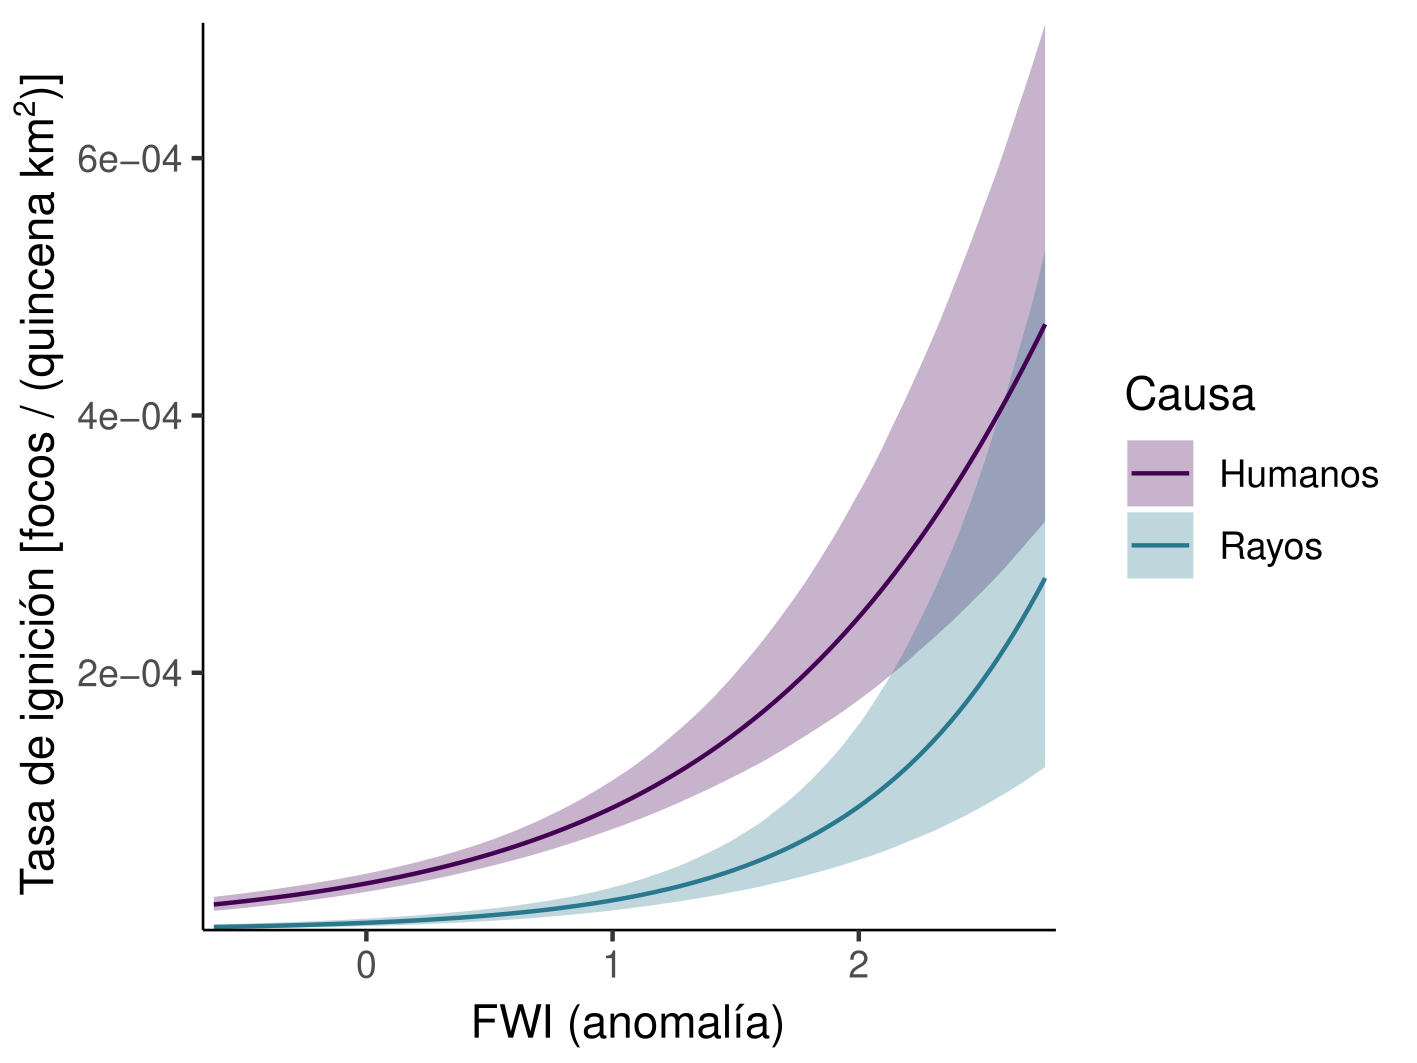
\includegraphics[width=12cm]{figuras/cap4/ignition/ignition_rate_fwi.png}
    \caption[Tasa de ignición en función del FWI.]{Tasa de ignición por quincena y km$^2$ en función de la anomalía de FWI para ambos tipos de causa. La línea y las bandas muestran la predicción de $\lambda$ (ver Ecuación~\ref{eq:igrate}), como la media y el intervalo de credibilidad del 95 \% de la distribución posterior.} 
    \label{fig:igrate}
\end{figure}

El submodelo espacial de ignición mostró un efecto considerable de la vegetación sobre la probabilidad relativa de ignición, siendo más marcado en las igniciones humanas (\cref{fig:ig_spat_veg}). De manera contraria, la topografía presentó un mayor efecto sobre las igniciones por rayos que sobre las humanas (\cref{fig:ig_spat_env}). En las igniciones humanas, las distancias a caminos y poblados presentaron efectos tan grandes que prácticamente dejaron sin efecto a las demás predictoras (Fig.~\ref{fig:ig_spat_env}, \ref{fig:bp_models}A). 

\begin{figure}[htbp]
    \centering
    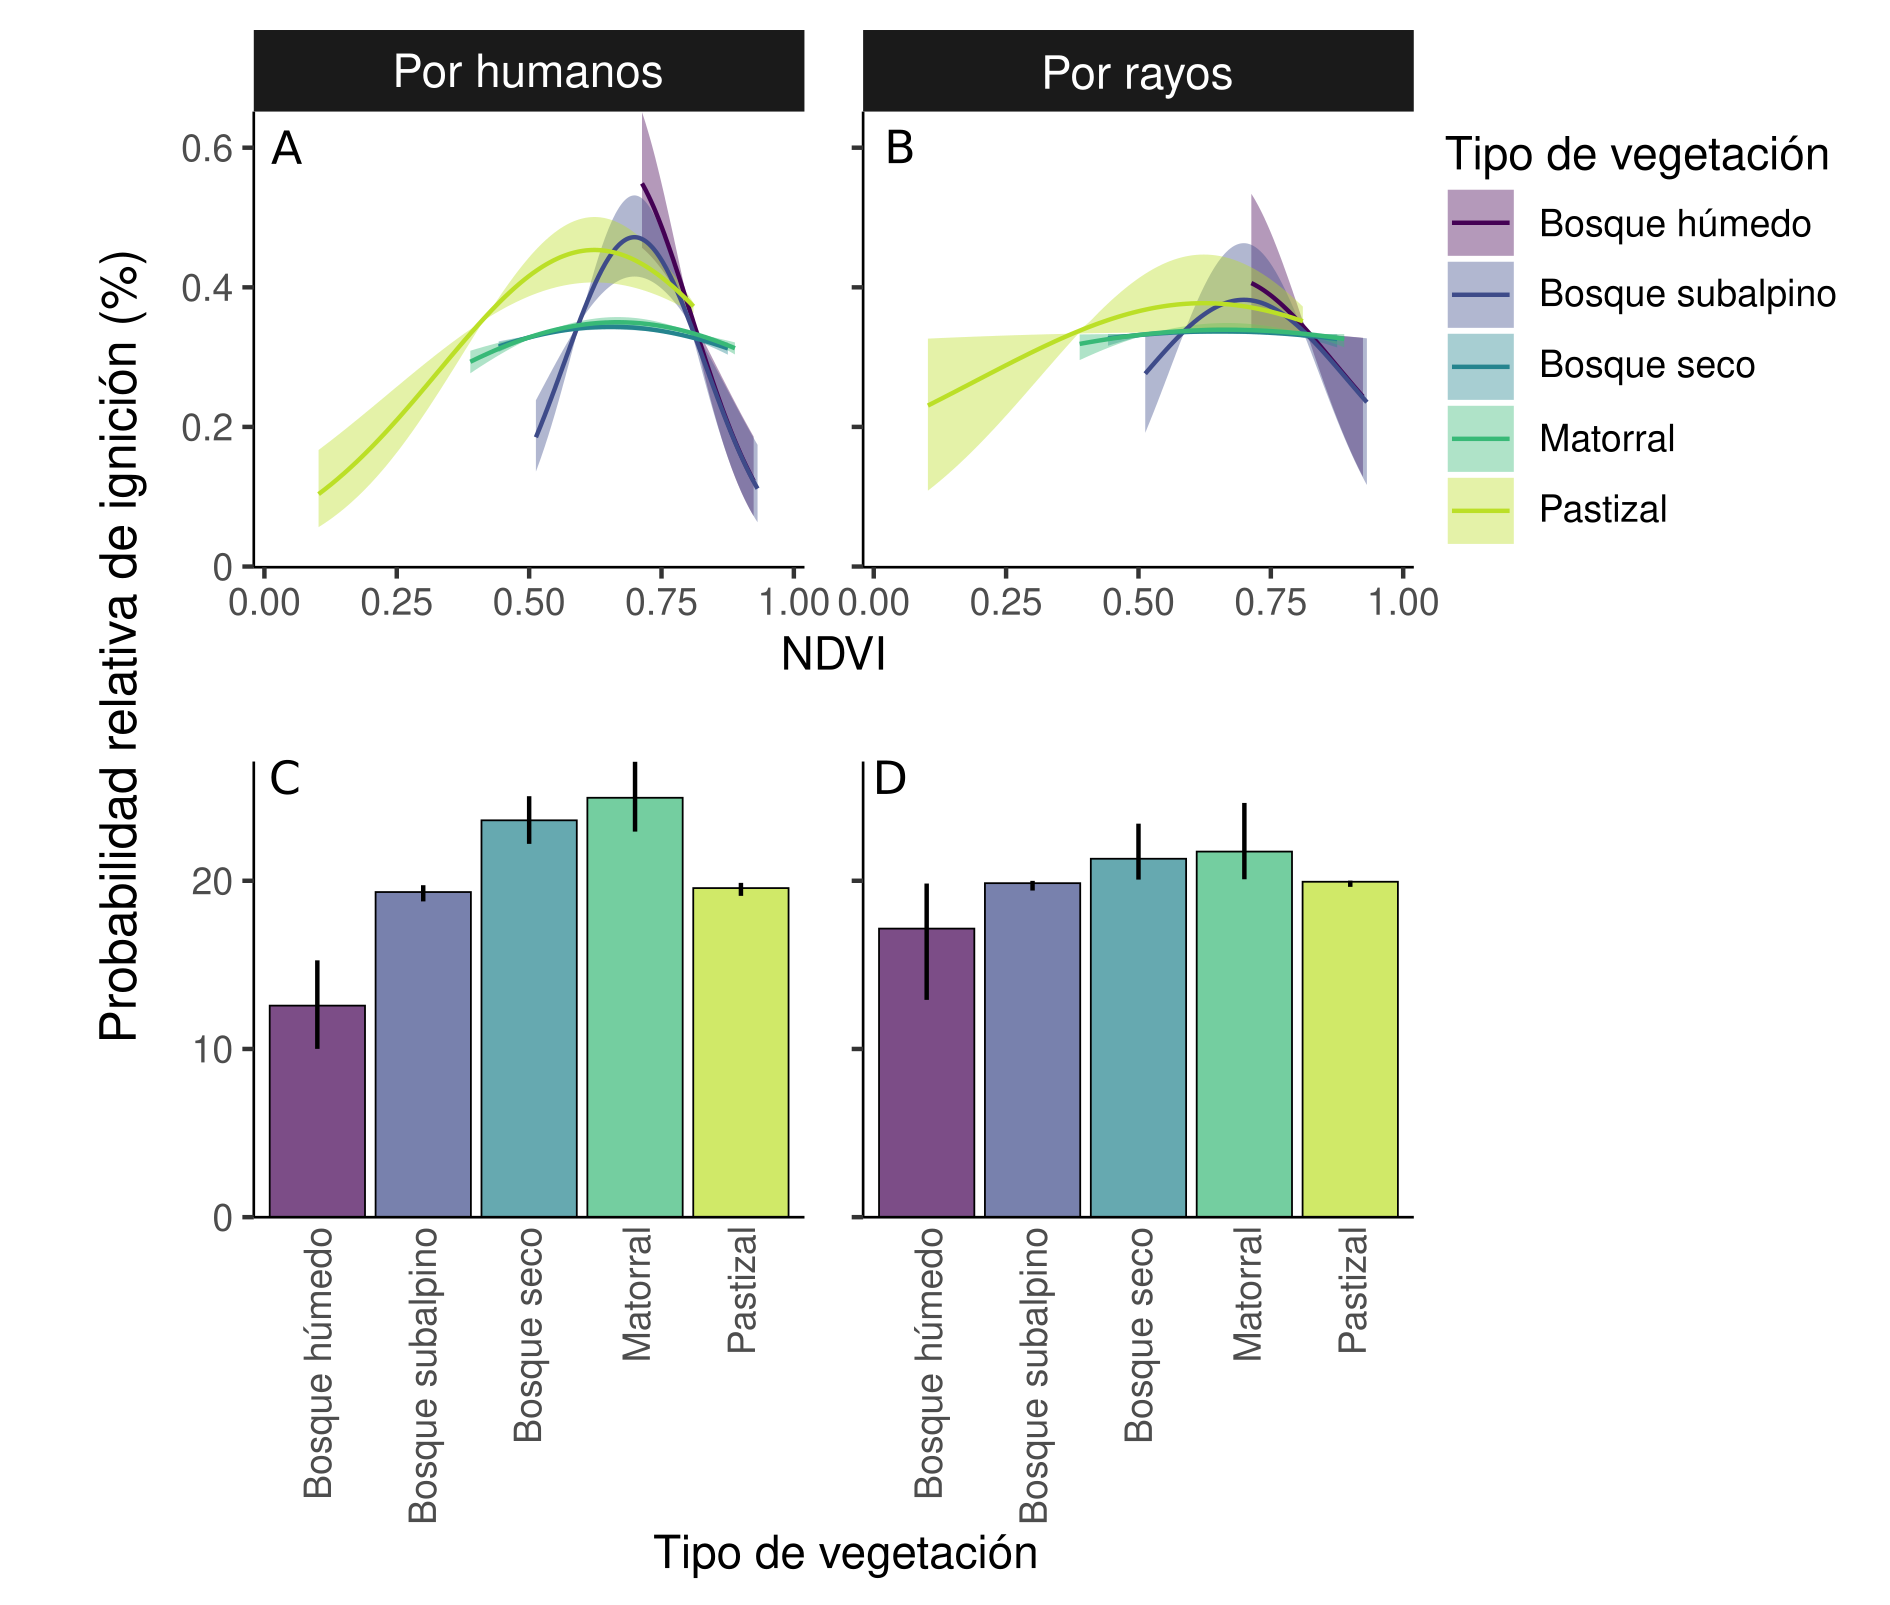
\includegraphics[width=16cm]{figuras/cap4/ignition/ignition_conditional_prob_veg.png}
    \caption[Probabilidad relativa de ignición en función de la vegetación.]{Probabilidad relativa de ignición función del NDVI por tipo de vegetación (A, B) y en función del tipo de vegetación (C, D), separando por causa, según el submodelo espacial de ignición. Las curvas fueron calculadas utilizando una secuencia regular de 300 valores de NDVI por tipo de vegetación, de forma tal que la suma de sus valores es 100 \%. Los valores de las demás predictoras fueron fijadas en sus medias. En los paneles de arriba, los valores son sólo comparables dentro de cada tipo de vegetación. Los paneles de abajo permiten comparar entre tipos de vegetación; en este caso el NDVI fue fijado en la media para cada tipo de vegetación. Las curvas (arriba) y barras (abajo) representan la media de la distribución posterior de $\theta$ (Ecuación \ref{eq:igspat}), con sus respectivos intervalos de credibilidad del 95 \% a modo de bandas o líneas verticales.} 
    \label{fig:ig_spat_veg}
\end{figure}

% Figura grande ocupando 2 páginas (figura y leyenda)
\begin{figure}[b!]
  \centering 
  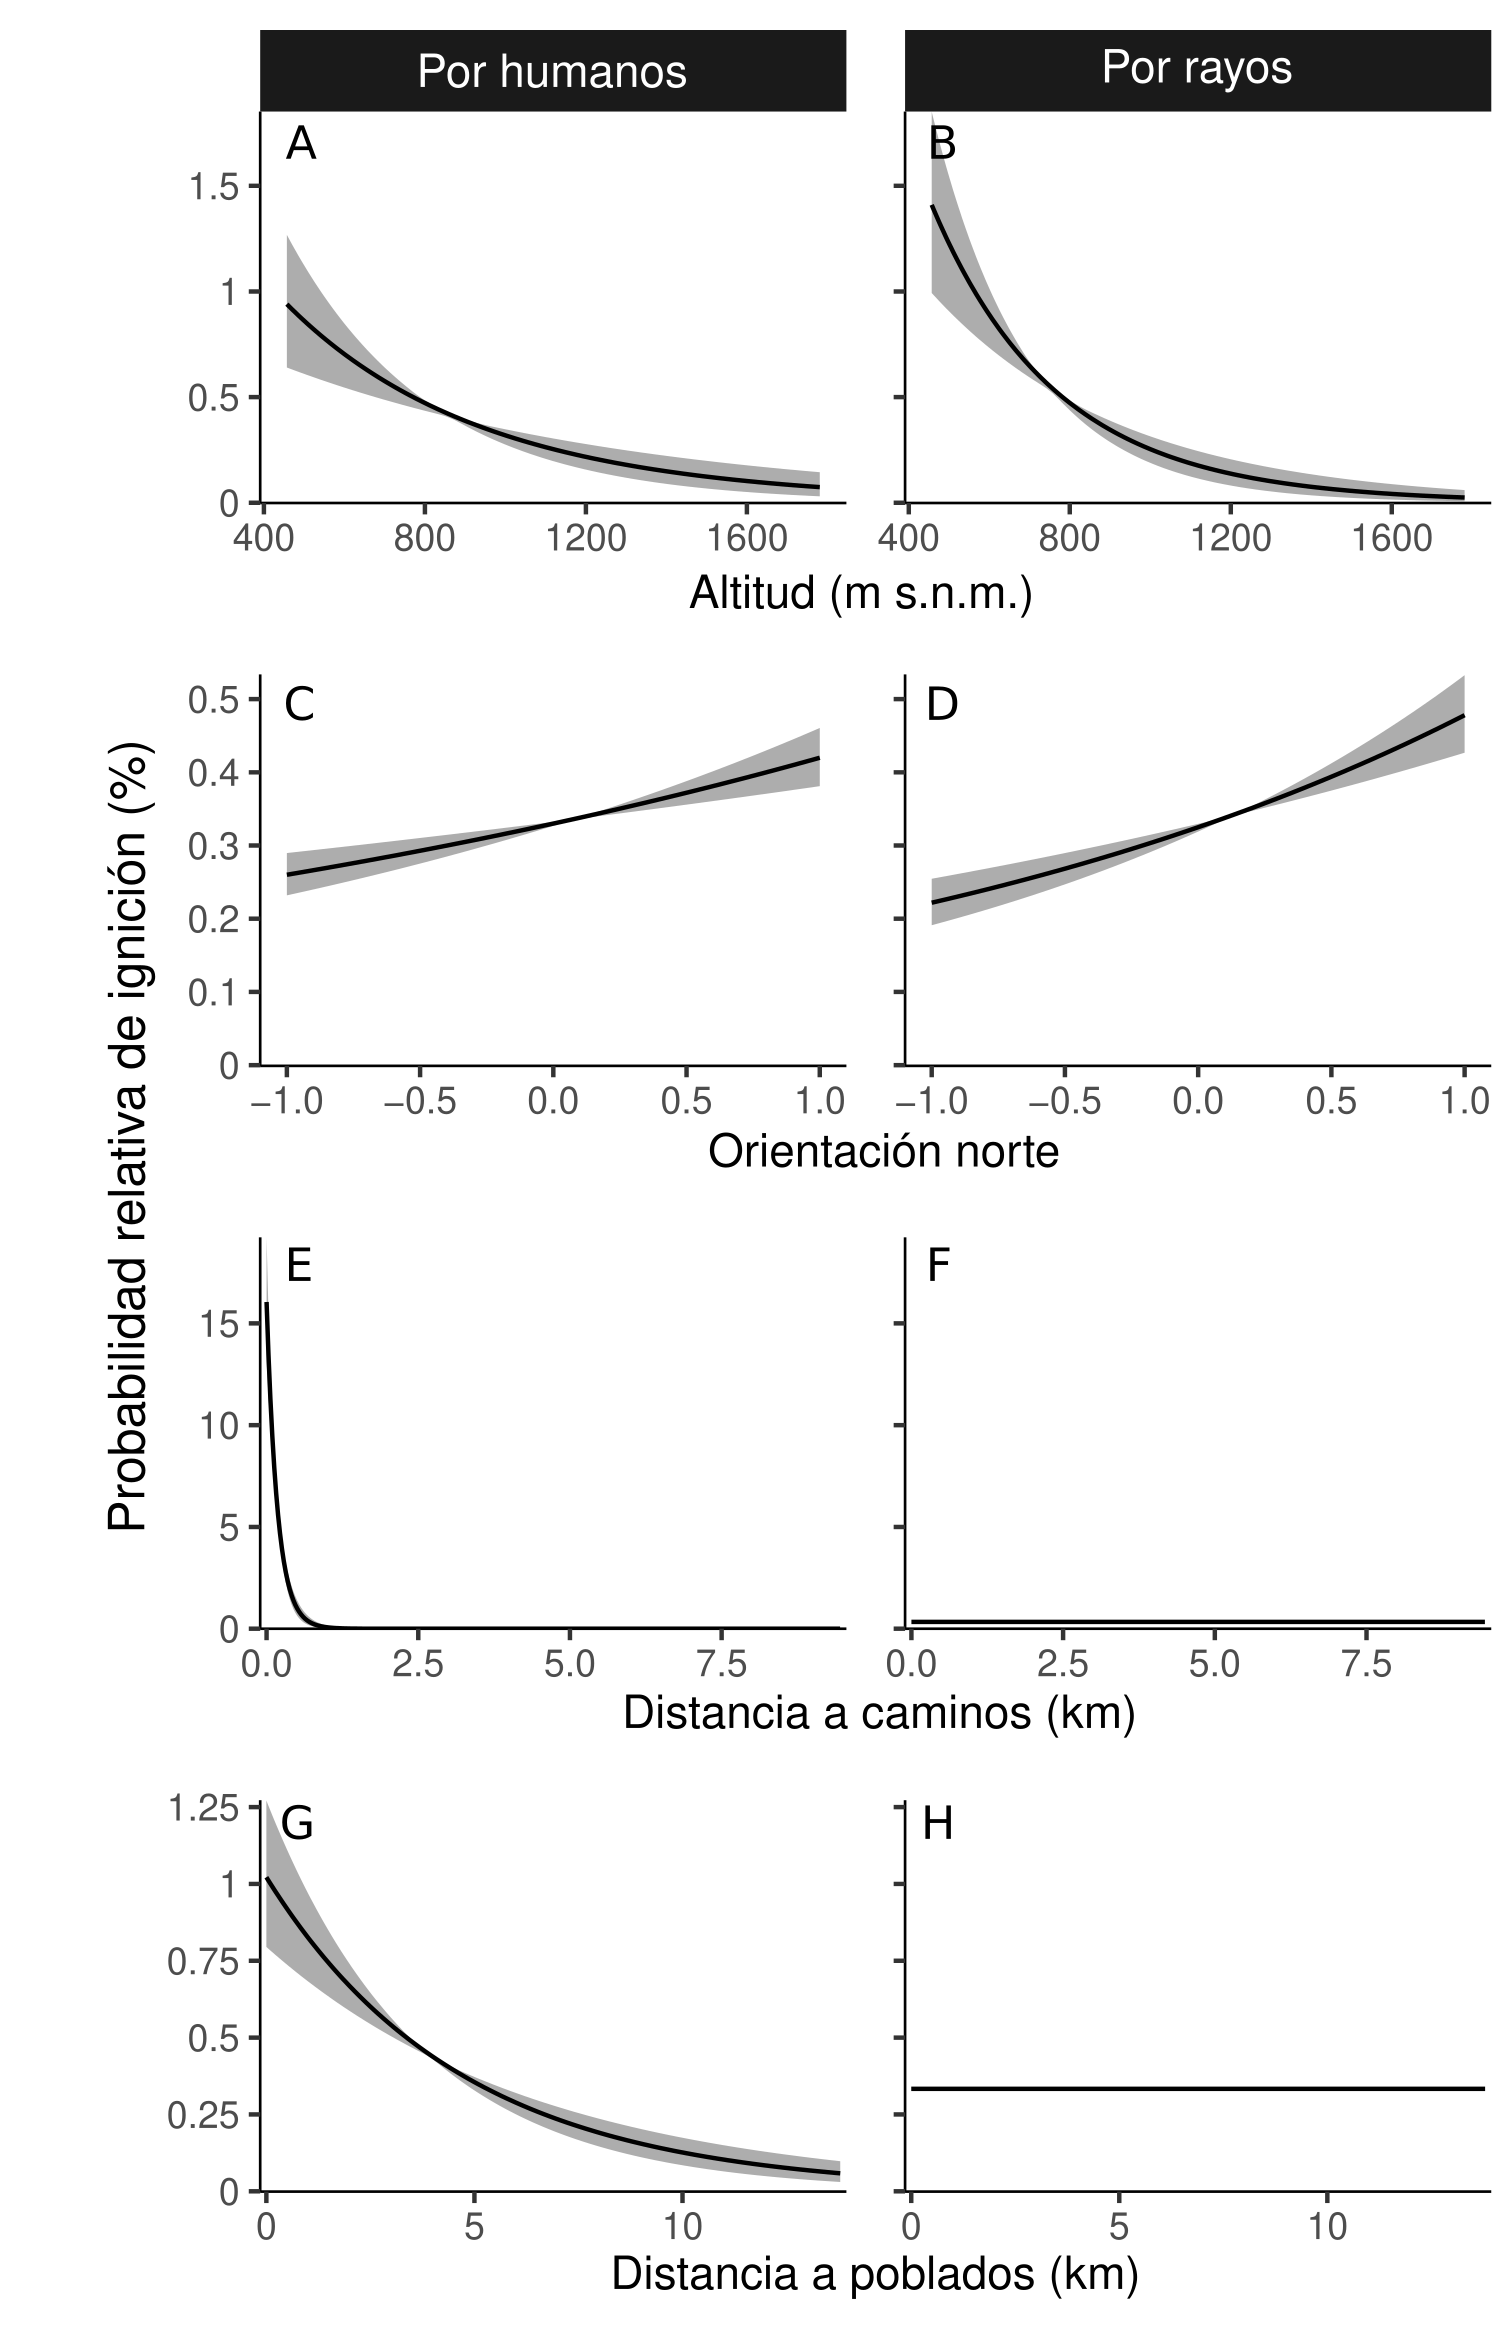
\includegraphics[width=0.8\textwidth]{figuras/cap4/ignition/ignition_conditional_prob_environment.png}
  \caption[Probabilidad relativa de ignición en función de variables ambientales.]{Probabilidad relativa de ignición en función de variables topográfias e indicadoras de influencia humana, separando por causa, según el submodelo espacial de ignición. Las curvas fueron calculadas utilizando una secuencia regular de 300 valores de cada predictora, de forma tal que la suma de sus valores es 100 \%, y las covariables no focales fueron fijadas en sus medias. Las líneas y bandas representan la media de la distribución posterior de $\theta$ (Ecuación \ref{eq:igspat}) y su intervalo de credibilidad del 95 \%, respectivamente.}
  \label{fig:ig_spat_env}
\end{figure}

\FloatBarrier % no ignition images below

\subsection{Escape}

La probabilidad de escape presentó variaciones relativamente pequeñas en función de la mayor parte de las predictoras, a excepción de las distancias a caminos y a poblados, las cuales aumentaron la probabilidad de escape (Fig.~\ref{fig:escape}). Dado que estas dos variables están correlacionadas en el paisaje (pero no en el set de datos de igniciones), su efecto conjunto puede ser considerable (Fig.~\ref{fig:bp_models}C).

% Figura grande ocupando página entera, para ubicar leyenda en la pág siguiente
\begin{figure}[b!]
  \centering 
  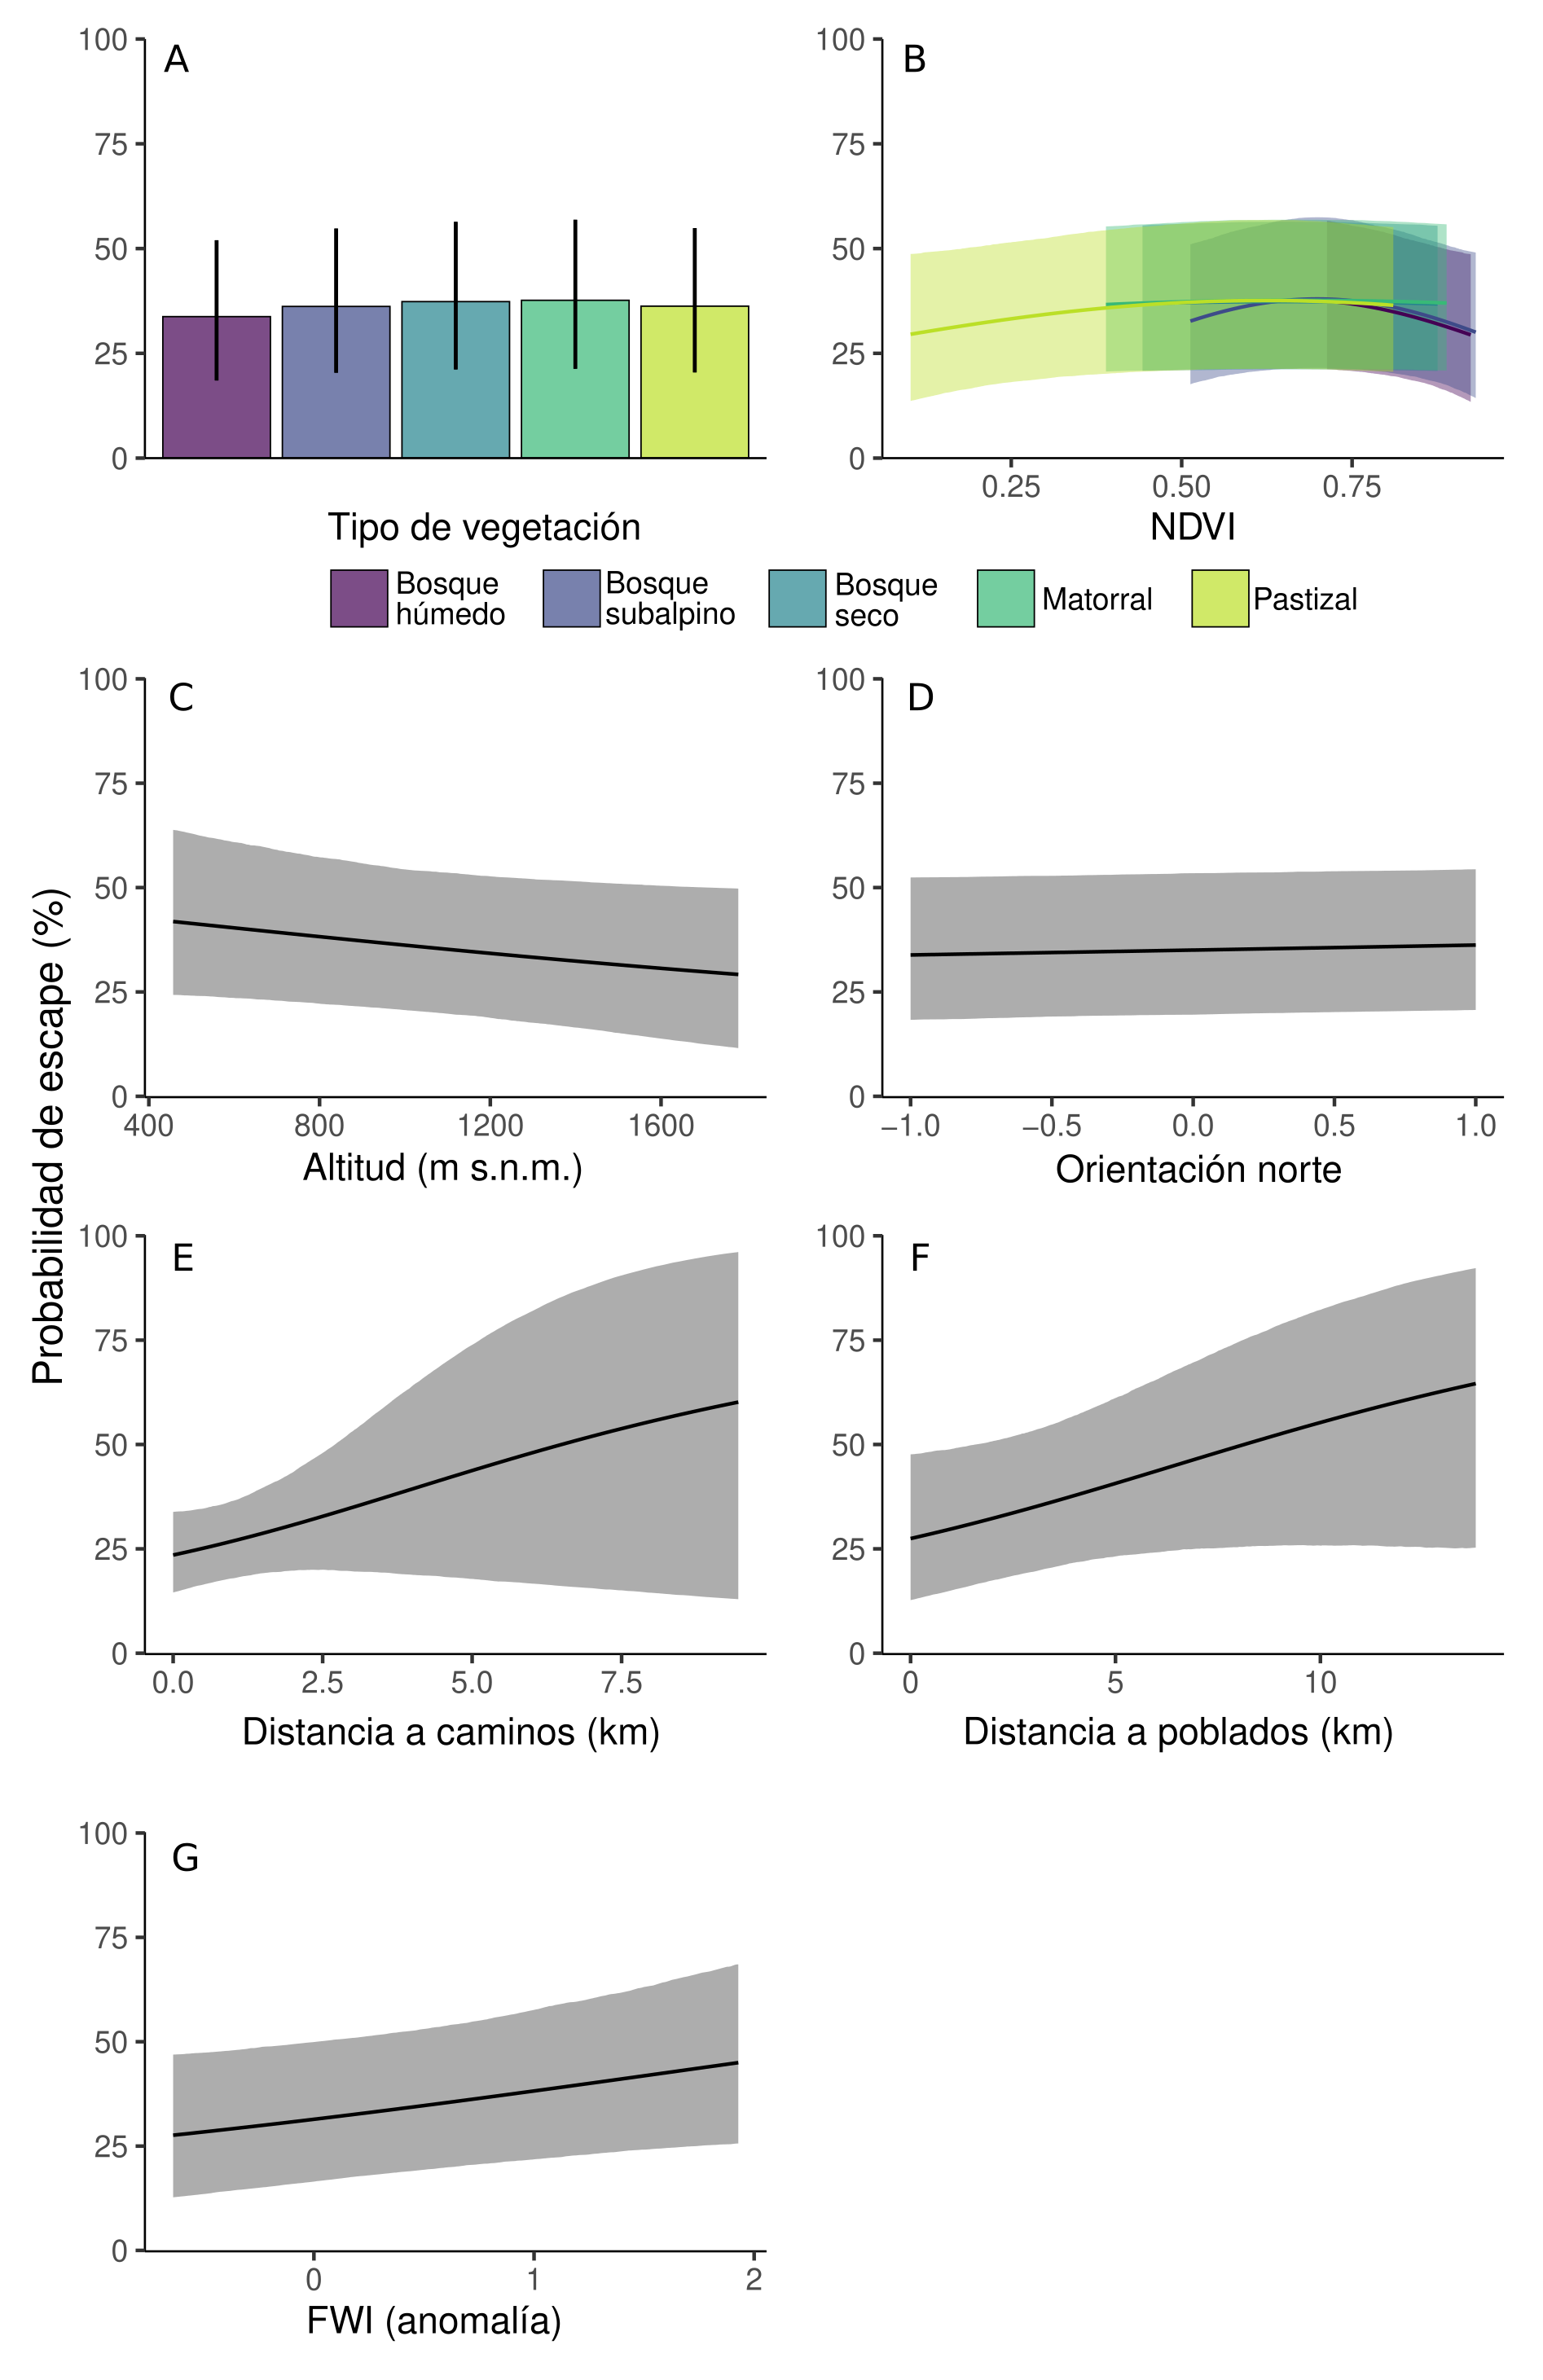
\includegraphics[height=0.95\textheight]{figuras/cap4/escape/escape_effects.png}
  \caption[Probabilidad de escape en función de las variables predictoras.]{(Leyenda en la página siguiente.)}
  \label{fig:escape}
\end{figure}

% leyenda en la página siguiente
\begin{figure}[p]
  \contcaption{(en la página anterior). Probabilidad de escape en función de las predictoras. Todas las predictoras no focales fueron fijadas en sus medias para calcular predicciones parciales. En el caso del FWI utilizamos la media acumulada en los datos de ignición (0.57). Las líneas y bandas representan la media de la distribución posterior de $\theta$ (Ecuación \ref{eq:escape}) y su intervalo de credibilidad del 95 \%, respectivamente.} 
\end{figure}

\FloatBarrier % no escape images below

\subsection{Propagación}

La probabilidad de propagación varió principalmente en función del viento y la pendiente, con los índices de inflamabilidad (vegetación y topografía) presentando efectos moderados (Fig.~\ref{fig:spread-curves} y \ref{fig:spread-curves-x}). Los parámetros de propagación presentaron una notable variabilidad no explicada entre incendios; sin embargo, algunos de ellos también variaron notablemente en función del FWI. A mayor FWI disminuyó el efecto de la pendiente y aumentó el efecto del viento (\cref{fig:spread-params}). Además de estos efectos contrapuestos del FWI sobre los efectos medios de la pendiente y el viento, el modelo estimó una correlación negativa entre estos efectos ($\beta_3$ y $\beta_4$ en la Ecuación~\ref{eq:datamodel}), reflejando que los incendios tienden a ser dominados por pendiente o por viento (\cref{fig:spread-corr}). Por otro lado, los pasos de simulación aumentaron considerablemente con el FWI, y mostraron una correlación positiva con el efecto del viento (Fig.~\ref{fig:spread-curves} y \ref{fig:spread-corr}). El efecto de la topografía (efecto no direccional de altitud y orientación; IIT) presentó un pequeño aumento en función del FWI, mientras que el efecto de la vegetación (IIV) no varió con el FWI (Fig.~\ref{fig:spread-curves} y \ref{fig:spread-veg-effects}, Apéndice~\ref{append:spread-veg-effects}).

Utilizando los parámetros estimados para cada incendio, los fuegos simulados tuvieron un solapamiento relativamente alto con los observados (\cref{fig:spread-ov}), pero este valor decreció al usar parámetros simulados desde la distribución estimada. Esto indica que la parte determinística del modelo de propagación no puede representar bien las particularidades de cada incendio, sino que gran parte de la variación se asocia a aspectos no considerados (e.g., condiciones atmosféricas a escala temporal fina, o particularidades del combate del fuego). Además, sin contar con datos de velocidad del viento para cada incendio, el modelo estima su efecto, que representa la velocidad promedio. Entonces, para poder simular fuegos similares a los ocurridos, necesitamos usar la velocidad estimada ($\beta_4$ en la Ecuación~\ref{eq:datamodel}); si simulamos velocidades a partir de la distribución estimada, los incendios simulados difieren del observado. Esto resulta esperable, ya que el viento es un factor determinante de la propagación \citep{rothermel_mathematical_1972}. El tamaño de los incendios simulados con los parámetros ajustados fue similar al tamaño observado (\cref{fig:spread-q}A), pero utilizando parámetros simulados, la discrepancia fue considerable (\cref{fig:spread-q}B). Pero a pesar de que el modelo de propagación no puede reproducir fuegos particulares salvo que se utilicen parámetros ajustados a cada incendio, el mismo puede simular incendios con una distribución de tamaño similar. Es decir, puede simular incendios con características similares a los observados. Aún así, utilizando parámetros simulados el modelo subestima la variación en tamaño de los incendios observados (nótese cómo el cociente decrece desde valores $>1$ a $<1$ en la Fig.~\ref{fig:spread-q}B).

\begin{figure}[htbp]
  \centering 
  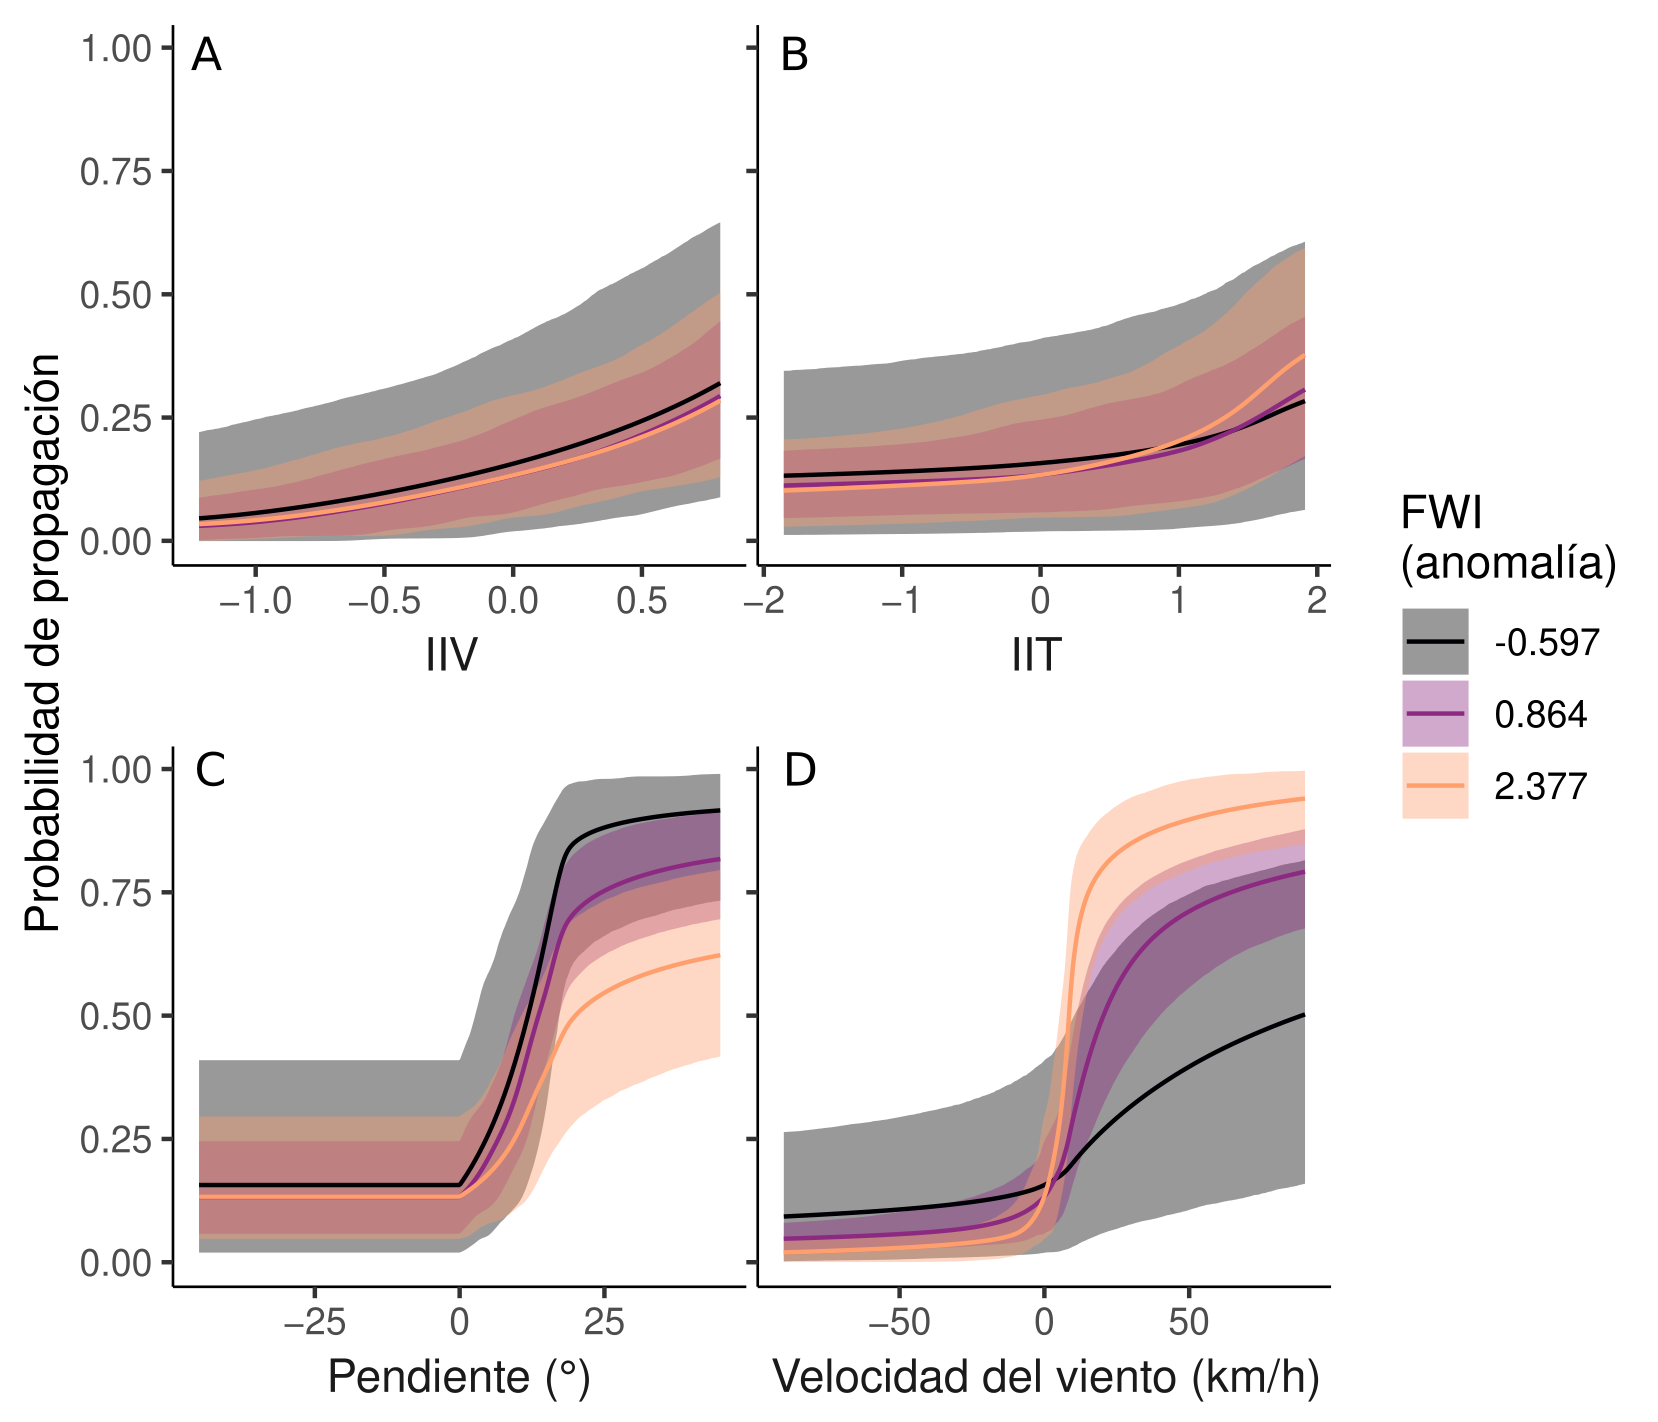
\includegraphics[width=14cm]{figuras/cap4/spread/spread_prob_curves.png}
  \caption[Probabilidad de propagación en función de la vegetación, topografía, pendiente y velocidad del viento.]{Probabilidad de propagación en función las predictoras, para tres valores contrastantes de FWI acumulado (media y percentiles 2.5 y 97.5 \% de los incendios mapeados en el Capítulo~\ref{cap:patrones}). Cada curva representa el promedio de la distribución de parámetros, calculados mediante simulación. Las líneas y bandas representan la media y el intervalo de credibilidad del 95 \% de la distribución posterior. IIV: Índice de Inflamabilidad de la Vegetación; IIT: Índice de Inflamabilidad por Topografía. Estos índices son adimensionales, y valores más altos indican mayor inflamabilidad. (Ver sus definiciones en la Ecuación~\ref{eq:FI}).}
  \label{fig:spread-curves}
\end{figure}

\begin{figure}[htbp]
  \centering 
  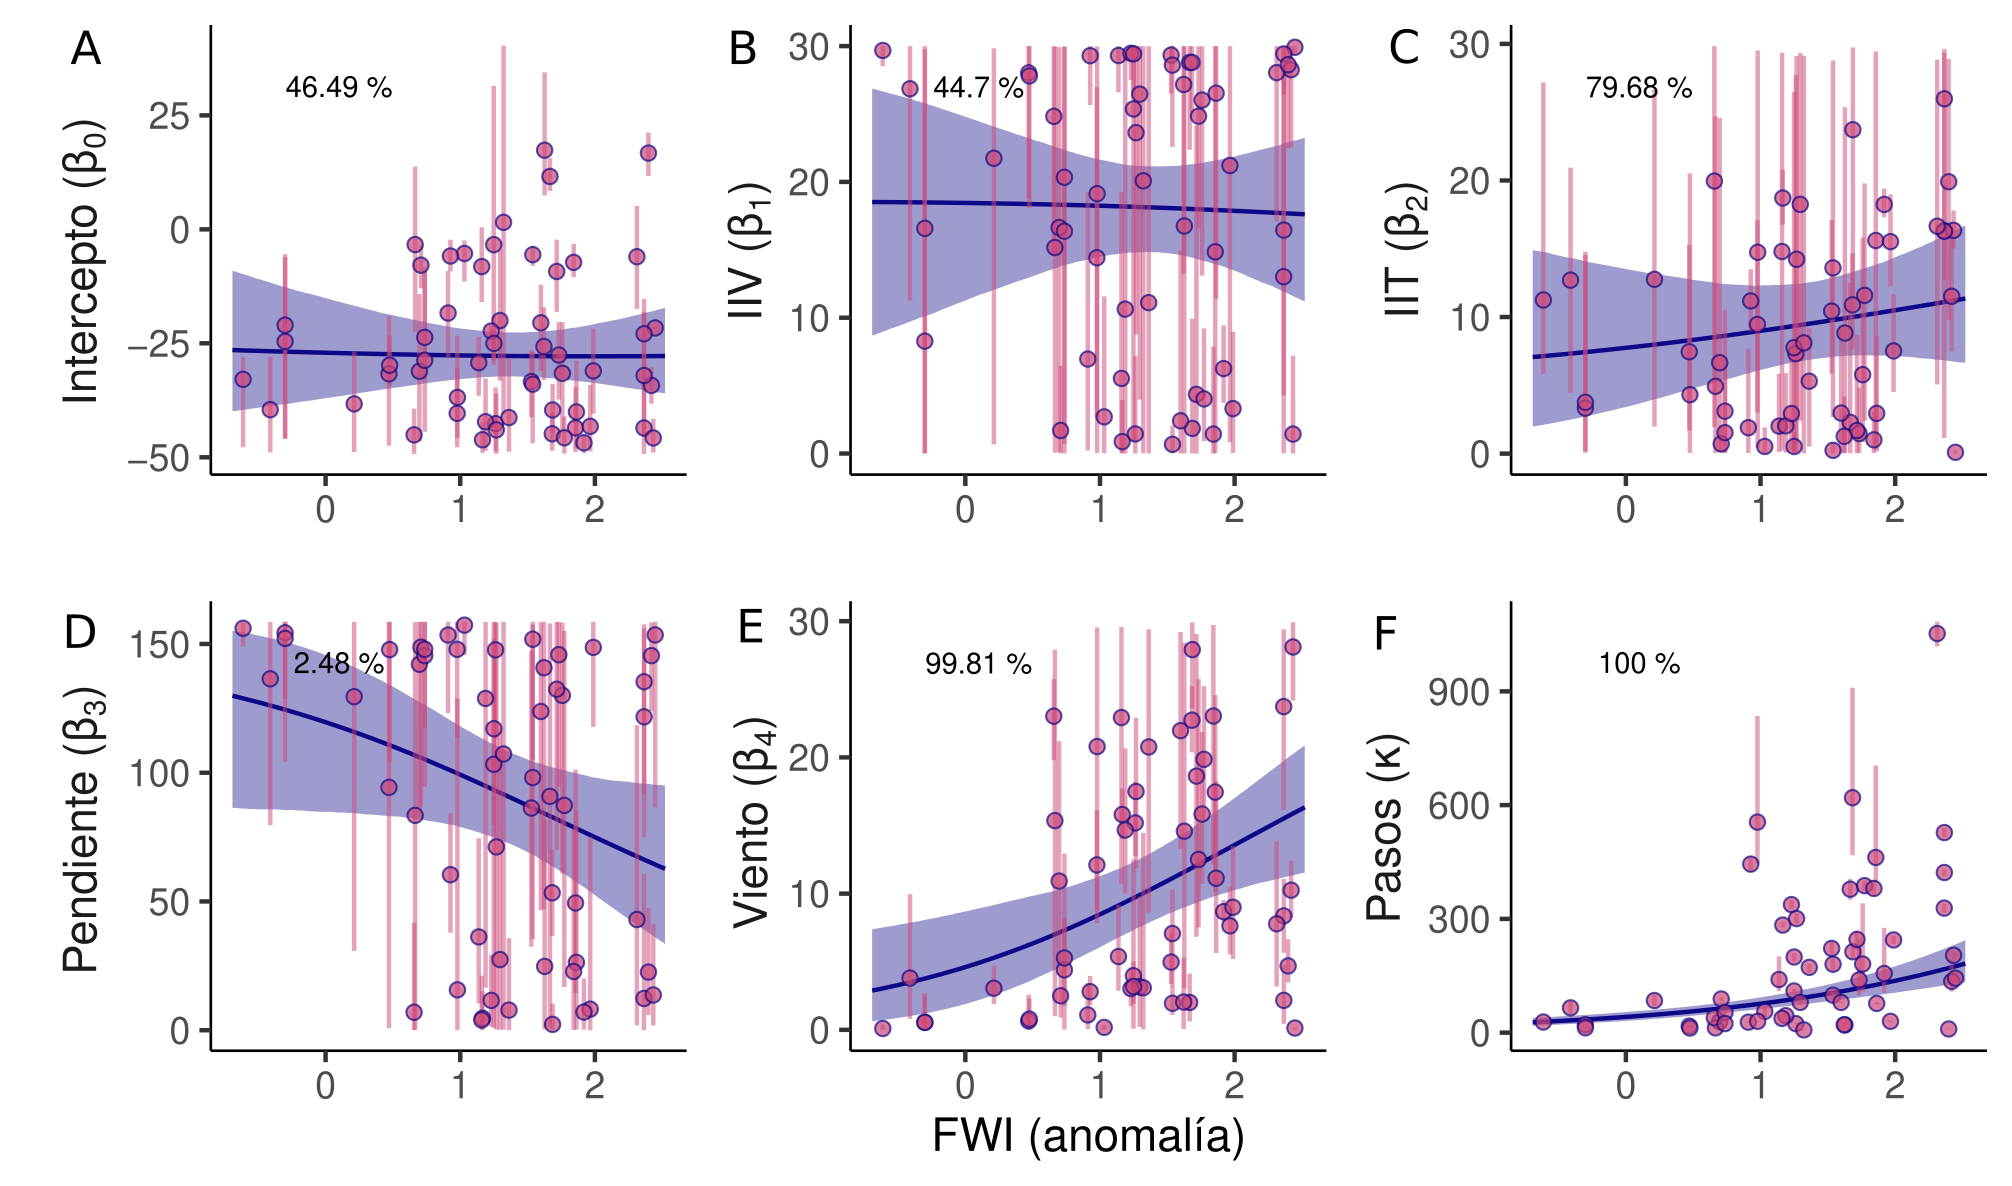
\includegraphics[width=\textwidth]{figuras/cap4/spread/params_fwi_regression.png}
  \caption[Parámetros de propagación en función del FWI.]{Parámetros de propagación en función del FWI. Las curvas y bandas muestran la media de los efectos aleatorios (como media e intervalo del 95 \% de su distribución posterior), mientas que los puntos y líneas verticales muestran el parámetro estimado para cada incendio. Los porcentajes dentro de cada panel indican la probabilidad de que la media aumente en función del FWI (0 \% indica completa certeza sobre un efecto negativo; 50 \% indica incertidumbre total sobre el signo del efecto, y 100 \% indica certeza completa de un efecto positivo). Los pasos ($\kappa$) indican el número máximo de pasos de simulación (ver Ecuación~\ref{eq:datamodel}).}
  \label{fig:spread-params}
\end{figure}

\begin{figure}[htbp]
  \centering 
  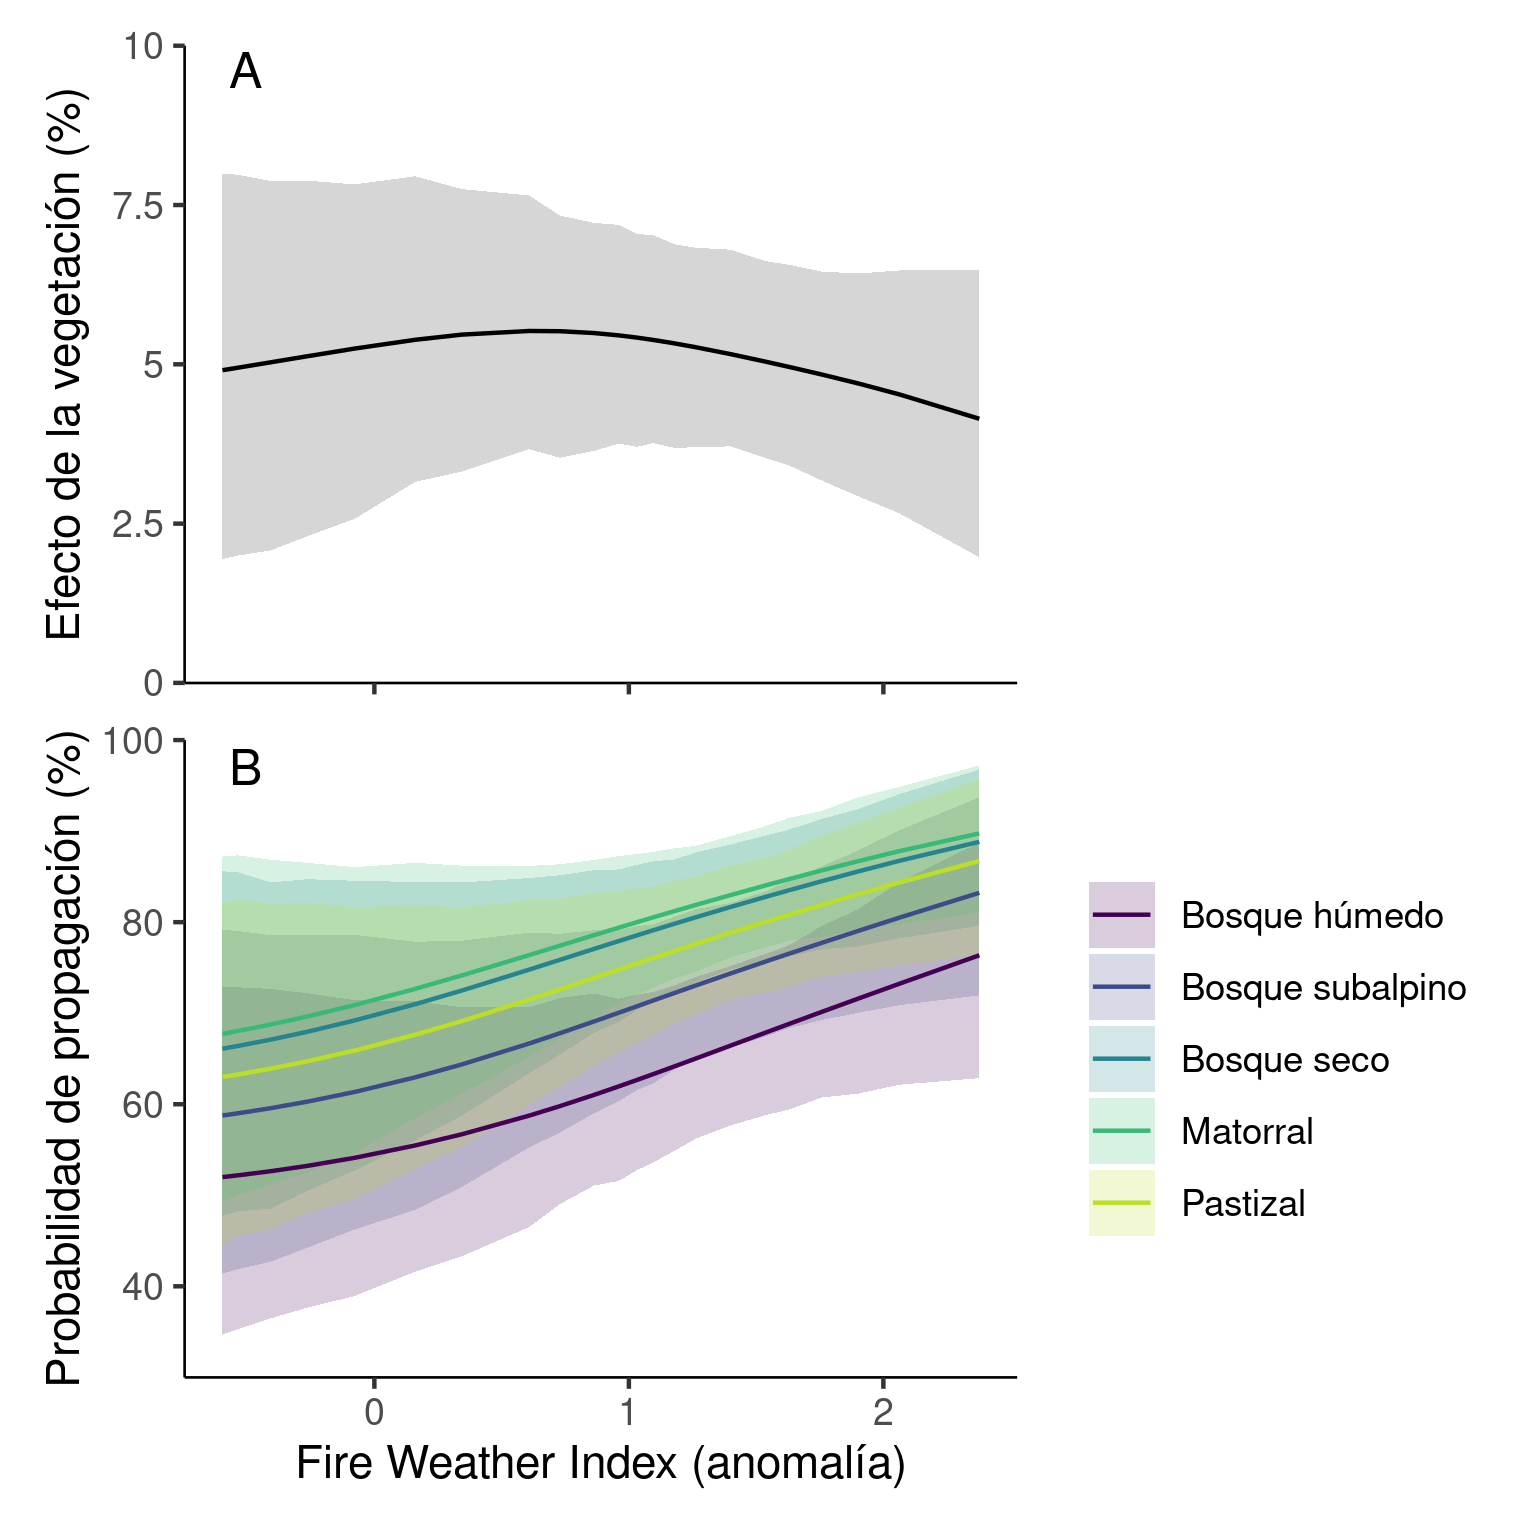
\includegraphics[width=13cm]{figuras/cap4/spread/vegetation_effects_fwi.png}
  \caption[Efecto de la vegetación sobre la probabilidad de propagación en función del FWI.]{(A) Efecto del tipo de vegetación sobre la probabilidad de propagación en función del FWI, calculado como el desvío absoluto medio entre las probabilidades estimadas para los cinco tipos de vegetación, mostradas en (B). (B) Probabilidad de propagación en función del FWI por tipo de vegetación. Para comparar la probabilidad de propagación entre tipos de vegetación, fijamos la altitud en 900 m s.n.m., la orientación en 90° (componente norte = 0), y marginalizamos sobre la distribución de NDVI, pendiente y velocidad del viento en el PNNH (detalles en el Apéndice~\ref{append:spread-veg-effects}).}
  \label{fig:spread-veg-effects}
\end{figure}

% agrandar márgenes de página
\newgeometry{top=0.5cm, bottom=0.5cm, left=1cm, right=1cm}

% Figura grande ocupando página entera, para ubicar leyenda en la pág siguiente
\begin{figure}[b!]
  \centering 
  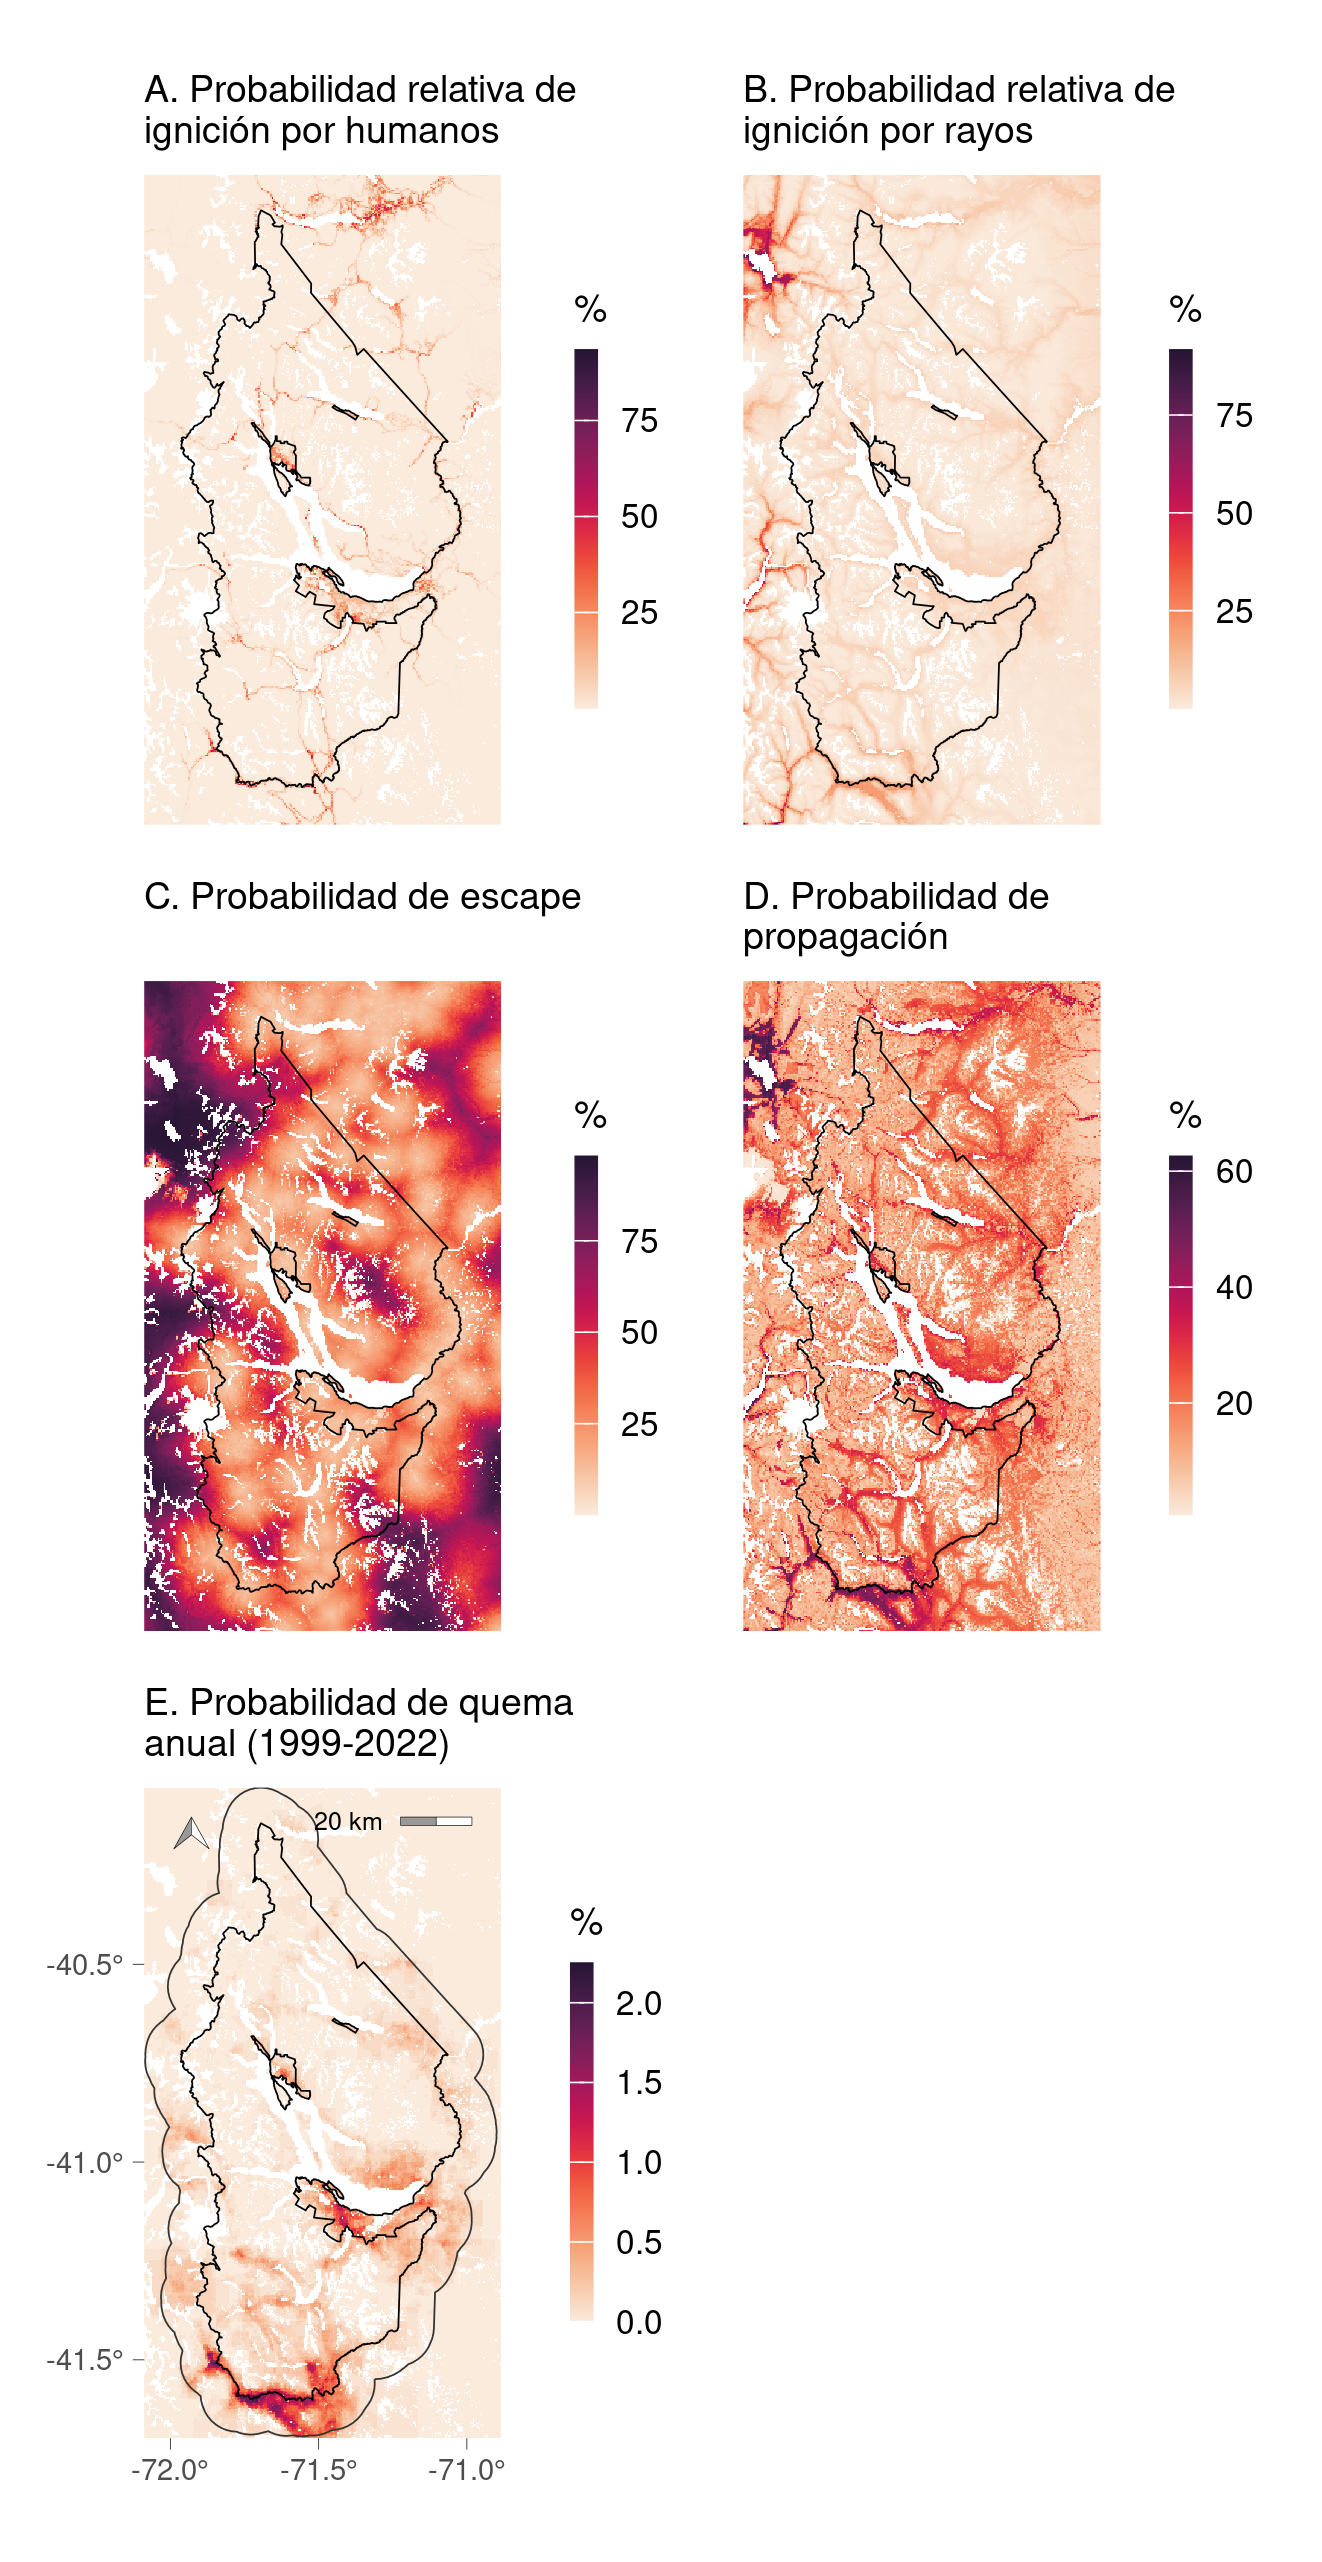
\includegraphics[width=13.8cm]{figuras/cap4/projections/burn_prob_models_modern.png}
  \caption[Probabilidad de ignición, escape, propagación y quema en el PNNH.]{(Leyenda en la página siguiente.)}
  \label{fig:bp_models}
\end{figure}

% restaurar márgenes de página
\restoregeometry


% leyenda en la página siguiente
\begin{figure}[p]
  \contcaption{(en la página anterior). Probabilidad de ignición, escape, propagación y quema en el PNNH. Las probabilidades de ignición (A, B), escape (C) y propagación (D) son predicciones de sus respectivos modelos, tomando el promedio de la distribución posterior, y fueron calculadas fijando el FWI en el promedio de la base de datos de focos. Para calcular la probabilidad de propagación se fijó la velocidad del viento en 14.4 km/h. La probabilidad de quema anual (E) se obtuvo simulando el régimen de incendios por 2000 iteraciones, integrando los tres modelos. El contorno alrededor del parque señala el área donde se simularon las igniciones, para evitar subestimar la probabilidad de quema en los bordes del PNNH.} 
\end{figure}

\FloatBarrier % no spread images below

\subsection{Proyecciones de la probabilidad de quema anual bajo escenarios de cambio climático}

La proporción quemada anual en el PNNH presentó una notable variación entre períodos y escenarios climáticos (Fig.~\ref{fig:proj-means}A, Tabla~\ref{tab:burn-prob-means}). Para los 2040s se espera que la proporción aumente en un factor de entre $\approx$ 2 y $\approx$ 2.6 con respecto al período 1999-2022, alcanzando valores entre el 0.2 y el 0.25 \% anual, según el escenario. Nótese que este valor es el mismo que encontramos para 1999-2022 en una región más amplia (Sección~\ref{cap3:patrones-regimen}), que incluye zonas con mayor incidencia del fuego que el PNNH. Para los 2090s se esperan aumentos mucho mayores en general y mucho más variables entre escenarios, con la proporción quemada anual variando entre 0.13 y 2.97 \%, lo cual representa aumentos en factores de entre 1.36 y 31.17 para los escenarios más optimista y pesimista, respectivamente (SSP1-2.6 vs. SSP5-8.5). En ambos períodos futuros y bajo todos los escenarios climáticos se espera que la proporción quemada anual media aumente, y únicamente para el escenario SSP1-2.6 en 2090-2099 se espera un aumento menor al doble con respecto al período 1999-2022 (Fig.~\ref{fig:proj-means}, Tabla~\ref{tab:burn-prob-means}). 

Más allá de las diferencias en proporción quemada anual media entre experimentos, cabe destacar que la proporción quemada varió notablemente entre años simulados, y a su vez, distintos experimentos presentaron contrastante variabilidad (Fig.~\ref{fig:proj-cdf}). Los percentiles del 95 \% de la distribución de proporción quemada anual variaron entre 0.45 \% para 1999-2022 y 14.47 \% para 2090-2099 bajo SSP5-8.5, y los máximos, entre 8.08 \% y 60.29 \%, respectivamente. 

La proporción quemada por rayos sobre el total quemado anualmente en el PNNH presentó variaciones mucho menores que la proporción quemada del paisaje, presentando aumentos marcados únicamente para el período 2090-2099 en los escenarios más pesimistas (SSP3-7.0 y SSP5-8.5, Fig.~\ref{fig:proj-means}B, Tabla~\ref{tab:burn-prob-means}). Bajo esas condiciones, se esperaría que la contribución relativa de los rayos al área quemada aumente al $\approx$ 34 \%, comparado con el $\approx$ 25 \% estimado para 1999-2022. 

Si bien la proporción quemada anual varió notablemente entre escenarios, la probabilidad de quema anual a nivel de píxel mantuvo un patrón espacial similar entre experimentos (Fig.~\ref{fig:bp_models}E, \ref{fig:proj-2040}, y \ref{fig:proj-2090}). Esto indica que la mayor incidencia del fuego no afectaría cualitativamente la disposición espacial de zonas con mayor y menor incidencia de fuego. La zona de mayor probabilidad de quema fue el valle del Manso Inferior, al sur del PNNH, debido a su baja altitud ($\approx$ 400 m s.n.m.) y a la presencia de caminos y poblados. Otras zonas de alta probabilidad de quema son los alrededores de Bariloche y Dina Huapi, que también presentan altitud relativamente baja y presencia humana. Más allá de estas zonas, se evidenció un notable efecto de la altitud, con los valles más extensos y profundos mostrando una relativamente alta probabilidad de quema luego de las zonas arriba mencionadas.

\begin{figure}[htbp]
  \centering 
  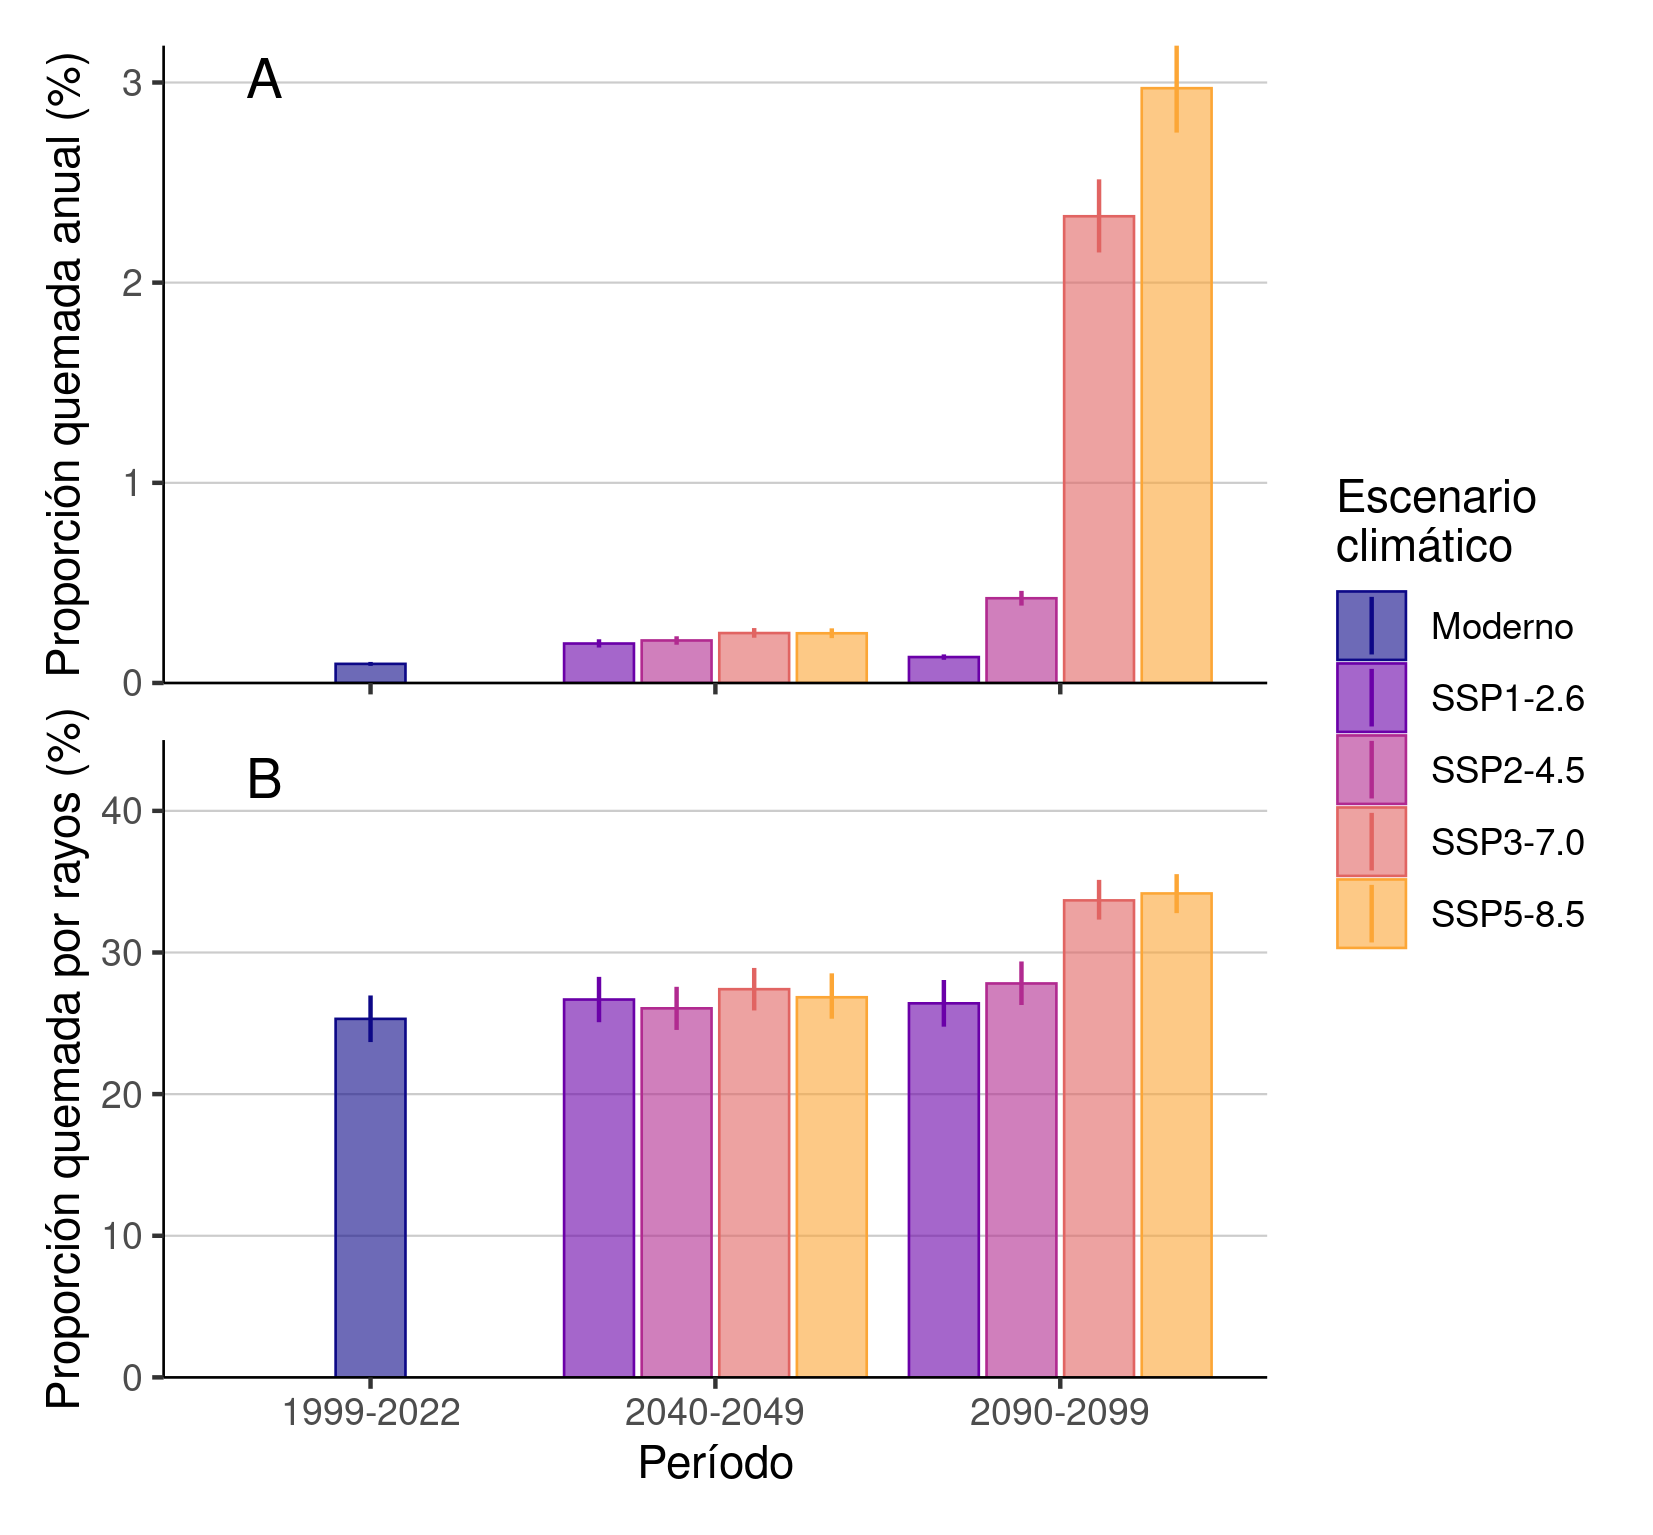
\includegraphics[width=14cm]{figuras/cap4/projections/burn_prob_light_mean_comparison.png}
  \caption[Proporción quemada del PNNH bajo escenarios de clima actual y futuro.]{(A) Proporción quemada de la superficie quemable del PNNH por experimento, y (B) fracción quemada por rayos de la superficie quemada en el PNNH. Las barras muestran la media de la distribución posterior, y las líneas, el intervalo de máxima densidad del 95 \%. Los escenarios climáticos corresponden a trayectorias socioeconómicas compartidas (SSP, por sus siglas en inglés), que representan futuros contrastantes en emisiones y desarrollo socioeconómico, con emisiones de carbono crecientes del SSP1-2.6 al SSP5-8.5 \citep{IPCC2023}.}
  \label{fig:proj-means}
\end{figure}

\begin{figure}[htbp]
  \centering 
  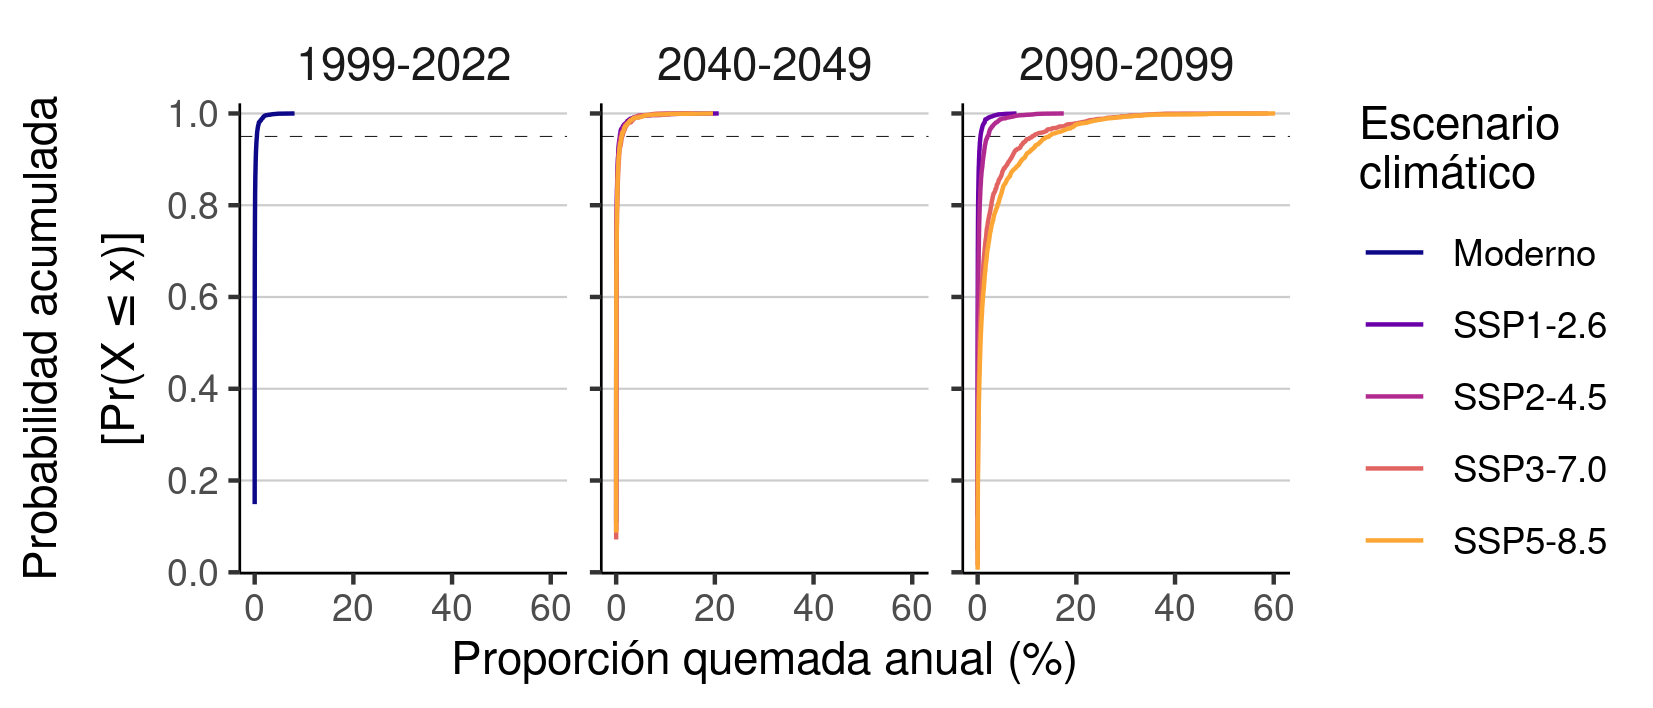
\includegraphics[width=14cm]{figuras/cap4/projections/burn_prob_cdf.png}
  \caption[Distribución de proporción quemada del PNNH bajo escenarios de clima actual y futuro.]{Función de distribución acumulada empírica para la proporción quemada anual del PNNH por experimento. El eje Y indica la probabilidad de que en una simulación la proporción quemada sea menor o igual al valor indicado en el eje X, con la línea discontinua indicando Pr = 0.95. Las curvas se extienden a lo largo del eje X entre el rango observado de proporción quemada. El valor en Y en donde comienzan las curvas indica la proporción de simulaciones sin fuego por experimento.}
  \label{fig:proj-cdf}
\end{figure}


\begin{table}[ht]
\centering
\caption[Proporción quemada del PNNH bajo escenarios de clima actual y futuro.]{Proporción del PNNH quemada anualmente y proporción quemada por rayos sobre el total quemado por experimento. Los factores de cambio son el cociente de la media estimada sobre la media en el período 1999-2022. Los valores representan la media de la distribución posterior, con el intervalo de máxima densidad del 95 \% entre corchetes.}
\label{tab:burn-prob-means}
%\scriptsize % Reduce el tamaño de la fuente
\begin{adjustbox}{max width=\textwidth}
\begin{tabular}{cc|cc|cc}
\toprule
Período & Escenario & \makecell{Proporción quemada\\anual (\%)} & Factor de cambio & \makecell{Fracción quemada\\por rayos (\%)} & Factor de cambio \\
\midrule
1999-2022 & Moderno & 0.1 [0.09; 0.11] & 1 & 25.31 [23.68; 26.96] & 1\\
\addlinespace
\multirow{4}{*}{2040-2049} & SSP1-2.6 & 0.2 [0.18; 0.22] & 2.07 [1.74; 2.35] & 26.68 [25.08; 28.28] & 1.06 [0.96; 1.15]\\
 & SSP2-4.5 & 0.21 [0.19; 0.23] & 2.23 [1.92; 2.55] & 26.06 [24.53; 27.58] & 1.03 [0.94; 1.12]\\
 & SSP3-7.0 & 0.25 [0.23; 0.27] & 2.61 [2.25; 2.98] & 27.41 [25.91; 28.91] & 1.08 [0.99; 1.18]\\
 & SSP5-8.5 & 0.25 [0.22; 0.27] & 2.61 [2.23; 2.98] & 26.84 [25.32; 28.53] & 1.06 [0.97; 1.16]\\
\addlinespace
\multirow{4}{*}{2090-2099} & SSP1-2.6 & 0.13 [0.12; 0.14] & 1.36 [1.17; 1.56] & 26.41 [24.76; 28.06] & 1.04 [0.94; 1.13]\\
 & SSP2-4.5 & 0.42 [0.39; 0.46] & 4.44 [3.87; 5.05] & 27.81 [26.29; 29.37] & 1.1 [1.01; 1.19]\\
 & SSP3-7.0 & 2.33 [2.15; 2.52] & 24.46 [21.44; 27.87] & 33.68 [32.32; 35.13] & 1.33 [1.23; 1.44]\\
 & SSP5-8.5 & 2.97 [2.75; 3.18] & 31.17 [27.53; 35.39] & 34.17 [32.78; 35.53] & 1.35 [1.25; 1.46]\\
\bottomrule
\end{tabular}
\end{adjustbox}
\end{table}

\begin{figure}[htbp]
  \centering 
  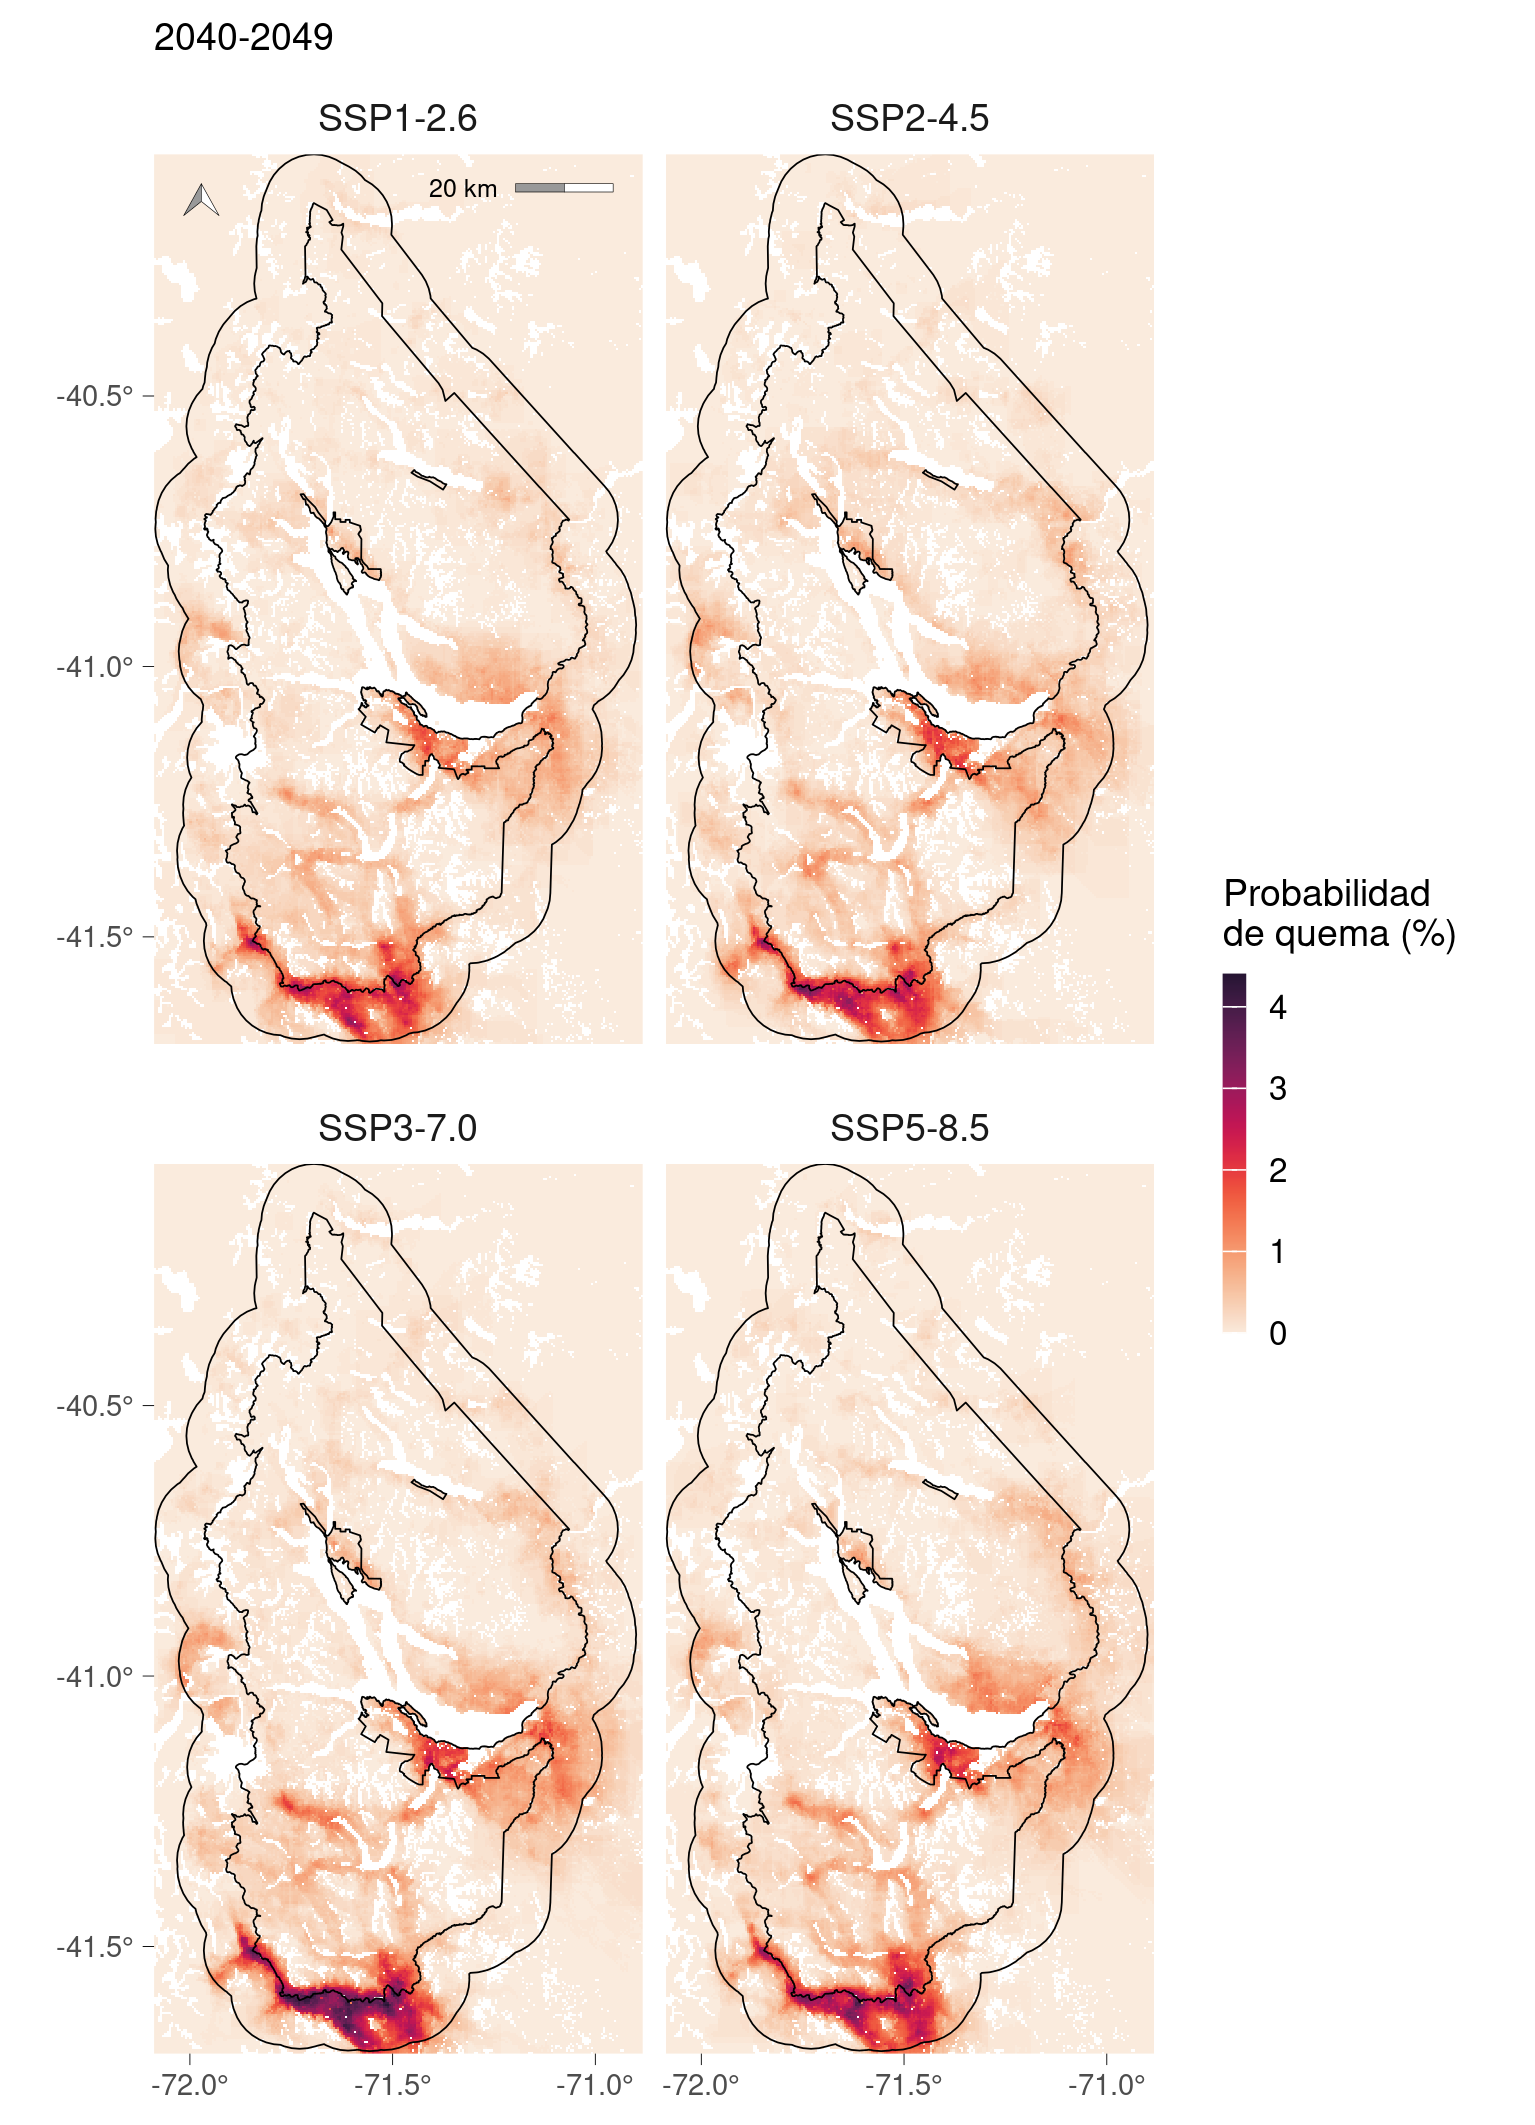
\includegraphics[width=1\textwidth]{figuras/cap4/projections/burn_prob_2040.png}
  \caption[Probabilidad de quema anual en el PNNH proyectada para el período 2040-2049 bajo distintos escenarios climáticos.]{Probabilidad de quema anual en el PNNH proyectada para el período 2040-2049 bajo distintos escenarios climáticos. El contorno exterior indica el área en donde se simularon las igniciones para reducir el efecto borde.}
  \label{fig:proj-2040}
\end{figure}

\begin{figure}[htbp]
  \centering 
  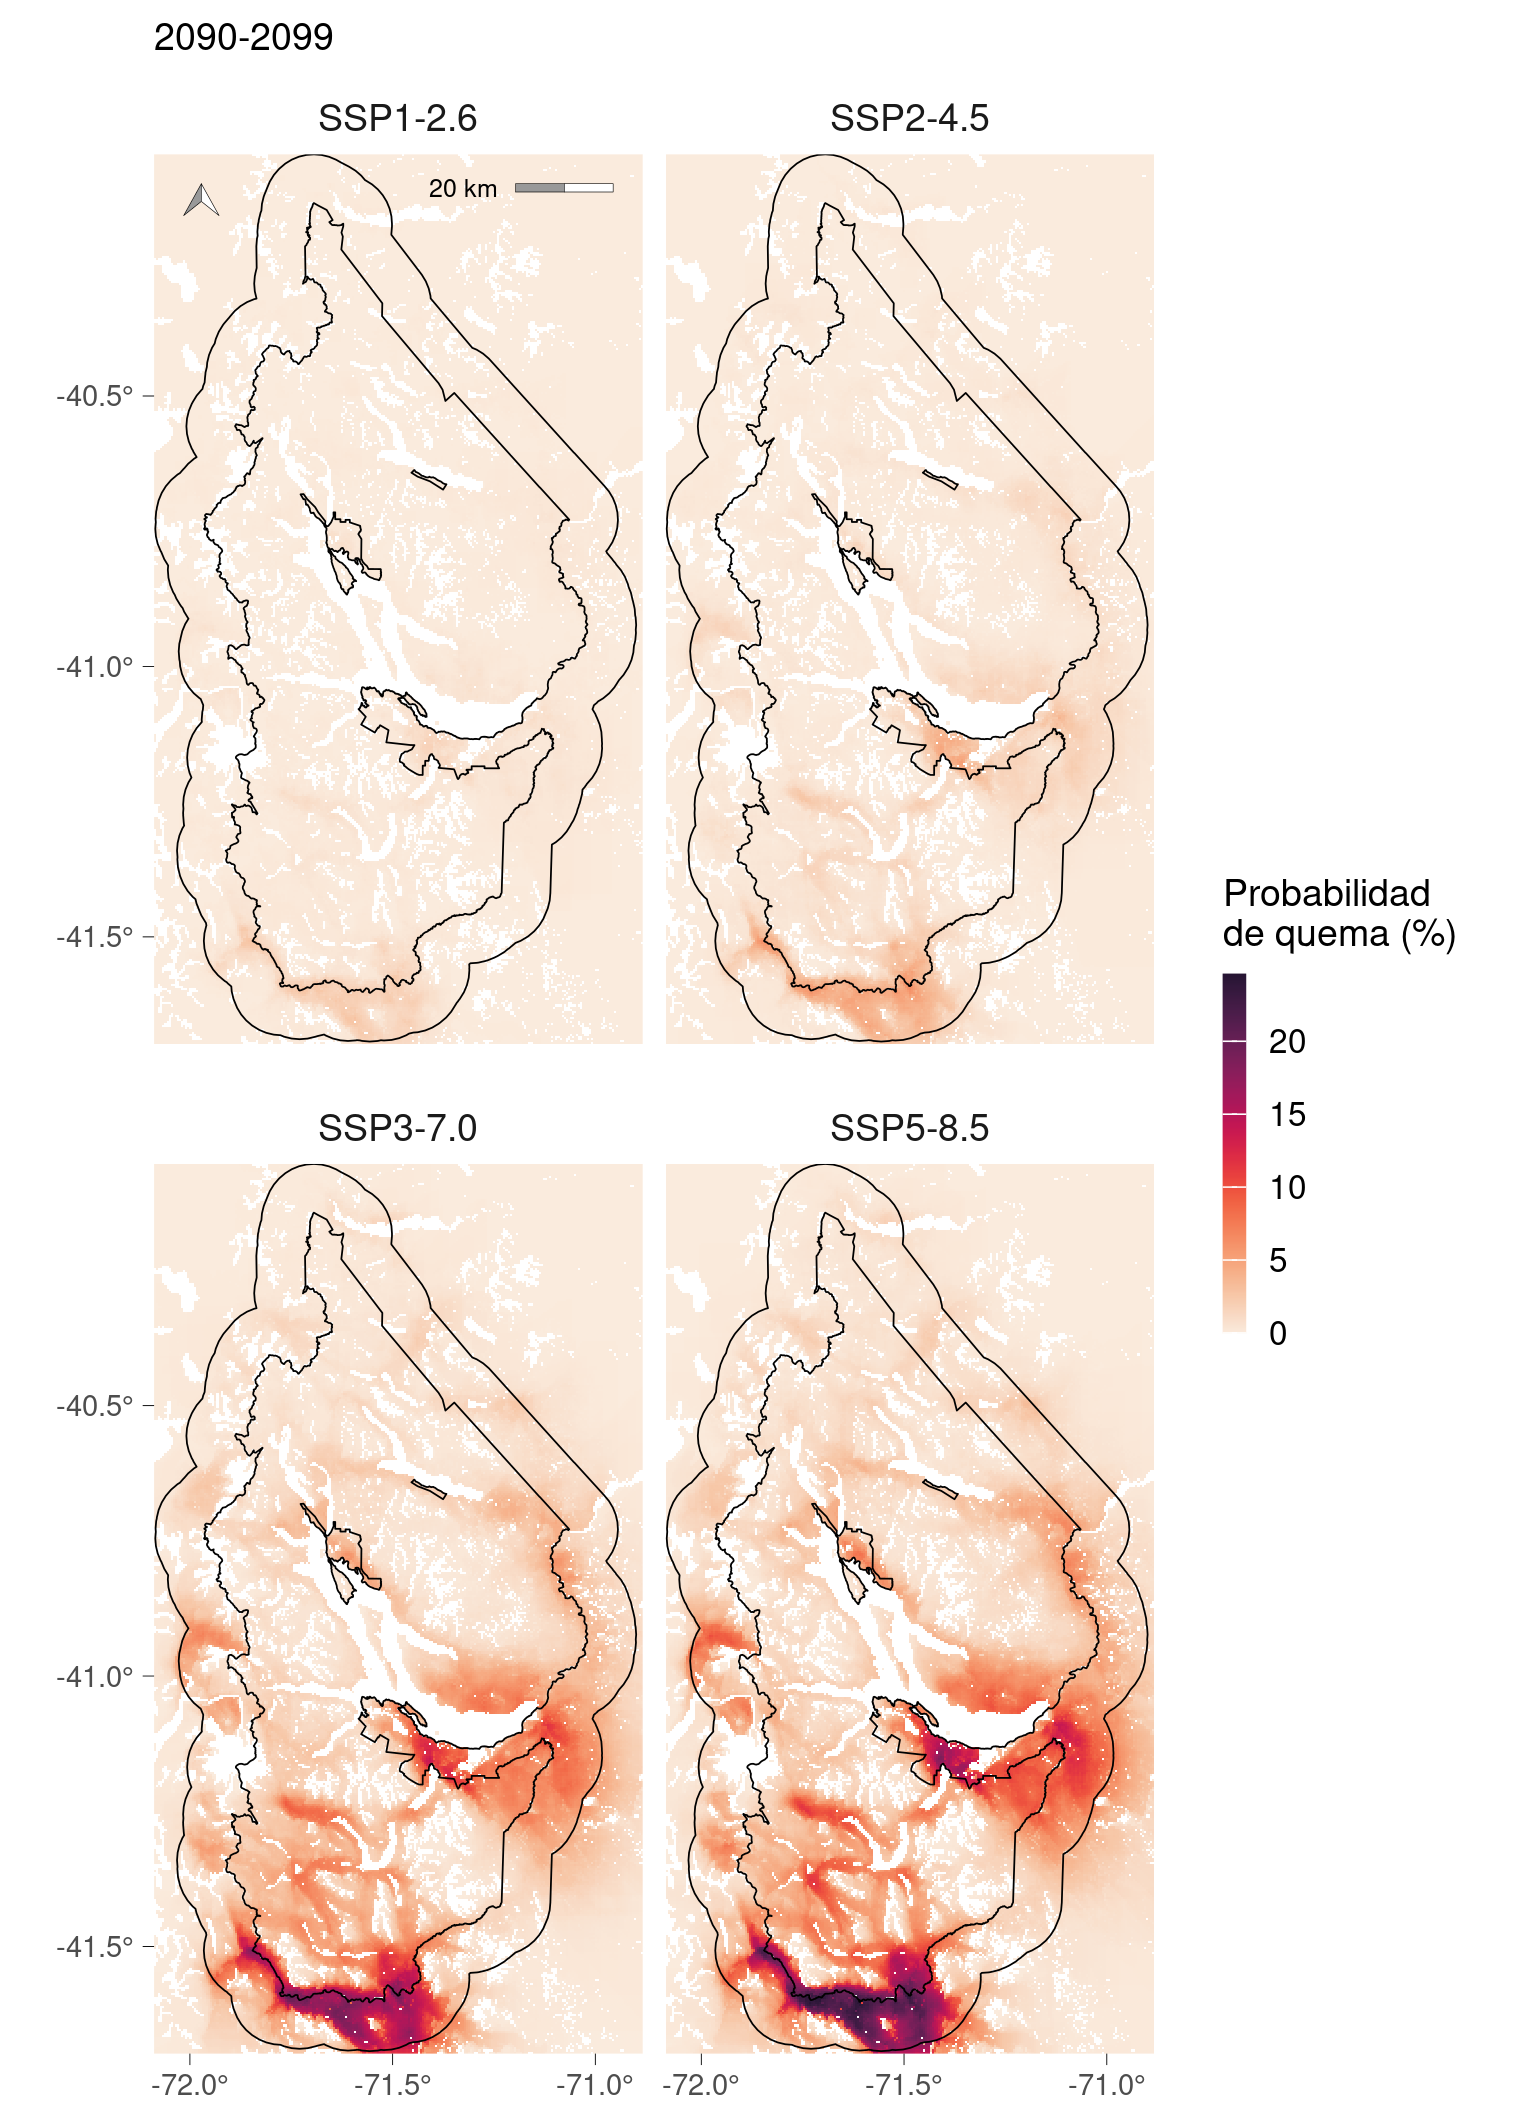
\includegraphics[width=1\textwidth]{figuras/cap4/projections/burn_prob_2090.png}
  \caption[Probabilidad de quema anual en el PNNH proyectada para el período 2090-2099 bajo distintos escenarios climáticos.]{Probabilidad de quema anual en el PNNH proyectada para el período 2090-2099 bajo distintos escenarios climáticos. El contorno exterior indica el área en donde se simularon las igniciones para reducir el efecto borde.}
  \label{fig:proj-2090}
\end{figure}

\FloatBarrier % no projection images below

\section{Discusión}

% overview
En este trabajo desarrollamos modelos de simulación de incendios espacialmente explícitos tomando en cuenta sus principales controles a escala de paisaje, y con ellos estimamos la probabilidad de quema en el PNNH bajo escenarios climáticos futuros. Los resultados sugieren que la incidencia del fuego en esta región se duplicará (2 x) para los 2040s, mientras que para fines de siglo se esperan aumentos menores (1.3 x) o notablemente mayores (31 x), dependiendo del escenario climático.

% discusión modelos puntuales
Los modelos de ignición, escape y propagación reflejaron de forma razonable muchos aspectos conocidos sobre el comportamiento del fuego. Por ejemplo, la tasa de ignición por rayos mostró un aumento más marcado con el FWI que la tasa de ignición por humanos. Esto resulta sensato considerando que, si bien la ocurrencia de focos por ambas causas se relaciona con la meteorología porque dependen de la humedad del combustible, los focos causados por rayos requieren, además, condiciones atmosféricas propicias para la actividad eléctrica \citep{shmuel2024lightning}. En cambio, los focos causados por humanos dependen de la actividad humana, que no necesariamente está tan asociada a condiciones atmosféricas como la ocurrencia de rayos \citep{deDiego2023examining}. A su vez, el aumento en la probabilidad de escape en función de la distancia a caminos y poblados refleja la dificultad para controlar focos remotos \citep{thompson2021forest,kolkos2025evaluation}. 

Quizás los aspectos más llamativos de los modelos desarrollados se encuentren en el modelo de propagación, que al haberse ajustado sin datos de contagio celda a celda, presentaba mayor dificultad para representar la propagación, en comparación con los modelos de ignición y escape. Una de las características más importantes de este modelo es que la probabilidad de propagación depende principalmente de los efectos direccionales del viento y la pendiente, con la vegetación y la topografía (altitud y orientación) tomando roles secundarios \citep{rothermel_mathematical_1972}. Además, la correlación negativa entre los efectos del viento y la pendiente refleja el hecho de que la propagación del fuego tiende a estar dominada por un factor u otro (\citealt{laneri_first_2020}; \cref{fig:spread-corr}). A su vez, el efecto del viento, que representa la velocidad del viento en cada incendio (variable no observada), aumentó con el FWI (Fig.~\ref{fig:spread-params}E); lo cual es coherente con el FWI estando definido como una función creciente de la velocidad del viento, además de la temperatura, humedad del aire, y precipitación. Otro aspecto a destacar fue la correlación positiva entre los pasos de simulación ($\kappa$, ver Ecuación~\ref{eq:datamodel}) y el efecto del viento ($\beta_4$; \cref{fig:spread-corr}): en condiciones de mayor velocidad del viento, los incendios requieren más pasos de simulación, lo que les permite extenderse en la dirección del viento. Esta correlación positiva limita las simulaciones en que el fuego propaga en cualquier dirección durante muchos pasos, lo que generaría incendios extremadamente grandes. 

Si bien el modelo de propagación representó de forma razonable muchos aspectos conocidos sobre la propagación del fuego, su limitada capacidad para simular incendios similares a los ocurridos (utilizando parámetros simulados, Fig.~\ref{fig:spread-ov} y \ref{fig:spread-q}) demuestra que el polígono final y el punto de ignición de los incendios aportan limitada información sobre la propagación. En los últimos años, algunas instituciones encargadas del combate de incendios, como el ICE del PNNH, comenzaron a elaborar polígonos de avance diario de los incendios. A su vez, recientemente se han instalado numerosas estaciones meteorológicas en la región. Con estas nuevas fuentes de datos podremos desarrollar y estimar modelos de propagación más realistas, modelando los efectos del viento y la pendiente sobre la propagación del fuego a mayor resolución temporal y espacial, lo que permitirá cuantificar en forma más detallada el efecto de variables con efectos menos marcados, como la vegetación y la topografía. 

% vegetación

A pesar de la simpleza del modelo de propagación, aportó evidencia relevante desde un punto de vista ecológico: el efecto de la vegetación (IIV) no varió a lo largo de un amplio rango de FWI (Fig.~\ref{fig:spread-curves}A, \ref{fig:spread-params}A y \ref{fig:spread-veg-effects}). Numerosos estudios reportan que los controles locales del fuego (\textit{bottom-up}), como la vegetación y la topografía, tienden a atenuarse bajo condiciones atmosféricas extremas: tipos de combustible o condiciones topográficas que que normalmente limitan la propagación del fuego, pueden dejar de ser una barrera efectiva y permitir una mayor propagación bajo condiciones atmosféricas extremas \citep{Podur2009, Parks2015, Collins2019, jones_extreme_2023}. Sin embargo, encontramos que el efecto de la vegetación, a pesar de ser un control secundario de la probabilidad de propagación, se mantuvo para valores altos de FWI. Esto podría reflejar que, si bien todos los tipos de vegetación pueden arder cuando las condiciones atmosféricas lo permiten, la velocidad de propagación del fuego aún es menor en comunidades boscosas cerradas, debido al mayor contenido de humedad del combustible, su menor continuidad, y la mayor carga de combustibles gruesos que actúan como sumideros de calor \citep{zylstra_biophysical_2016}. Si bien sería esperable que a valores de FWI mayores a los observados en el período de los datos (1998-2022) la probabilidad de propagación tienda a 1 para todos los tipos de vegetación, anulando su efecto, la vegetación aún presenta un control importante para el fuego ante un FWI elevado. Esto resulta relevante a la hora de considerar estrategias de manejo: conservar comunidades boscosas con dosel alto y cerrado podría disminuir la velocidad de propagación del fuego en el paisaje, lo cual disminuiría el área quemada en comparación con paisajes dominados por matorrales \citep{tiribelli_non-additive_2019}. 

% performance

Evaluar el desempeño de modelos de probabilidad de quema (como nuestro simulador del régimen de incendios) es desafiante porque producen salidas a escalas temporales y espaciales amplias (e.g., probabilidad de quema en un área extensa y sobre muchos años), por lo que es dificultoso imposible contar con datos para evaluarlos \citep{parisien2020commentary}. En nuestro caso, utilizamos toda la (escasa) información disponible para ajustarlos, y prácticamente no tenemos información independiente para juzgarlos. A su vez, estos modelos no buscan predecir con precisión eventos puntuales, como dónde se quemará en un año en particular, sino representar posibles características del régimen de incendios ante distintos escenarios. Debido a estas particularidades, este tipo de modelos se evalúa juzgando su solidez conceptual y su utilidad para la toma de decisiones, más que por su capacidad para reproducir incendios observados durante períodos cortos \citep{parisien2020commentary}. Aún así, podemos evaluar si el simulador del régimen de incendios recupera patrones generales observados en los datos.

Siguiendo esta lógica, observamos que la probabilidad de quema anual en el PNNH para el período de los datos (1999-2022) presenta un patrón espacial similar a los resultados del Capítulo~\ref{cap:patrones}, donde la altitud fue uno de los factores más importantes regulando la probabilidad de quema. Sin embargo, algunos aspectos de las simulaciones no parecen tener una buena adecuación a los datos. Por un lado, es probable que la contribución relativa de las igniciones por rayos al área quemada esté subestimada. Para 1999-2022 los modelos estimaron un $\approx$ 25 \% (Fig.~\ref{fig:proj-means}B, Tabla~\ref{tab:burn-prob-means}). Este valor se encuentra dentro del rango registrado para las últimas tres décadas en cuatro parques nacionales de la zona (PNNH, Los Alerces, Lago Puelo y Lanín), con 17 \%, 25 \% y 50 \% en las décadas centradas en 2000, 2010 y 2020, respectivamente (\citeauthor{kitzbergerLightning}, en revisión). Para 1999-2022 pero en el área más extensa estudiada en el Capítulo~\ref{cap:patrones}, no contamos con datos de causa para todos los incendios, pero los dos más grandes, que acumulan casi el 30 \% del área quemada, fueron causados por rayos (San Ramón 1999 y Cholila 2015), sin contar otros de gran extensión también causados por rayos. En el PNNH y en el mismo período no contamos con la causa de algunos de los fuegos más grandes, pero la contribución relativa de rayos sería de al menos 46.83 \%. Sin embargo, este valor fue altamente influido por el fuego más grande registrado en el período (Complejo Steffen-Martin 2022). A su vez, el reciente incendio de Los Manzanos (sur del PNNH, verano de 2025), causado por un rayo, constituye uno de los más grandes registrados en el PNNH, aumentando aún más la contribución relativa de los rayos. Si bien la contribución al área quemada de cada fuente de igniciones (rayos-humanos) requiere muchos años de datos porque depende fuertemente de eventos extremos, los modelos aquí desarrollados parecen subestimar la importancia de los rayos en el área quemada total. Esto probablemente se deba a que los incendios generados por rayos, ocurriendo lejos de caminos y poblados, presentan una alta dificultad para el combate no sólo en su momento inicial, sino en todo su desarrollo \citep{thompson2021forest,kolkos2025evaluation}. Nuestros modelos sólo consideran esta mayor dificultad aumentando su probabilidad de escape. Una forma de mejorar este aspecto sería incluir la distancia a caminos y a poblados como predictoras del número de pasos de simulación ($\kappa$) en el modelo de propagación. A su vez, más allá de nuestra posible subestimación de la contribución de relativa de los rayos al área quemada para el período 1999-2022, los aumentos bajo clima futuro parecen presentar problemas mayores. Las condiciones atmosféricas de verano se están volviendo más favorables para la ocurrencia de tormentas eléctricas y para las igniciones por rayos (\citeauthor{kitzbergerLightning}, en revisión), con lo cual, los aumentos proyectados, en factores de $1.06$ y $1.3$ para mediados y fines de siglo, respectivamente (Table~\ref{tab:burn-prob-means}), resultan poco probables, salvo que esperemos un notable aumento en los recursos invertidos en prevención, detección y combate del fuego.

Otro aspecto en que los modelos discrepan de los datos es en la elevada probabilidad de quema predicha en el valle del Manso Inferior, al sur del PNNH. En el periodo de estudio no registramos incendios en esa zona, lo que puede reflejar particularidades de uso humano que resultan en una tasa de ignición por humanos mucho menor que la esperada a esa altitud. Sin embargo, como mencionamos arriba, 24 años de datos en una región con baja incidencia de fuego es poco para juzgar las predicciones de este tipo de modelos \citep{parisien2020commentary}; la ausencia de incendios en esa zona podría ser simplemente azar. De hecho, en el verano de 2025 el incendio de Los Manzanos, generó un foco secundario que llegó a la zona del Valle del Manso Inferior (incendio El Manso).

% proyecciones 

Nuestras proyecciones de proporción quemada y probabilidad de quema anual se asemejan cualitativamente a los resultados de \citet{kitzberger_projections_2022} para un área más extensa (similar al área de estudio del Capítulo~\ref{cap:patrones}; Fig.~\ref{fig:cap3-01}). En dicho trabajo ajustamos un Random Forest para predecir la probabilidad de quema anual de cada celda en el paisaje en función de variables topográficas, de vegetación, climáticas, indicadores de influencia humana y variables atmosféricas, basado en el producto de área quemada de MODIS \citep{giglio_collection_2018}. Si bien los patrones son similares, en dicho trabajo encontramos mayor variación entre escenarios climáticos para el período 2041-2050. Además, para el período 2091-2100, en \citet{kitzberger_projections_2022} reportamos aumentos notablemente menores, alcanzando un valor de 8 x en algunas partes del paisaje bajo el escenario RCP 8.5 (equivalente a SSP5-8.5), comparado con el aumento máximo de 31 x que encontramos en este trabajo. Aunque parte de la discrepancia puede deberse a diferencias en las bases de datos utilizadas, probablemente se explique principalmente por el modelo utilizado en \citet{kitzberger_projections_2022}. Proyectar probabilidad de quema bajo clima futuro es una tarea de extrapolación, y los Random Forests no son una herramienta adecuada para tal fin, ya que en su formulación clásica sólo pueden predecir valores tan altos como el máximo predicho en el set de datos de entrenamiento (\citealt{zhang2019_RF_enhanced}). Sin habernos percatado de la dificultad de extrapolar, nuestros modelos de simulación inicialmente presentaban el problema opuesto: utilizando funciones exponenciales, el clima futuro quemaba todo el paisaje con facilidad, lo que nos llevó a utilizar funciones sigmoideas (Ecuaciones~\ref{eq:igrate} y \ref{eq:hier1}) para obtener proyecciones razonables. Estos aspectos resaltan los desafíos de realizar proyecciones bajo condiciones climáticas que no fueron previamente observadas \citep{fitzpatrick2018will}. 

Si bien nuestro enfoque de modelado contrasta con el empleado en \citet{kitzberger_projections_2022} porque descompusimos en más subprocesos la ocurrencia del fuego (ignición, escape y propagación), las proyecciones bajo clima futuro de ambos trabajos comparten una limitación: en ambos casos proyectamos el régimen de incendios ignorando la retroalimentación entre fuego y vegetación. En nuestras simulaciones, e implícitamente en las proyecciones de \citet{kitzberger_projections_2022} suponemos que la vegetación se mantiene intacta luego de ser quemada, pudiendo quemarse nuevamente al año siguiente, sin considerar regeneración, sucesión, ni transiciones hacia otros tipos de vegetación. Nuestros modelos de simulación fueron concebidos con el objetivo de ser integrados en un modelo dinámico de vegetación que permita modelar explícitamente esta retroalimentación, pero hasta que dicho modelo sea implementado, debemos evaluar con cautela las proyecciones basadas en una capa de vegetación que se reinicia en cada simulación. En esta región, ignorar los efectos de la vegetación puede tener dos efectos opuestos. Primero, si cada año de simulación utiliza vegetación en su mayoría no quemada y, por lo tanto, quemable, la probabilidad de quema se puede sobrestimar, ya que la vegetación puede tardar entre 2 y 20 años en recuperarse y poder propagar fuego con facilidad \citep{tiribelli_changes_2018, tiribelli_non-additive_2019}. Pero esto sería problemático únicamente en zonas o escenarios climáticos en donde el intervalo de retorno del fuego es corto. Bajo clima actual, la zona con mayor probabilidad de quema anual (Manso Inferior) alcanza el 2 \%, lo que implica un retorno medio de 50 años ($1/0.02$); para 2040-2049, en esa zona se proyecta una probabilidad de quema del 4 \%, implicando un intervalo de retorno de 25 años, y para 2090-2099, el tiempo de retorno sería de 4 años. En casos como los últimos dos, la probabilidad de quema probablemente esté ligeramente sobrestimada, pero no en el resto del paisaje, donde la probabilidad de quema es notablemente menor. El otro efecto de asumir vegetación estática es que se ignoran las transiciones hacia otros tipos de vegetación tras el paso del fuego \citep{kitzberger_firevegetation_2016}. Los bosques tienden a ser reemplazados por matorrales si el fuego no deja semilleros vivos a cortas distancias \citep{landesmann_importance_2018,landesmann_increased_2021}, lo cual es frecuente \citep{tiribelli2024spatial}, y si las precipitaciones son escasas \citep{cuevas_tree_2000,kitzberger_effects_2005,tercero-bucardo_field_2007}, que, a su vez, están disminuyendo con el cambio climático (Tabla~\ref{tab:climate-ts}). De esta manera, es probable que nuestras proyecciones sean conservativas, ya que la transición de bosques a matorrales aumentaría la inflamabilidad del paisaje (\citealt{mermoz_landscape_2005,paritsis_positive_2015,morales_stochastic_2015,tiribelli_changes_2018,tiribelli_non-additive_2019}; Capítulo~\ref{cap:patrones}). A su vez, más allá de las transiciones de bosque a matorral causadas por fuego, el cambio climático podría aumentar la inflamabilidad de los bosques a través de los efectos a mediano y largo plazo de las sequías. La mayor frecuencia y severidad de sequías puede aumentar la mortalidad de los árboles que conforman el dosel y la mortalidad parcial de copa \citep{suarez2004factors,rodriguez2016influence,molowny2017changes}. Esto disminuiría la cobertura del dosel, pudiendo resultar en menor humedad de combustible \citep{barbera_microclimate_2023} y promoviendo el desarrollo de la vegetación del sotobosque, lo que aumentaría la continuidad del combustible. Además, esto aumentaría la cantidad de combustible muerto en pie. Pero estos aspectos deben ser analizados con modelos dinámicos de vegetación, ya que también se debe considerar cómo el aumento en la concentración de $\text{CO}_2$ atmosférico puede aumetar la eficiencia fotosintética de las plantas, haciéndolas más tolerantes a las altas temperaturas y a las sequías \citep{silva2013probing,sperlich2020gains}. Este proceso, podría atenuar la mayor mortalidad de árboles que se espera bajo clima futuro \citep{gutierrez2014increased,sperlich2020gains}.

% implicancias-manejo

Si bien nuestras proyecciones ofrecen un escenario posible bajo ciertas condiciones climáticas y sociales, es importante remarcar que en este trabajo suponemos que la tasa de ignición humana y la eficiencia de la prevención y control del fuego se mantienen como en el período 1999-2022). Esto podría implicar una notable sobreestimación de la incidencia del fuego si, en las próximas décadas, se lograran avances significativos en la reducción de igniciones humanas, en la detección temprana de incendios causados por rayos y en el combate. Sin embargo, también es necesario considerar que nuestras proyecciones no incorporan el probable aumento en la frecuencia de tormentas eléctricas (\citeauthor{kitzbergerLightning}, en revisión), lo que volvería aún más improbable un escenario optimista si no se contrarresta con mejoras sustanciales en el combate del fuego. En este contexto, disminuir las igniciones por humanos debería ser una de las estrategias más convenientes. Sin embargo, las igniciones humanas están asociadas a condiciones socioeconómicas desfavorables (e.g., alta tasa de desempleo) y a una alta densidad poblacional \citep{buhler2013demography}, por lo que se requerirían políticas de largo plazo para reducirlas, no sólo campañas de prevención en la estación seca en formato de propaganda. Un ejemplo cercano que ilustra la dificultad de reducir las igniciones antrópicas son las sierras de Córdoba. En dicha región se quema entre un 1.3 y un 3.2 \% del paisaje anualmente (\citealt{arganaraz_incidencia_2020}; cercano a los peores escenarios climáticos para PNNH en los 2090s), y la gran mayoría de los incendios son causados por humanos.

% (párrafo viejo :)

% Una mayor incidencia de incendios generaría mayor gasto en minimizar los daños a la vida humana y la infraestructura, y probablemente generaría una transformación del bosque andino-patagónico, perdiendo representatividad de comunidades boscosas a favor de una mayor abundancia de matorrales \citep{kitzberger_firevegetation_2016,kitzberger_projections_2022}. Las igniciones por rayos aumentarán con el cambio climático (\citealt{perez2023variation}, \citeauthor{kitzbergerLightning}, en revisión) y no pueden ser evitadas, con lo cual se debería invertir en su rápida detección y en aumentar la efectividad del combate inicial para reducir sus impactos. En comparación, disminuir las igniciones por humanos debería ser más factible. Sin embargo, las igniciones humanas están asociadas a condiciones socioeconómicas desfavorables (e.g., alta tasa de desempleo) y a una alta densidad poblacional \citep{buhler2013demography}, por lo que se requerirían políticas de largo plazo para reducirlas, no sólo campañas de prevención en la estación seca en formato de propaganda. Un ejemplo cercano que ilustra la dificultad de reducir las igniciones antrópicas son las sierras de Córdoba. En dicha región se quema entre un 1.3 y un 3.2 \% del paisaje anualmente (\citealt{arganaraz_incidencia_2020}; cercano a los peores escenarios climáticos para PNNH en los 2090s), y la gran mayoría de los incendios son causados por humanos.

% fin

Este trabajo presenta un avance considerable en los esfuerzos de modelado para predecir y proyectar la incidencia del fuego y los patrones de vegetación en el norte de la Patagonia Andina. En el futuro podremos integrar distintos modelos en una plataforma que permita su continua actualización y validación (e.g., \texttt{SpaDES}; \citealt{barros2023empowering, SpaDES}). Para generar proyecciones confiables, será necesario avanzar en el entendimiento de la relación entre condiciones atmosféricas y la incidencia de rayos, los factores que regulan las igniciones humanas, y las respuestas de la vegetación al cambio climático, tanto mediadas por fuego como por otros factores. 